\section{Objetivo general}
El objetivo general del trabajo de la asignatura es el de fomentar la
comprensión de los conceptos que se abordan a lo largo del curso, en
particular los relativos a la obtención de modelo lineal de una
planta, discretización y efecto del muestreo, análisis de la respuesta
transitoria y permanente continua y discreta, lugar de las raíces en
el plano s y z, efecto del retardo y diseño de controlador analógico y
digital PID en sus diferentes métodos, así como el control en espacio
de estado.

Para ello se parte de un sistema univariable definido por un diagrama
de bloques que representan su dinámica temporal, y se tratará de
obtener su comportamiento dinámico y de diseñar un controlador PID o
en espacio de estado que cumpla unas especificaciones de
funcionamiento.

El trabajo se realizará en formato colaborativo y en grupo de 2 o 3
alumnos bajo un soporte fichero tipo Word, donde se irán detallando
las diferentes tareas secuenciales de las que consta el trabajo
conforme se vayan realizando. Al final se subirá el trabajo en formato
.pdf al Campus Virtual y se realizará una exposición oral del trabajo
por parte del grupo completo al profesor y se evaluará junto con el
contenido del trabajo como calificación de asignatura.

\section{Planteamiento del problema de control}
El objetivo del trabajo es controlar la posición de una carga mecánica
de acuerdo con una posición de consigna, utilizando para ello un
esquema tipo servomecanismo.

El sistema inicialmente está controlado proporcionalmente en base a
una ganancia variable $k_a$ sobre un amplificador electrónico que actúa
en base a la diferencia de posición entre el ángulo de consigna
$\theta r(t)$ y el ángulo de la carga mecánica $\theta L(t)$.

El sistema objeto del control es un motor de CC con tren de engranajes
reductor que tiene acoplado una carga mecánica, cuya función de
transferencia viene indicada en el diagrama de bloques adjunto

con señal de entrada $E_a(s)$ y señal de salida $\theta L(s)$ con
parámetros físicos determinados.

El sistema de control de posición será controlado a través de un
controlador PID analógico que reemplazará al controlador proporcional
con ganancia $k_a$, disponiéndose para ello de un sensor de posición
(potenciómetro) de ganancia $k_R$.

El esquema de control propuesto también permite alternativamente
controlar la velocidad del servomotor, sustituyendo el sensor de
posición por un sensor de velocidad (tacómetro) de ganancia $k_w$.

Por otra parte, se tratará de realizar un control digital PID sobre el
sistema servomotor ya sea en posición o en velocidad, para lo cual se
sustituirá el amplificador por un computador añadiendo los
dispositivos de muestreo y reconstrucción pertinentes.

Finalmente se tratará también la representación en espacio de estado y
el diseño del sistema de control por realimentación del vector de
estado.

\section{Actividades}
\subsection{Actividad 1}
 Ejecutar la aplicación \textsc{parámetros\_servo.m} a través del
\textsc{DNI} del miembro de mayor edad del grupo para calcular los
parámetros del sistema servomotor.

\begin{table}[H]
\centering
\begin{tabular}{|c|c|c|c|c|c|} 
 \hline
  \multicolumn{6}{|c|}{Parámetros} \\
 \hline\hline
$k_i$ & 0.0544 & $b_{eq}$ & 0.0344 & $k_r$ & 3.8197 \\\hline
 $k_b$ & 0.0444 & $R_a$ & 0.3438 & $k_w$ & 1 \\\hline
 $J_{eq}$ & 0.0064 & $L_a$ & 0.0054 & $n$ & 0.1 \\\hline
\end{tabular}
\caption{Tabla de parámetros - DNI de Gonzalo Guilamon Martín}
\label{table:1}
\end{table}
\subsection{Actividad 2}
Obtener la ecuación diferencial del servomotor de posición (en bucle
abierto) a partir de la función de transferencia en $s$.\textbf{Con condiciones iniciales nulas.}
  \vspace{-0.05in}
  \begin{equation}
    \begin{split}
      \dfrac{\theta_L(s)}{E_a(s)} &= \dfrac{nk_i}{s((L_as+R_a)(J_{eq}s+b_{eq})+nk_ik_b)}\\
      nk_iE_a(s) & = \left[s((L_as+R_a)(J_{eq}s+b_{eq})+nk_ik_b)\right]\theta_L(s)\\
      nk_iE_a(s) & = \left[(L_as^2+R_as)(J_{eq}s+b_{eq})+nk_ik_bs\right]\theta_L(s)\\
      nk_iE_a(s) & = \left[J_{eq}L_as^3+b_{eq}L_as^2+R_aJ_{eq}s^2+R_ab_{eq}s+nk_ik_bs\right]\theta_L(s)\\
      nk_iE_a(s) & = s^3\theta_L(s)J_{eq}L_a+s^2\theta_L(s)\left(b_{eq}L_a+(s)R_aJ_{eq}\right)+s\theta_L(s)\left(R_ab_{eq}+nk_ik_b\right)\\
      \mathcal{L}^{-1}\left[ nk_iE_a(s)\right] & = \mathcal{L}^{-1}\left[s^3\theta_L(s)J_{eq}L_a+s^2\theta_L(s)\left(b_{eq}L_a+R_aJ_{eq}\right)+s\theta_L(s)\left(R_ab_{eq}+nk_ik_b\right)\right]\\
       nk_iE_a(t) & = \theta_L'''(t)J_{eq}L_a+\theta_L''(t)\left(b_{eq}L_a+R_aJ_{eq}\right)+\theta_L'(t)\left(R_ab_{eq}+nk_ik_b\right)\\
0 & =
\theta_L'''(t)J_{eq}L_a+\theta_L''(t)\left(b_{eq}L_a+R_aJ_{eq}\right)+\theta_L'(t)\left(R_ab_{eq}+nk_ik_b\right)-nk_iE_a(t)\\
% 0 & = \theta_L'''(t)(0.0064)(0.0054)+\theta_L''(t)\left((0.0344)(0.0054)+(0.0054)(0.0064)\right)+\theta_L'(t)\left((0.3438)(0.0344)+(0.1)(0.0544)(0.0444)\right)-(0.1)(0.0544)E_a(t)\\
0 & = \micro{34.56}\theta_L'''(t)+\micro{220.32}\theta_L''(t)+\mili{12.068}\theta_L'(t)-\mili{5.44}E_a(t)\\
\end{split}
\end{equation}


\subsection{Actividad 3}
Obtener la función de transferencia en $z$ del sistema
servomotor de posición discretizado con $T=0.05$ (en bucle abierto) a
través de \textsc{MATLAB} y obtener la ecuación en diferencias
correspondiente.

Existen otros métodos para discretizar la planta pero solo podemos
usar el \textcolor{blue}{`zoh'} porque da el mejor resultado frente a
la reconstrucción del filtro de primer orden
(\textcolor{blue}{`foh'}).

\begin{tcolorbox}[sharp corners, colframe=bluebox, title= Función de
  transferencia en $z$.]
 $>>>$ Gposicionz = c2d(Gt,T,\textcolor{blue}{`zoh'})
  \vspace*{0.5em}
  \begin{tcolorbox}[sharp corners, colback = white]
    \color{gray}
\begin{verbatim}
Gposicionz =
 
  0.001609 z^2 + 0.003276 z + 0.0003034
  -------------------------------------
  z^3 - 1.801 z^2 + 0.8331 z - 0.03168
 
Sample time: 0.05 seconds
Discrete-time transfer function.
\end{verbatim}
  \end{tcolorbox}%
  \vspace*{0.5em}
\end{tcolorbox}%

Considerando el \textbf{sistema lineal discreto} descrito por la
ecuación en diferencias
\begin{equation}
  y(k+n) + a_1 \cdot y(k+n-1)+...+a_n \cdot y(k) = b_0 \cdot
  u(k+n)+...b_n\cdot u(k)
\end{equation}
con función de transferencia
\begin{equation}
  G(z) = \dfrac{Y(z)}{U(z)} = \dfrac{b_0 \cdot z^n + b_1 \cdot z^{n-1}
  + ... + b_n}{z^n+a_1 \cdot z^{n-1}+ ... + a_n}
\end{equation}
luego podemos usar esto para extraer la función.
\begin{equation}
  G(z) = \dfrac{Y(z)}{U(z)} = \dfrac{0.016 z^2+0.03231z+0.003004}{z^3-1.763z^2+0.7949z-0.03168}
\end{equation}
\begin{equation*}
  n = 3; \ b_1 = 0.0016; \ b_ 2 = 0.03231;\ b_3 = 0.003004;\ a_1 =
  -1.763;\ a_2 = 0.7949; \ a_3 = -0.03168
\end{equation*}
Con los parámetros anteriores podemos calcular la ecuación en
diferencias.
\begin{equation}
  y(k+3)-1.763y(k+2)+0.7949y(k+1)-0.03168y = 0.016u(k+2)+0.03231u(k+1)+0.003004u(k)
\end{equation}
Para confirmar que la conversión continua-discreta ha sido correcta
hemos representado ambas funciones de transferencia en una misma
gráfica, con un entrada impulso.
%\textcolor{red}{DUDA: Calcular la inversa mediante MATLAB o a mano}

\begin{tcolorbox}[sharp corners, colframe=bluebox, title= Funciones de
  transferencia.]
  $>>>$ figure\\
  $>>>$ step(Gposicion)\\
  $>>>$ hold \textcolor{blue}{on}\\
  $>>>$ step(Gposicionz)\\
  $>>>$ xlim([0 1])\\
  $>>>$ title(\textcolor{blue}{`Función de transferencia continua vs discreta.'})\\
  $>>>$ legend(\textcolor{blue}{`Función continua',`Función discreta'})\\
  $>>>$ grid \textcolor{blue}{on}\\
\mkanscode{
\begin{figure}[H]
  \centering
  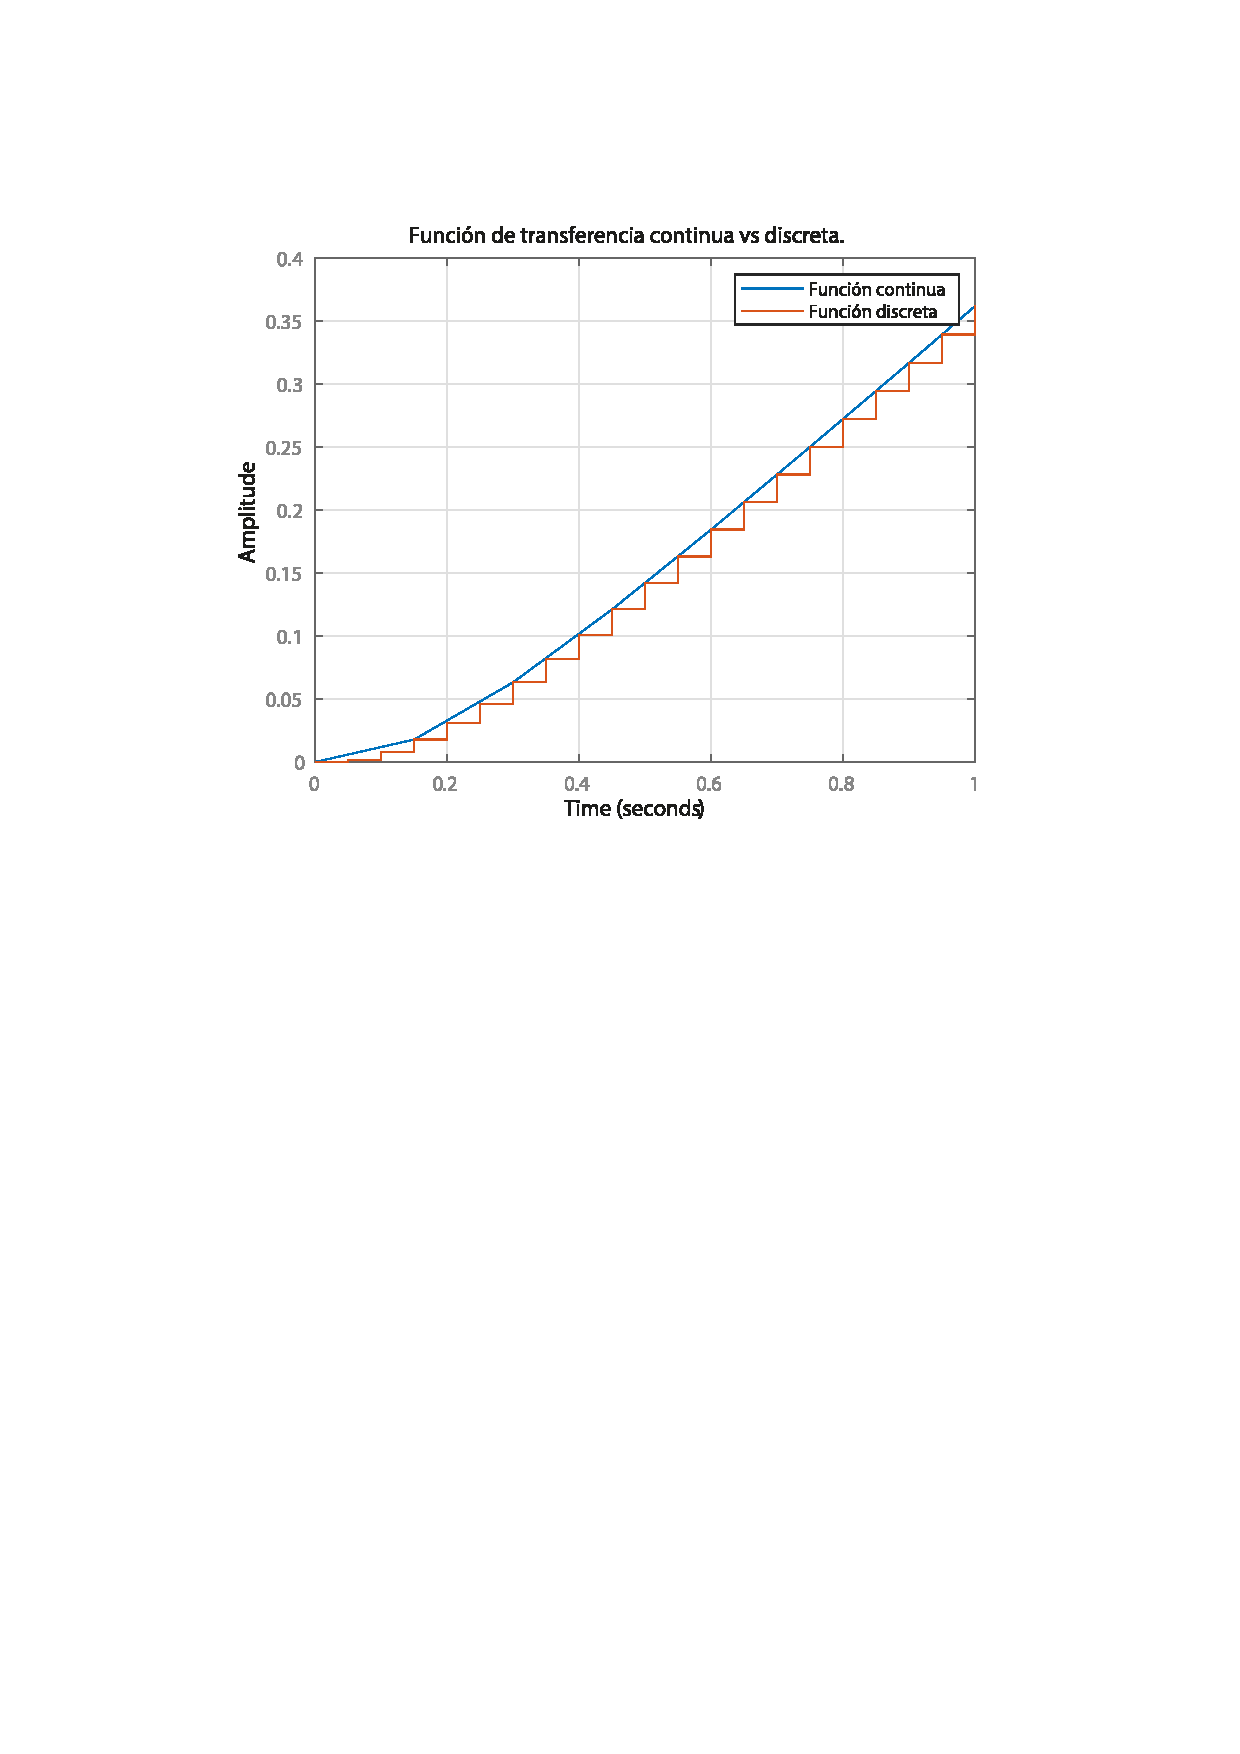
\includegraphics[clip, trim=3.5cm 15.5cm 2cm 3.5cm,
  scale=0.90]{images/figura 1.pdf}
  % izquierda,abajo,derecha,arriba
  \caption{Respuesta de funciones de transferencia frente a una
    rampa.}
    \label{fig:respuesta}
\end{figure}
}
\end{tcolorbox}%


\newpage
\subsection{Actividad 4}
Obtener la descripción en espacio de estado $A$, $B$, $C$ y $D$
del sistema servomotor de velocidad y calcular las matrices $G$, $H$,
$C$ y $D$ del sistema por discretización.

\begin{tcolorbox}[sharp corners, colframe=bluebox, title= Espacio de
  estados continuo.]
$>>>$ [A,B,C,D] = ssdata(ss(Gt))
  \vspace*{0.5em}
  \begin{tcolorbox}[sharp corners, colback = white]
    \color{gray}
\begin{verbatim}
A =
  -69.0417  -21.8248       0
   16.0000         0         0
         0    0.1250         0
B =
     8
     0
     0
C =
         0         0    9.8380
D =
     0
\end{verbatim}
  \end{tcolorbox}%
  \vspace*{0.5em}
\end{tcolorbox}%



\begin{tcolorbox}[sharp corners, colframe=bluebox, title= Espacio de
  estados discretos.]
$>>>$ [G,H,Cz,Dz,T]=ssdata(ss(Gtz))
  \vspace*{0.5em}
  \begin{tcolorbox}[sharp corners, colback = white]
    \color{gray}
\begin{verbatim}
G =
    1.8015   -0.8331    0.1267
    1.0000         0         0
         0    0.2500         0
H =
    0.0625
         0
         0
Cz =
    0.0257    0.0524    0.0194

Dz =
     0
T =
    0.0500
\end{verbatim}
  \end{tcolorbox}%
  \vspace*{0.5em}
\end{tcolorbox}%


\subsection{Actividad 5}
Calcular el error en régimen permanente para el caso de usar
controlador proporcional con ganancia $k_a$, ante entrada escalón y
rampa para los casos continuo y discreto con $T=0.05$ tanto del
sistema servomotor de posición como de velocidad.
\begin{center}
  {\Large\textbf{Posición}}\\
   \textbf{Continuo}
  \end{center}
\begin{equation}
  G(s) = \dfrac{157.41}{s(s+63.55)(s+5.495)} \rightarrow \text{Tipo 1}
\end{equation}
\begin{equation}
    kG(s)H(s) = \dfrac{157.41*kr*k}{s(s+63.55)(s+5.495)} =
  \dfrac{N(s)}{D(s)} 
\end{equation}
Mediante el \textbf{Teorema del valor final} 
\begin{equation}
  e(\infty) = \lim_{t\to\infty}e(t)=\lim_{s\to 0}s\cdot E(s)=
  \lim_{s\to 0}\dfrac{s D(s)}{N(s)+D(s)} \cdot R(s) 
\end{equation}
\begin{itemize}
\item Escalón $R(s) =\dfrac{1}{s}$
  \begin{equation}
    \lim_{s\to 0}\dfrac{s D(s)}{N(s)+D(s)} \cdot \dfrac{kr}{s} =
    \lim_{s\to 0}\dfrac{kr \cdot
      s(s+63.55)(s+5.495)}{601.2590\cdot k+s(s+63.55)(s+5.495)} =
    \dfrac{0}{601.2590\cdot k} = 0
    \end{equation}
  \item Rampa $R(s) = \dfrac{1}{s^2}$
    \begin{equation}
      \small
    \lim_{s\to 0}\dfrac{s D(s)}{N(s)+D(s)} \cdot \dfrac{kr}{s^2} =
    \lim_{s\to 0}\dfrac{kr \cdot
      (s+63.55)(s+5.495)}{601.2590\cdot k+s(s+63.55)(s+5.495)} =
    \dfrac{63.55\cdot5.495\cdot3.8197}{601.2590\cdot k} = \dfrac{2.2185}{k}
    \end{equation}
  \end{itemize}

  \begin{center}
   \textbf{Discreto}
  \end{center}
  Mediante el \textbf{Teorema del valor final}
  \begin{itemize}
\item Escalón $(1-z^{-1})$

  \begin{equation}
    e_{ss}=\lim_{z\to 1} \left[(1-z^{-1})\dfrac{kr}{1+GH(z)}\dfrac{1}{1-z^{-1}}\right]
  \end{equation}
    \begin{equation}
          e_{ss}=\lim_{z\to 1} \left[\dfrac{kr}{1+k_a \dfrac{0.0061465 (z+1.939) (z+0.09724)}{(z-1) (z-0.7598) (z-0.0417)}}\right]
        \end{equation}
            \begin{equation}
          e_{ss}=0
        \end{equation}
        
  \item Rampa $\dfrac{Tz^{-1}}{(1-z^{-1})^2}$
    \begin{equation}
    \lim_{z\to 1} \dfrac{1}{\dfrac{k_a}{zT} \left(\dfrac{0.01609(z+1.939)(z+0.0974)}{(z-0.7598)(z-0.0417)}\right)}
  \end{equation}
    \begin{equation}
e(\infty) = \dfrac{1}{k_a(4.6915)}      
    \end{equation}
  \end{itemize}
  
\begin{center}
  {\Large\textbf{Velocidad}}\\
   \textbf{Continuo}
  \end{center}
\begin{equation}
  G(s) = \dfrac{157.41}{(s+63.55)(s+5.495)} \rightarrow \text{Tipo 0}
\end{equation}
\begin{equation}
    kG(s)H(s) = \dfrac{157.41*k}{(s+63.55)(s+5.495)} =
  \dfrac{N(s)}{D(s)} 
\end{equation}
Mediante el \textbf{Teorema del valor final} 
\begin{equation}
  e(\infty) = \lim_{t\to\infty}e(t)=\lim_{s\to 0}s\cdot E(s)=
  \lim_{s\to 0}\dfrac{s D(s)}{N(s)+D(s)} \cdot R(s) 
\end{equation}
\begin{itemize}
\item Escalón $R(s) =\dfrac{1}{s}$
  \begin{equation}
    \small
    \lim_{s\to 0}\dfrac{s D(s)}{N(s)+D(s)} \cdot \dfrac{kr}{s} =
    \lim_{s\to 0}\dfrac{(s+63.55)(s+5.495)}{157.4 k+(s+63.55)(s+5.495)} =
    \dfrac{349.2072}{157.4k+349.2072} = \dfrac{0.2218}{k+0.2218}
    \end{equation}
  \item Rampa $R(s) = \dfrac{1}{s^2}$
    \begin{equation}
      \small
    \lim_{s\to 0}\dfrac{s D(s)}{N(s)+D(s)} \cdot \dfrac{kr}{s^2} =
    \lim_{s\to 0}\dfrac{(s+63.55)(s+5.495)}{157.4 k+(s+63.55)(s+5.495)}\cdot\dfrac{1}{s} =
 \lim_{s\to 0}\dfrac{(s+63.55)(s+5.495)}{157.4 k+(s+63.55)(s+5.495)}\cdot \lim_{s\to 0}\dfrac{1}{s} = \infty
    \end{equation}
  \end{itemize}

  \begin{center}
   \textbf{Discreto}
  \end{center}
  Mediante el \textbf{Teorema del valor final}
  \begin{itemize}
\item Escalón $(1-z^{-1})$
  \begin{equation}
    e_{ss}=\lim_{z\to 1} \left[(1-z^{-1})\dfrac{kr}{1+GH(z)}\dfrac{1}{1-z^{-1}}\right]
  \end{equation}
    \begin{equation}
          e_{ss}=\lim_{z\to 1} \left[\dfrac{kr}{1+k_a \dfrac{0.077655 (z+0.3364)}{(z-0.7598)(z-0.0417)}}\right]
        \end{equation}
            \begin{equation}
          e_{ss}=\dfrac{1}{1+k_a (0.4508)}
    \end{equation}
  \item Rampa $\dfrac{Tz^{-1}}{(1-z^{-1})^2}$
      \begin{equation}
    e_{ss}=\lim_{z\to 1} \left[(1-z^{-1})\dfrac{kr}{1+GH(z)}\dfrac{Tz^{-1}}{(1-z^{-1})^2}\right]
  \end{equation}
    \begin{equation}
          e_{ss}=\lim_{z\to 1} \left[\dfrac{T\cdot kr}{(1-z^{-1})\cdot
            kr \cdot \dfrac{0.077655(z+0.336)}{(z-0.7598)(z-0.0417)}}\right]
        \end{equation}
            \begin{equation}
          e_{ss}=\infty
    \end{equation}

  \end{itemize}

\newpage
\subsection{Actividad 6}
Aplicar \textsc{ltiview} al sistema servomotor de posición en
bucle cerrado discretizado con ganancia $k_a=1$ y calcular las
especificaciones de respuesta transitoria (t\_subida, t\_pico,
t\_establecimiento, sobreoscilación) ante entrada escalón unitario.
\begin{tcolorbox}[sharp corners, colframe=bluebox, title= Sistema
  servomotor de posición.,breakable=unlimited]
  $>>>$ transient\_ans = kr*feedback(Gposicionz,kr)\\
  $>>>$ ltiview(\textcolor{blue}{`step'},transient\_ans)
  \vspace*{0.35em}
  \begin{tcolorbox}[sharp corners, colback = white]
    \color{gray}
\begin{verbatim}
transient_ans =
 
  0.006147 z^2 + 0.01251 z + 0.001159
  ------------------------------------
  z^3 - 1.795 z^2 + 0.8456 z - 0.03052
 
Sample time: 0.05 seconds
Discrete-time transfer function.
\end{verbatim}
  \end{tcolorbox}%
  \vspace*{0.5em}
  \mkanscode{
\begin{figure}[H]
  \centering
  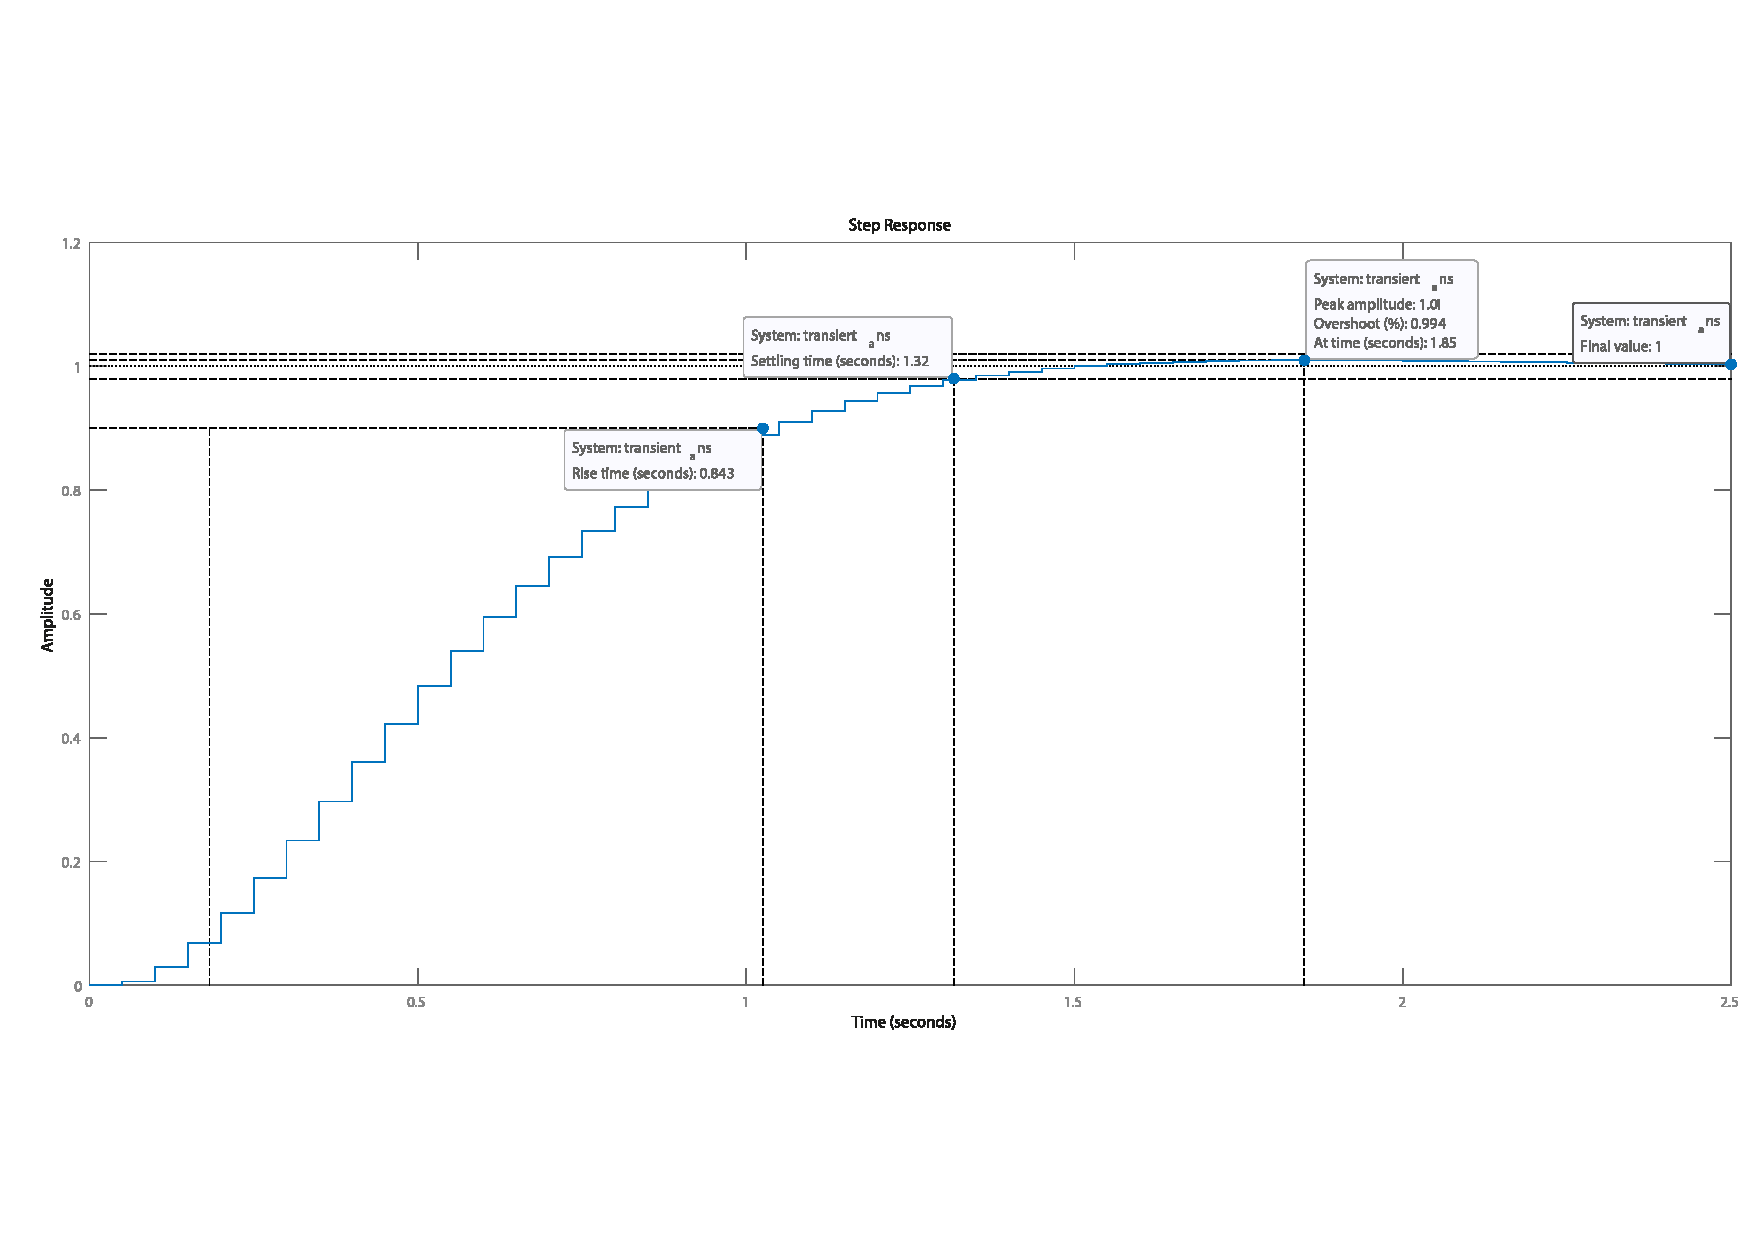
\includegraphics[clip, trim=0.5cm 3.5cm 0.35cm 3.7cm,
  scale=0.48]{images/figura 2.pdf}
  % izquierda,abajo,derecha,arriba
  \caption{Especificaciones de respuesta transitoria en bucle cerrado.}
    \label{fig:comparacion}
\end{figure}
}
\end{tcolorbox}%

\newpage
\subsection{Actividad 7}
Trazar el lugar de las raices discreto en $z$ del sistema
servomotor de posición con \textsc{rltool} y situar los polos en bucle
cerrado para $k_a=1$, $k_a=10$ y calcular los valores de la ganancia
critica para el caso de que el controlador PID discreto sea una
ganancia $k_a$, comentando los resultados.

\begin{tcolorbox}[sharp corners, colframe=bluebox, title= Polos en
  bucle cerrado.,breakable = unlimited]
  $>>>$ rltool(Gposicionz)\\
  \vspace*{0.35em}
  \mkanscode{
\begin{figure}[H]
  \centering
  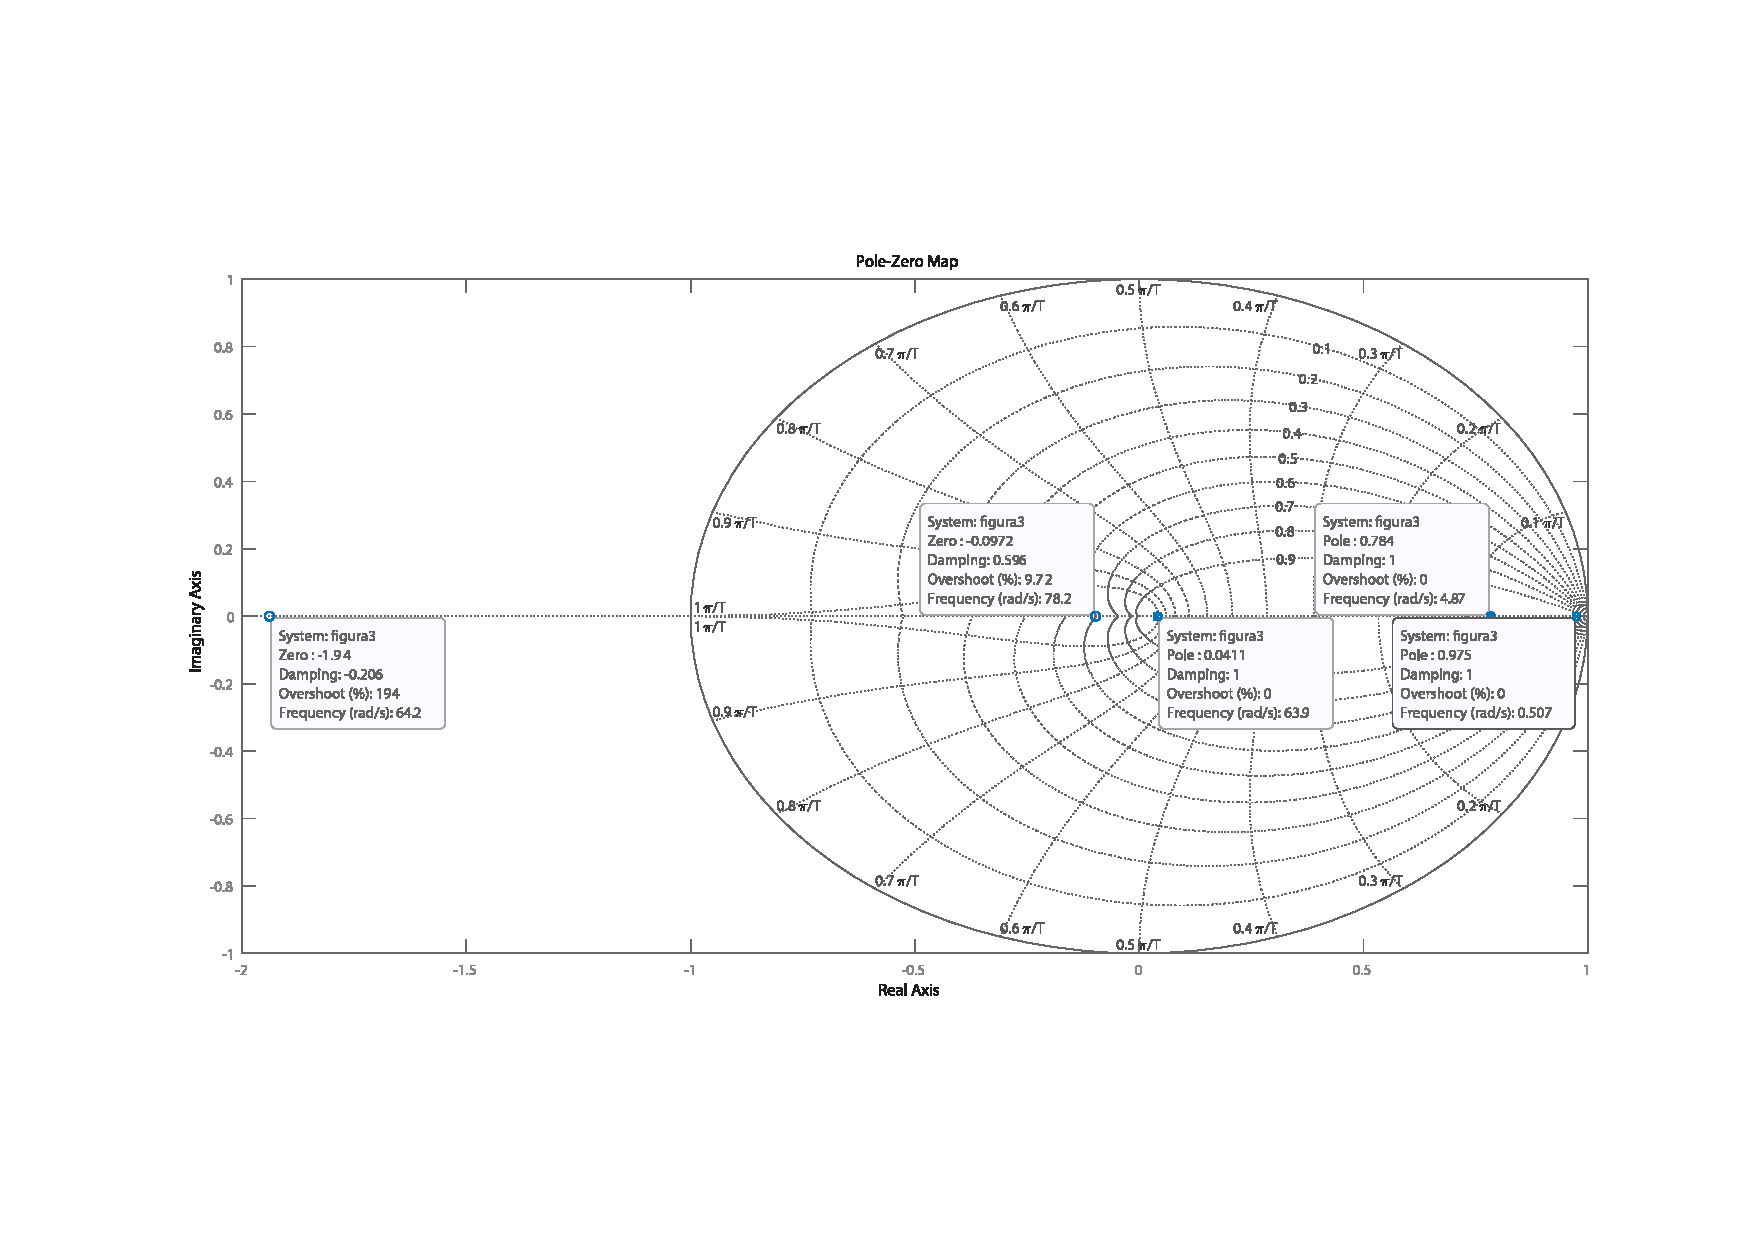
\includegraphics[clip, trim=3cm 4cm 2.8cm 4cm,
  scale=0.48]{images/figura 3.pdf}
  % izquierda,abajo,derecha,arriba
  \caption{Polos en bucle cerrado $k_a = 1$.}
    \label{fig:figura 3}
\end{figure}
}
  \mkanscode{
\begin{figure}[H]
  \centering
  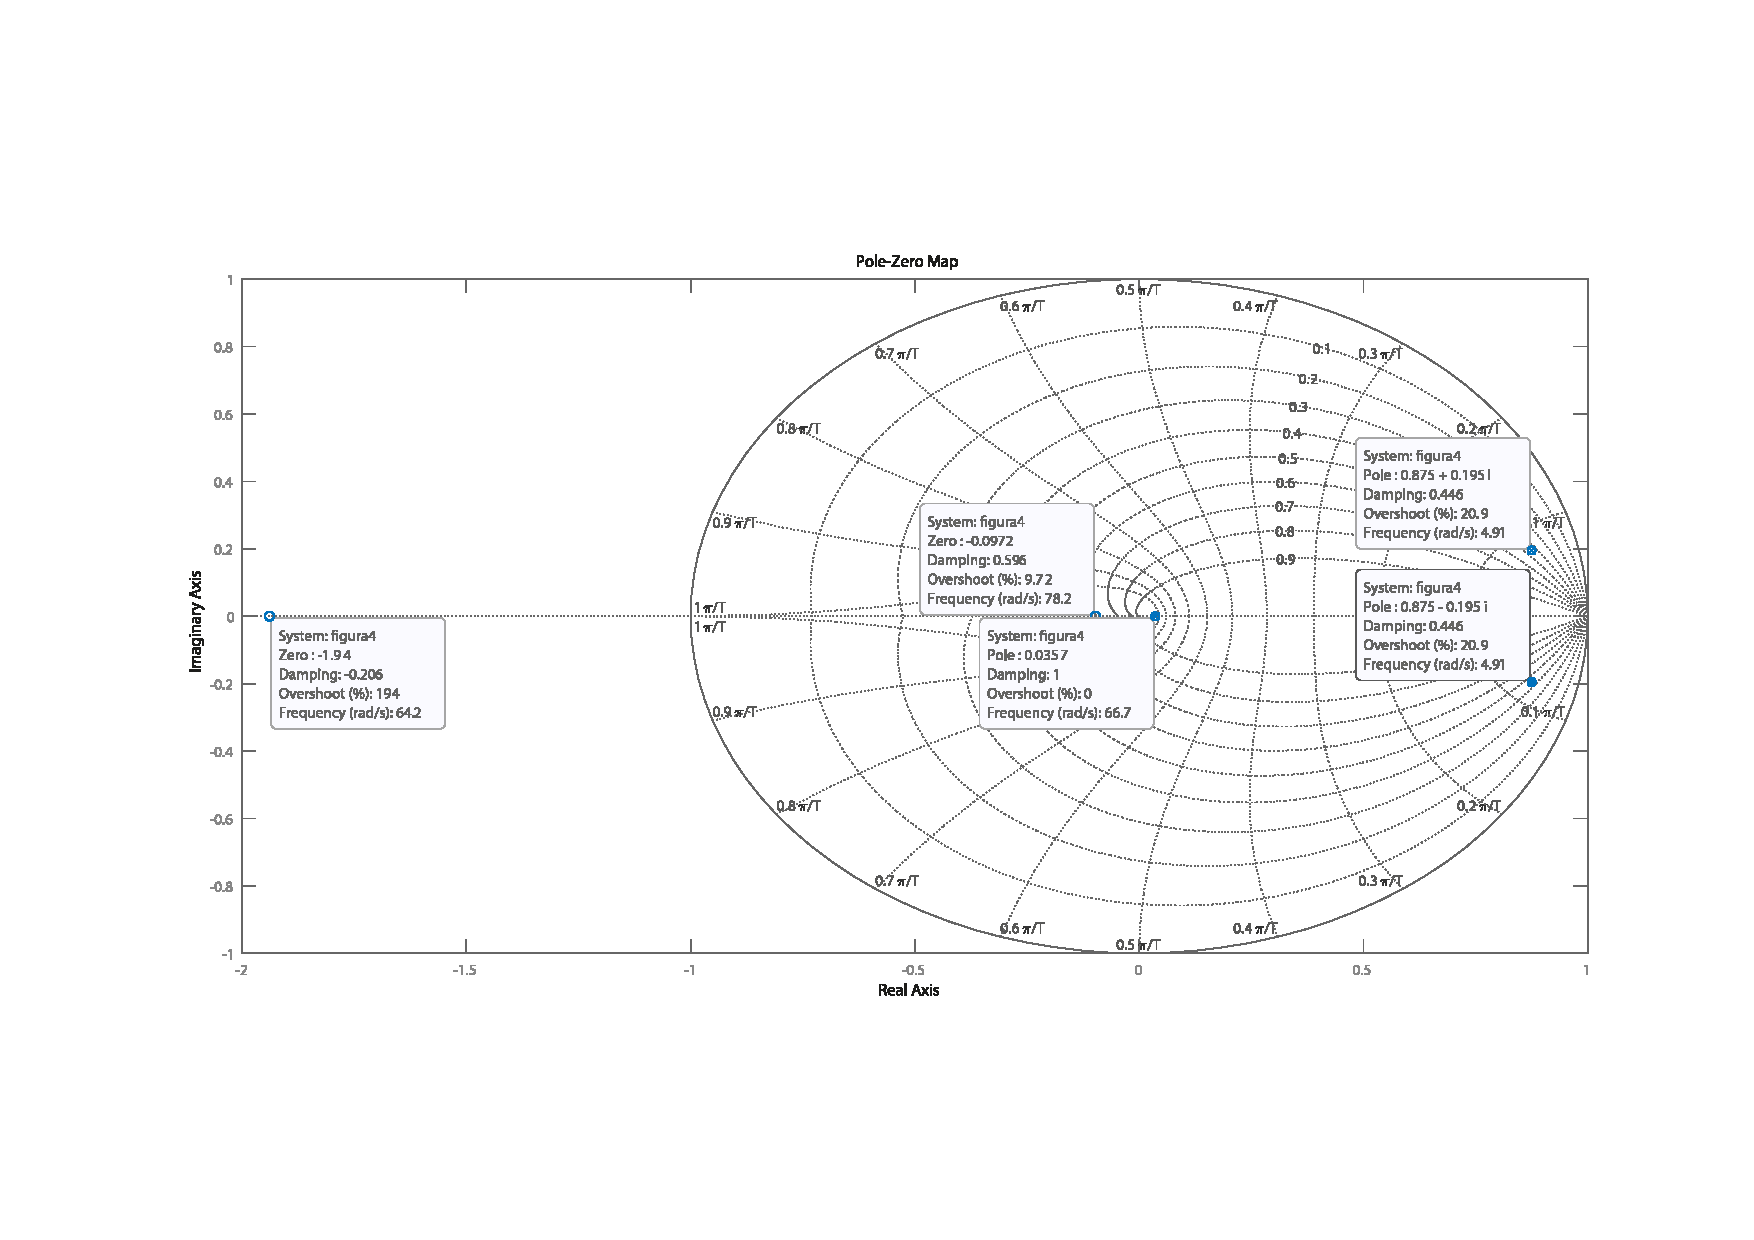
\includegraphics[clip, trim=3cm 4cm 2.8cm 4cm,
  scale=0.48]{images/figura 4.pdf}
  % izquierda,abajo,derecha,arriba
  \caption{Polos en bucle cerrado $k_a = 10$.}
    \label{fig:figura 4}
\end{figure}
}

\end{tcolorbox}%

Mediante rltool y la opción \textsc{New plot > New pole - zero map} podemos
generar una gráfica con los polos según la ganancia que colequemos en
el compensador. Los resultados son los siguientes:

\begin{itemize}
\item $k_a = 1$
  Como se puede observar en la figura \ref{fig:figura 3} los polos son:
  \begin{center}
    \begin{tabular}{ |c|c|c| } 
      \hline
      \multicolumn{3}{|c|}{Polos}\\
      \hline
      0.0393 & 0.878+0.0758$i$ & 0.878-0.0758$i$\\
      \hline
    \end{tabular}
  \end{center}
\item $k_a = 10$
  Como se puede observar en la figura \ref{fig:figura 4} los polos son:
  \begin{center}
    \begin{tabular}{ |c|c|c| } 
      \hline
      \multicolumn{3}{|c|}{Polos}\\
      \hline
      0.0218 & 0.859+0.428$i$ & 0.859-0.428$i$\\
      \hline
    \end{tabular}
\end{center}
\end{itemize}


Para el calculo de la ganancia crítica a través de la herramienta
rltool, variamos la ganancia proporcional hasta llegar al límite de la
estabilidad. 
\begin{center}
$k_{a_{\text{ganancia crítica}}}$  = 15.232
\end{center}

% Otra forma más rápida, usando el comando margin en matlab consguimos
% directamente la gananica crítica, a veces no es exacta pero podemos
% usarla como referencia.


\begin{tcolorbox}[sharp corners, colframe=bluebox, title= Ganancia crítica.]
%   $>>>$ k = margin(Gposicionz)\\
%   \vspace*{0.35em}
%   \begin{tcolorbox}[sharp corners, colback = white]
%     \color{gray}
% \begin{verbatim}
% k =
%    58.1828
% \end{verbatim}
%   \end{tcolorbox}%
    \mkanscode{
\begin{figure}[H]
  \centering
  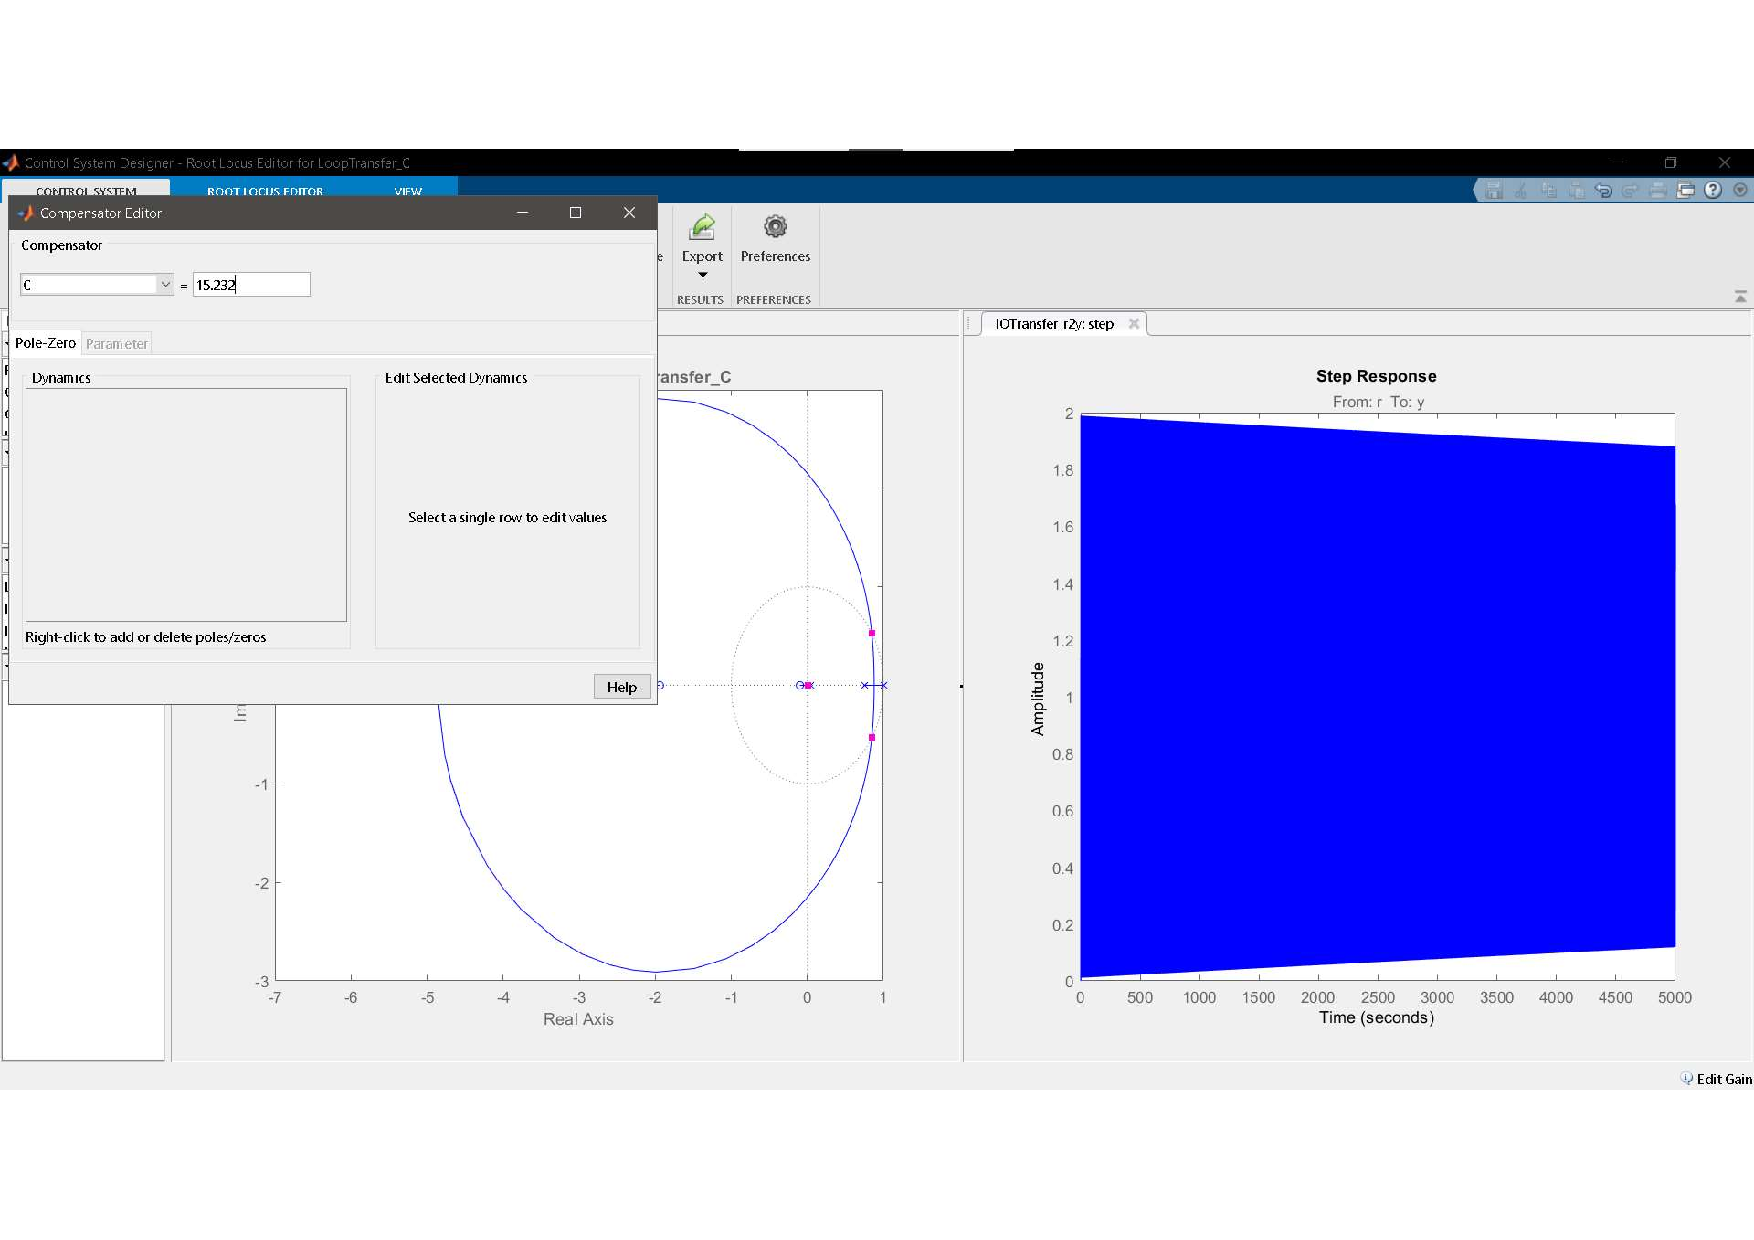
\includegraphics[clip, trim=0cm 2.5cm 0cm 2.5cm,scale=0.48]{images/figura_extra1.pdf}
  % izquierda,abajo,derecha,arriba
  \caption{Rltool - Ganancia crítica.}
    \label{fig:figura extra1}
\end{figure}
  }
\end{tcolorbox}%

\subsection{Actividad 8}
Verificar si es posible compensar en discreto el sistema
servomotor de posición con un controlador proporcional para que el
sistema en bucle cerrado cumpla las especificaciones de
sobreoscilación $< 5 \%$ y tiempo de establecimiento $t_{\text{est}} < 0.3 s$. y
error nulo ante consigna escalón unitaria, graficando la respuesta
escalón.

\begin{tcolorbox}[sharp corners, colframe=bluebox, title= Compensador
  proporcional en tiempo discreto.]
  $>>>$ rltool(Gposicionz)\\
  \vspace*{0.35em}
  \mkanscode{
\begin{figure}[H]
  \centering
  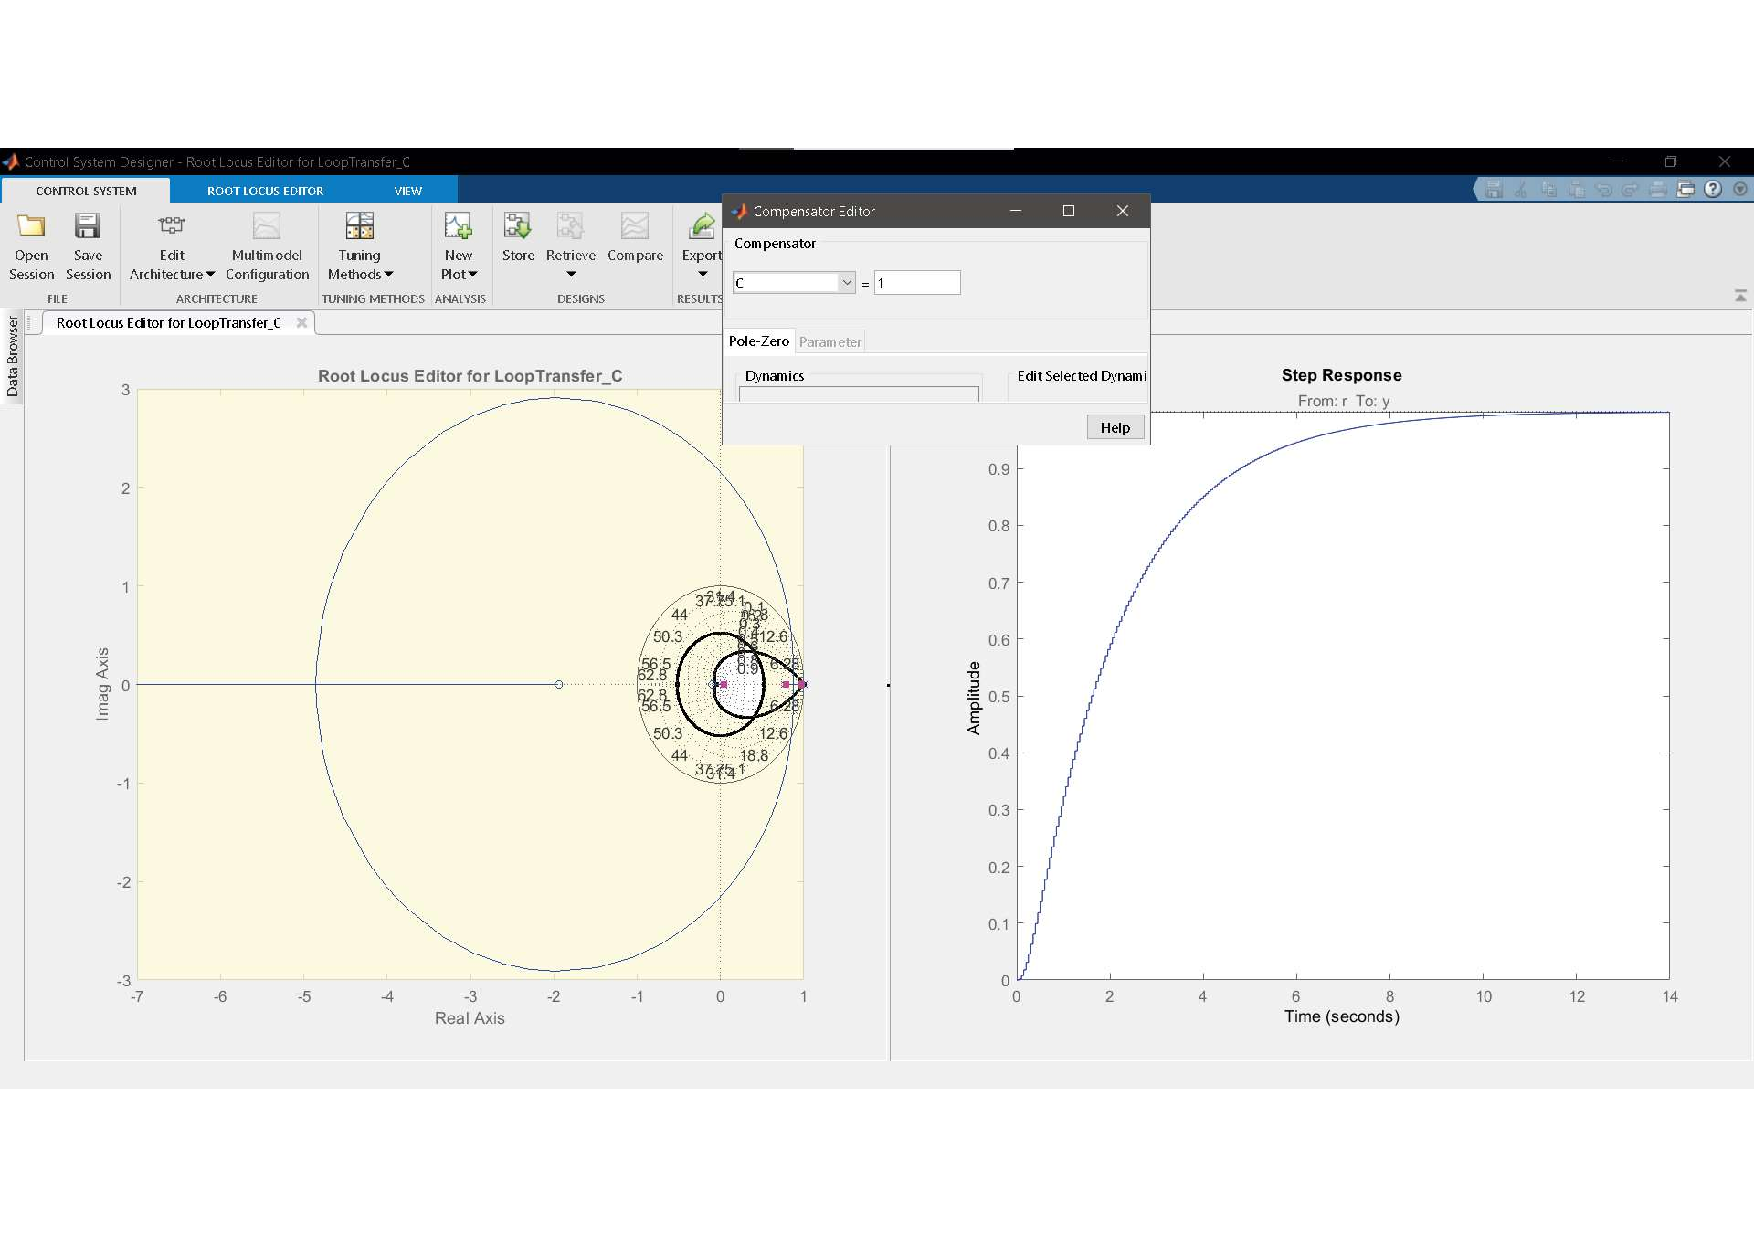
\includegraphics[clip, trim=0cm 3.5cm 0cm 2.4cm,scale=0.45]{images/figura 5.pdf}
  % izquierda,abajo,derecha,arriba
  \caption{Compensador proporcional con ganancia igual a 1.}
    \label{fig:figura 5}
\end{figure}
}

\end{tcolorbox}%

Utilizando el comando \textsc{rltool} con nuestra planta, en la
ventana \textsc{root locus editor} añadimos las especificaciones
necesarias, se puede observar como los polos en bucle cerrado en
nuestro lugar de la raices nunca llegan a cumplir todas las
especificaciones con un control proporcional ya que los polos en bucle
cerrado nunca llegan a la zona blanca sin importar la ganancia
positiva que pongamos.

\newpage
\subsection{Actividad 9}
En caso contrario diseñar un controlador tipo PID digital
implementable (PD, PI o PID) en el lugar de las raíces en $z$ y ver si
es posible cumplir las especificaciones requeridas, expresando el
controlador obtenido, graficando el nuevo lugar de las raíces en $z$,
y comprobando a través de \textsc{ltiview} que se cumplen ciertamente
las especificaciones requeridas.

\begin{tcolorbox}[sharp corners, colframe=bluebox, title= Controlador
  PD con sobreoscilamiento $< 5\%$ y $t_{est} < 0.3$.]
  $>>>$ rltool(Gposicionz)\\
  \vspace*{0.35em}
  \mkanscode{
\begin{figure}[H]
  \centering
  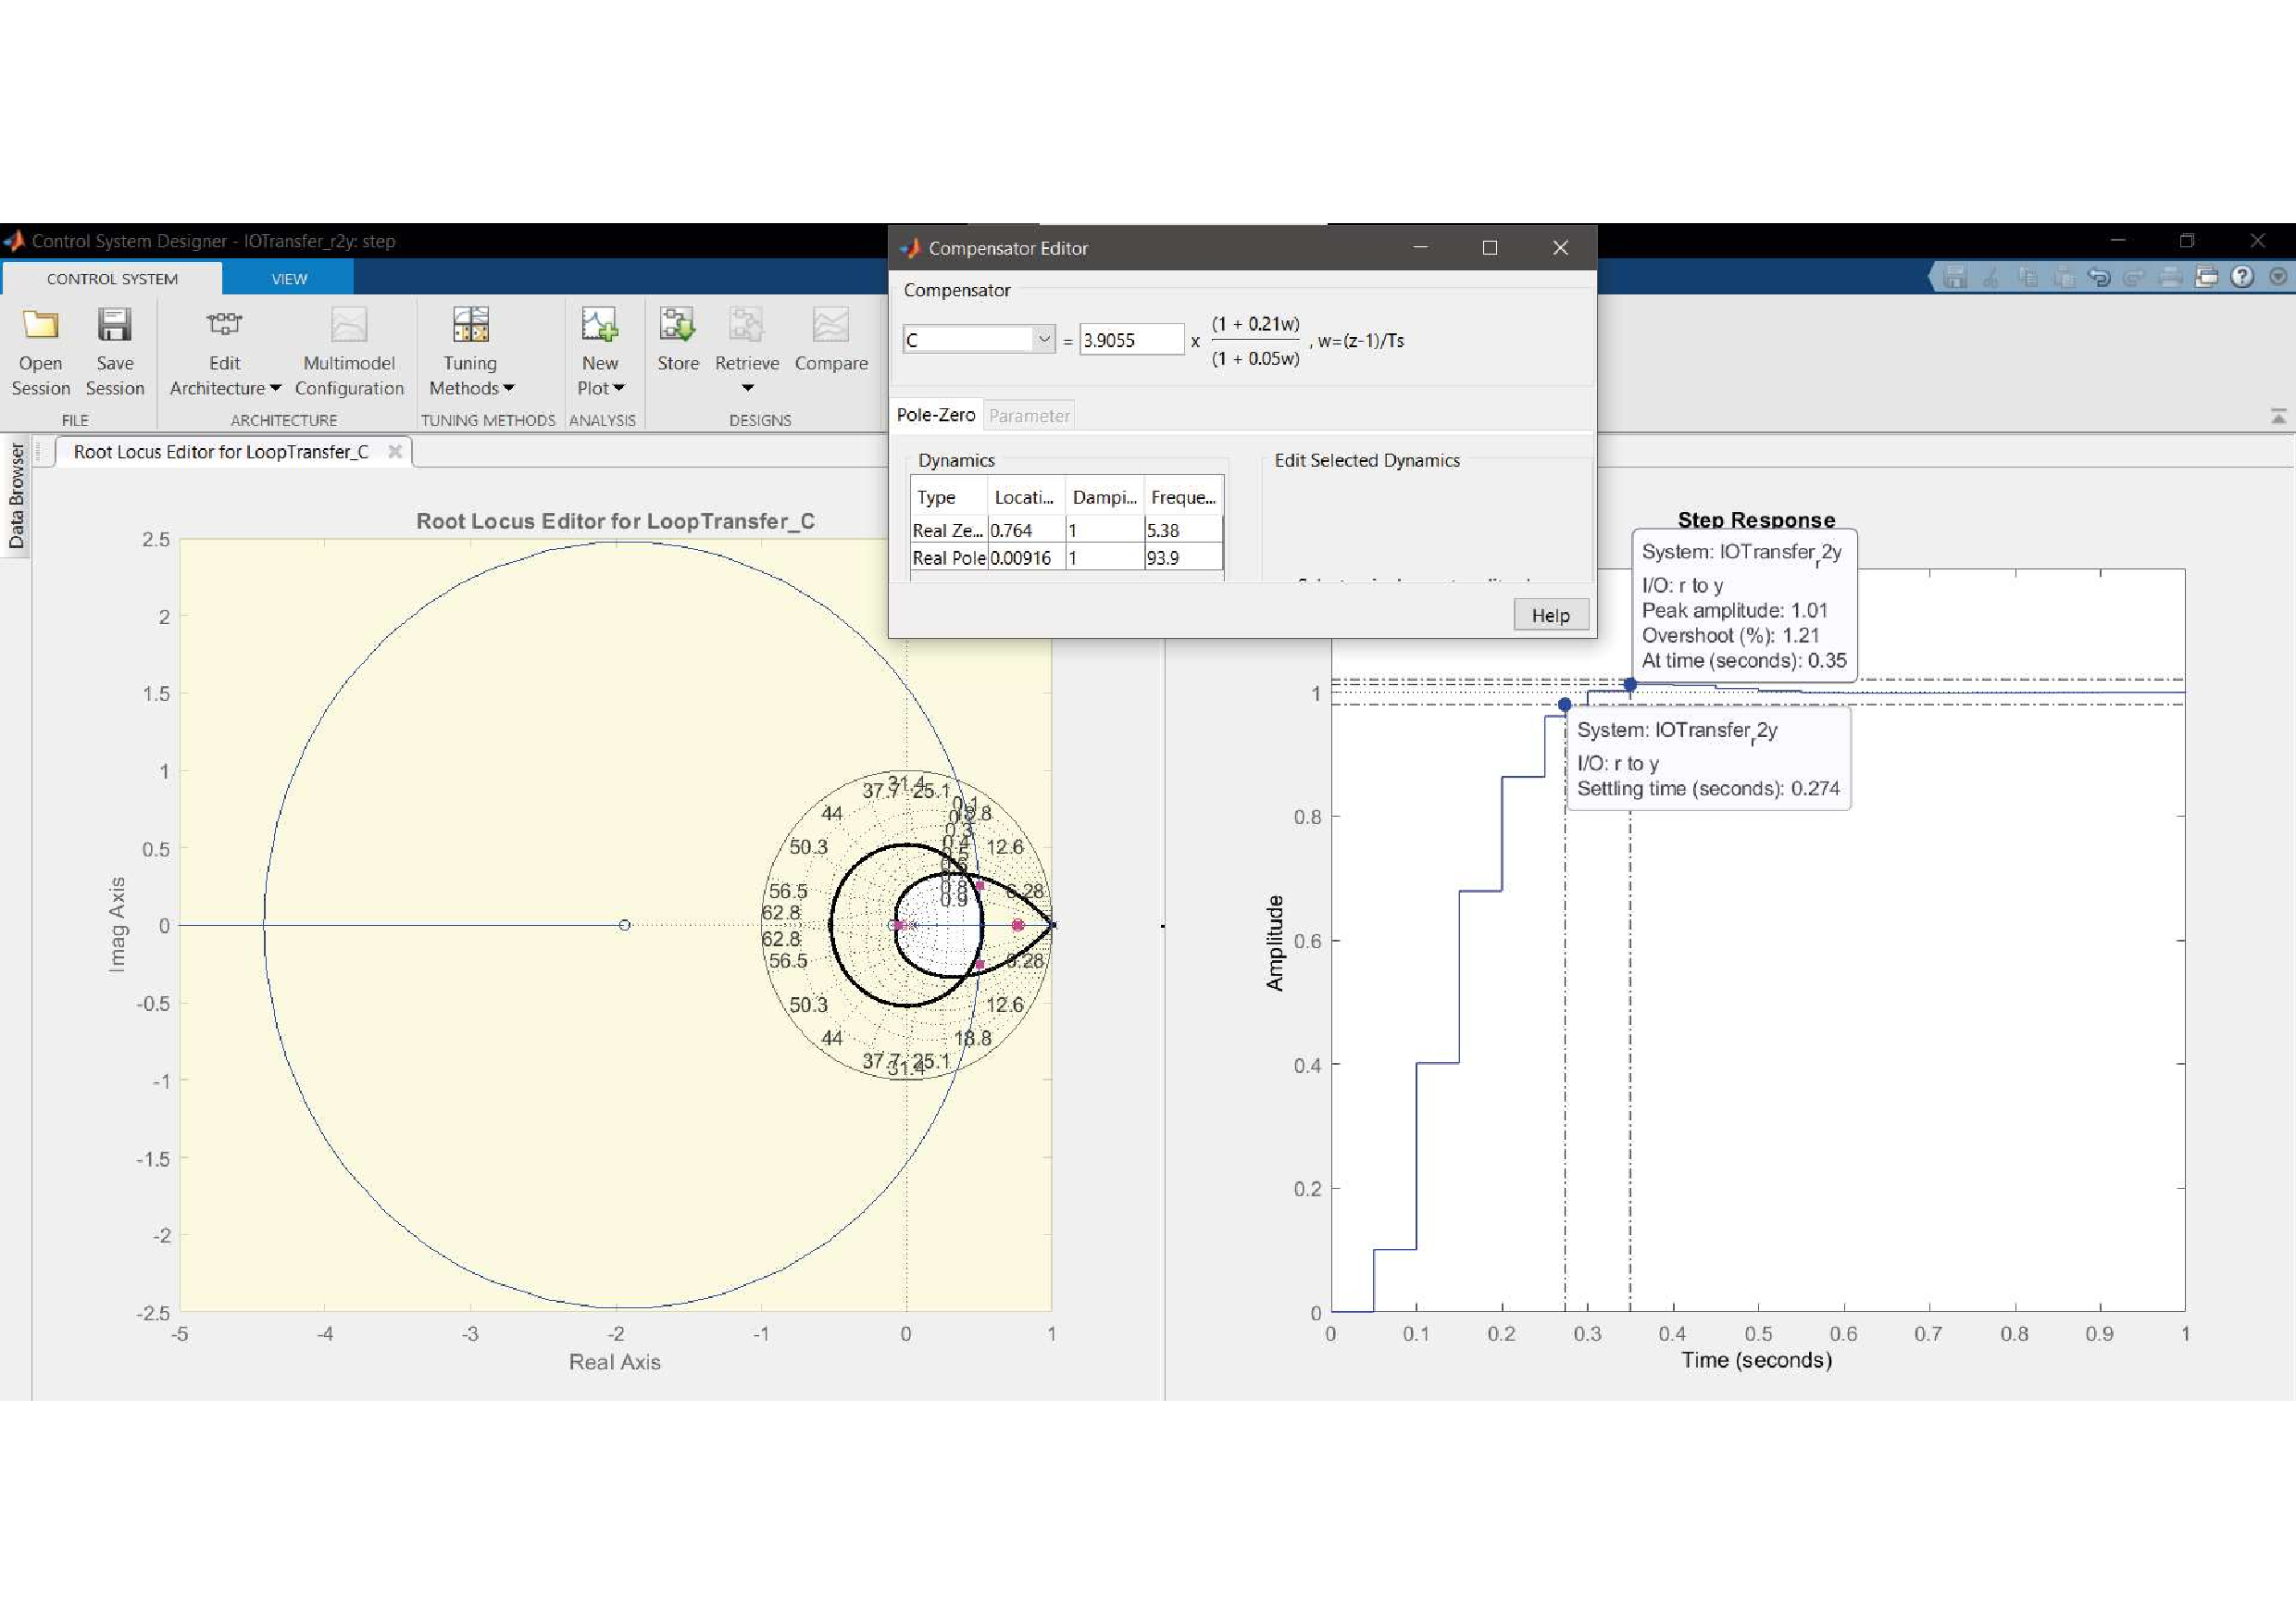
\includegraphics[clip, trim=0cm 4.5cm 0cm 4.2cm,
  scale=0.33]{images/figura 6.pdf}
  % izquierda,abajo,derecha,arriba
  \caption{Controlador PD.}
    \label{fig:figura 6}
\end{figure}
}
\vspace*{0.35em}
Mediante la herramienta \textsc{Export>Export tuned blocks.} podemos
enviar el controlador al espacio de trabajo.

$>>>$ PD\_9
\vspace*{0.35em}
\begin{tcolorbox}[sharp corners, colback = white]
    \color{gray}
\begin{verbatim}
PD_9 =
 
  16.404 (z-0.7641)
  -----------------
    (z-0.009156)
 
Sample time: 0.05 seconds
Discrete-time zero/pole/gain model.
\end{verbatim}
  \end{tcolorbox}%
  \vspace*{0.5em}
\end{tcolorbox}%

\begin{tcolorbox}[sharp corners, colframe=bluebox, title= Respuesta
  del sistema en tiempo discreto con un controlador PD.]
  $>>>$ ltiview(\textcolor{blue}{`step'},kr*feedback(PD\_9*Gposicionz,kr))
  \vspace*{0.35em}
  \mkanscode{
\begin{figure}[H]
  \centering
  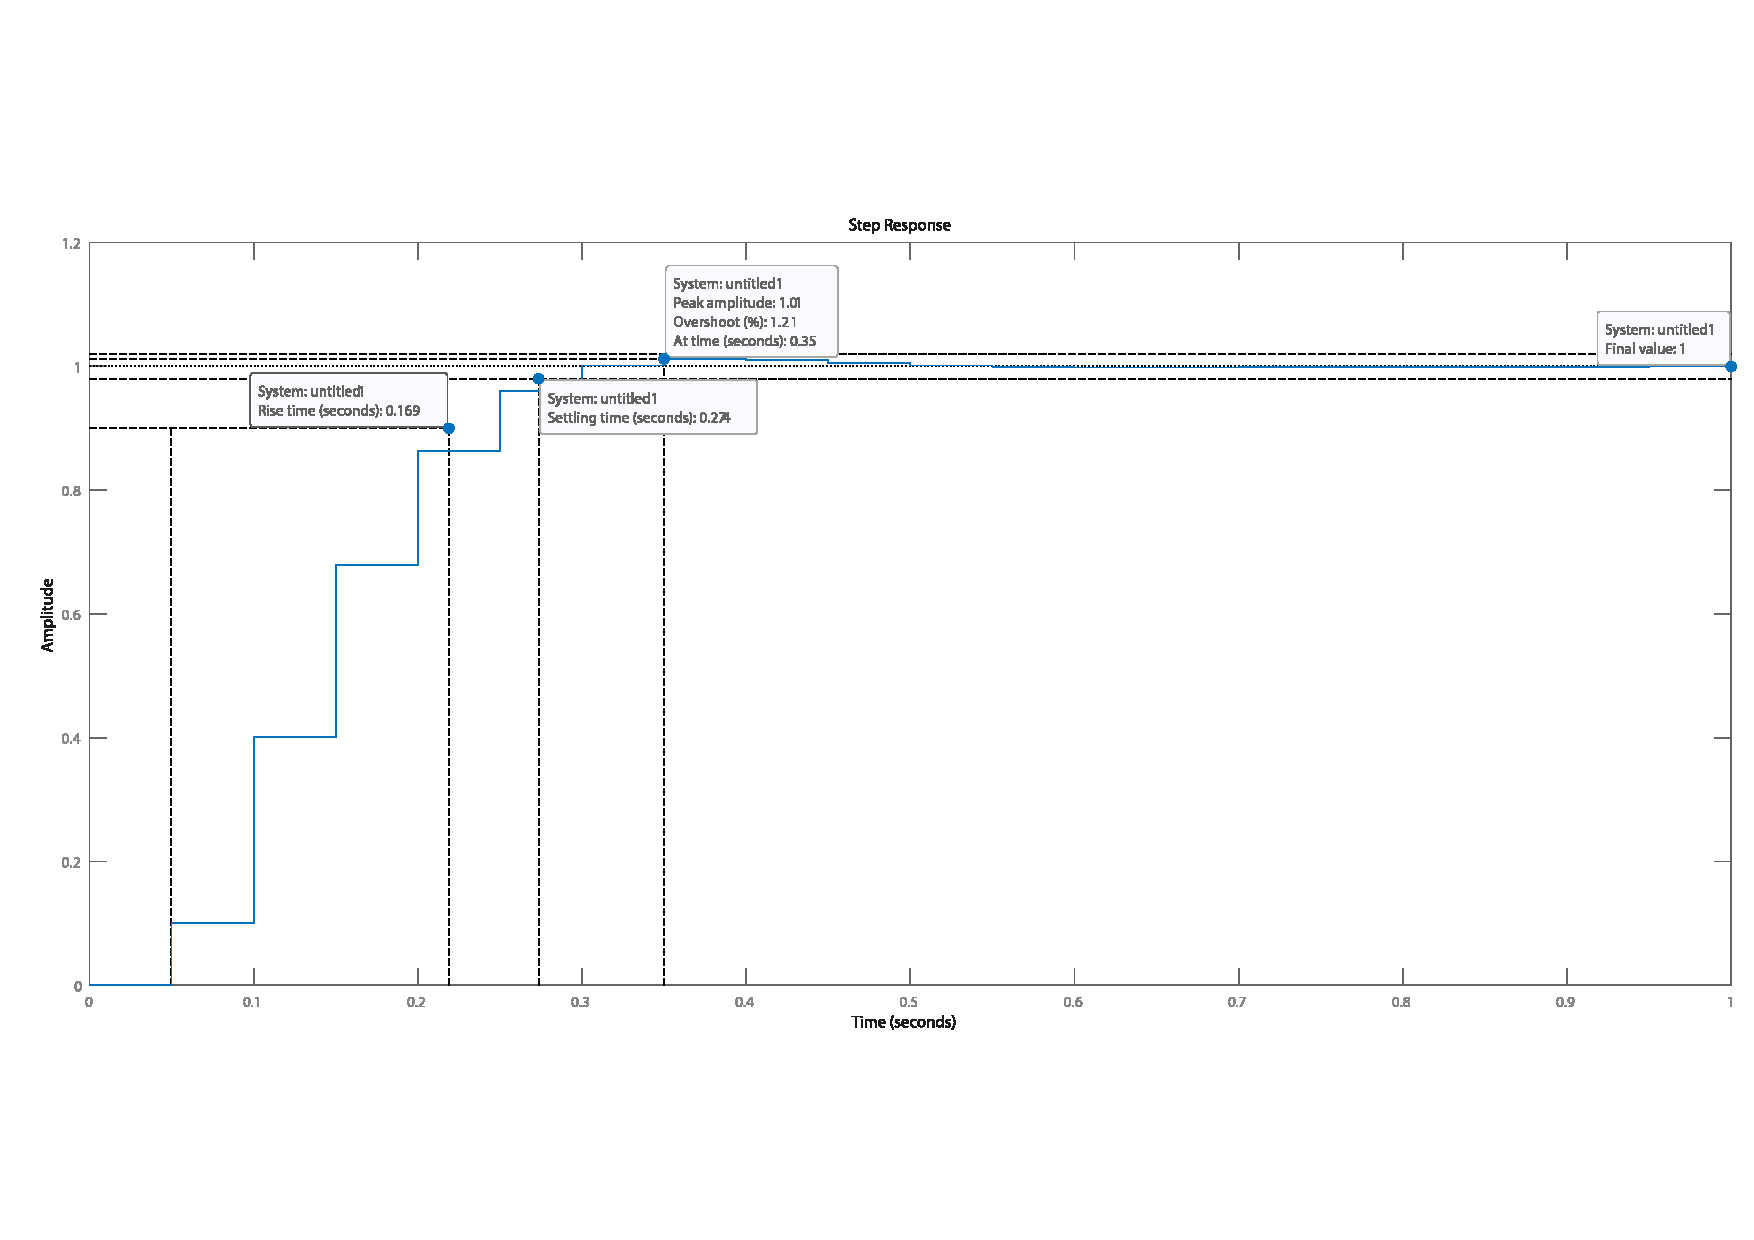
\includegraphics[clip, trim=0cm 3.6cm 0cm 3.7cm,scale=0.40]{images/figura 7.pdf}
  % izquierda,abajo,derecha,arriba
  \caption{Respuesa del sistema frente a un escalón con un controlador PD.}
    \label{fig:figura 7}
\end{figure}
}

\end{tcolorbox}%
\newpage
\subsection{Actividad 10}
Repetir el apartado anterior realizando un diseño de controlador
PID discreto implementable (PD, PI o PID) y ver si es posible cumplir
las especificaciones de sobreoscilación $< 10 \%$, tiempo de
establecimiento test $< 1 s$, error nulo ante ángulo de consigna
escalón unitario y error nulo ante ángulo de consigna rampa unitaria,
graficando la respuesta escalón y rampa, graficando el nuevo lugar de
las raíces en $z$, y comprobando a través de \textsc{ltiview} que se
cumplen ciertamente las especificaciones requeridas.

\begin{tcolorbox}[sharp corners, colframe=bluebox, title= Controlador
  PID con sobreoscilamiento $< 10\%$ y $t_{est} < 1$.,breakable=unlimited]
  $>>>$ rltool(Gposicionz)\\
  \vspace*{0.35em}
  \mkanscode{
\begin{figure}[H]
  \centering
  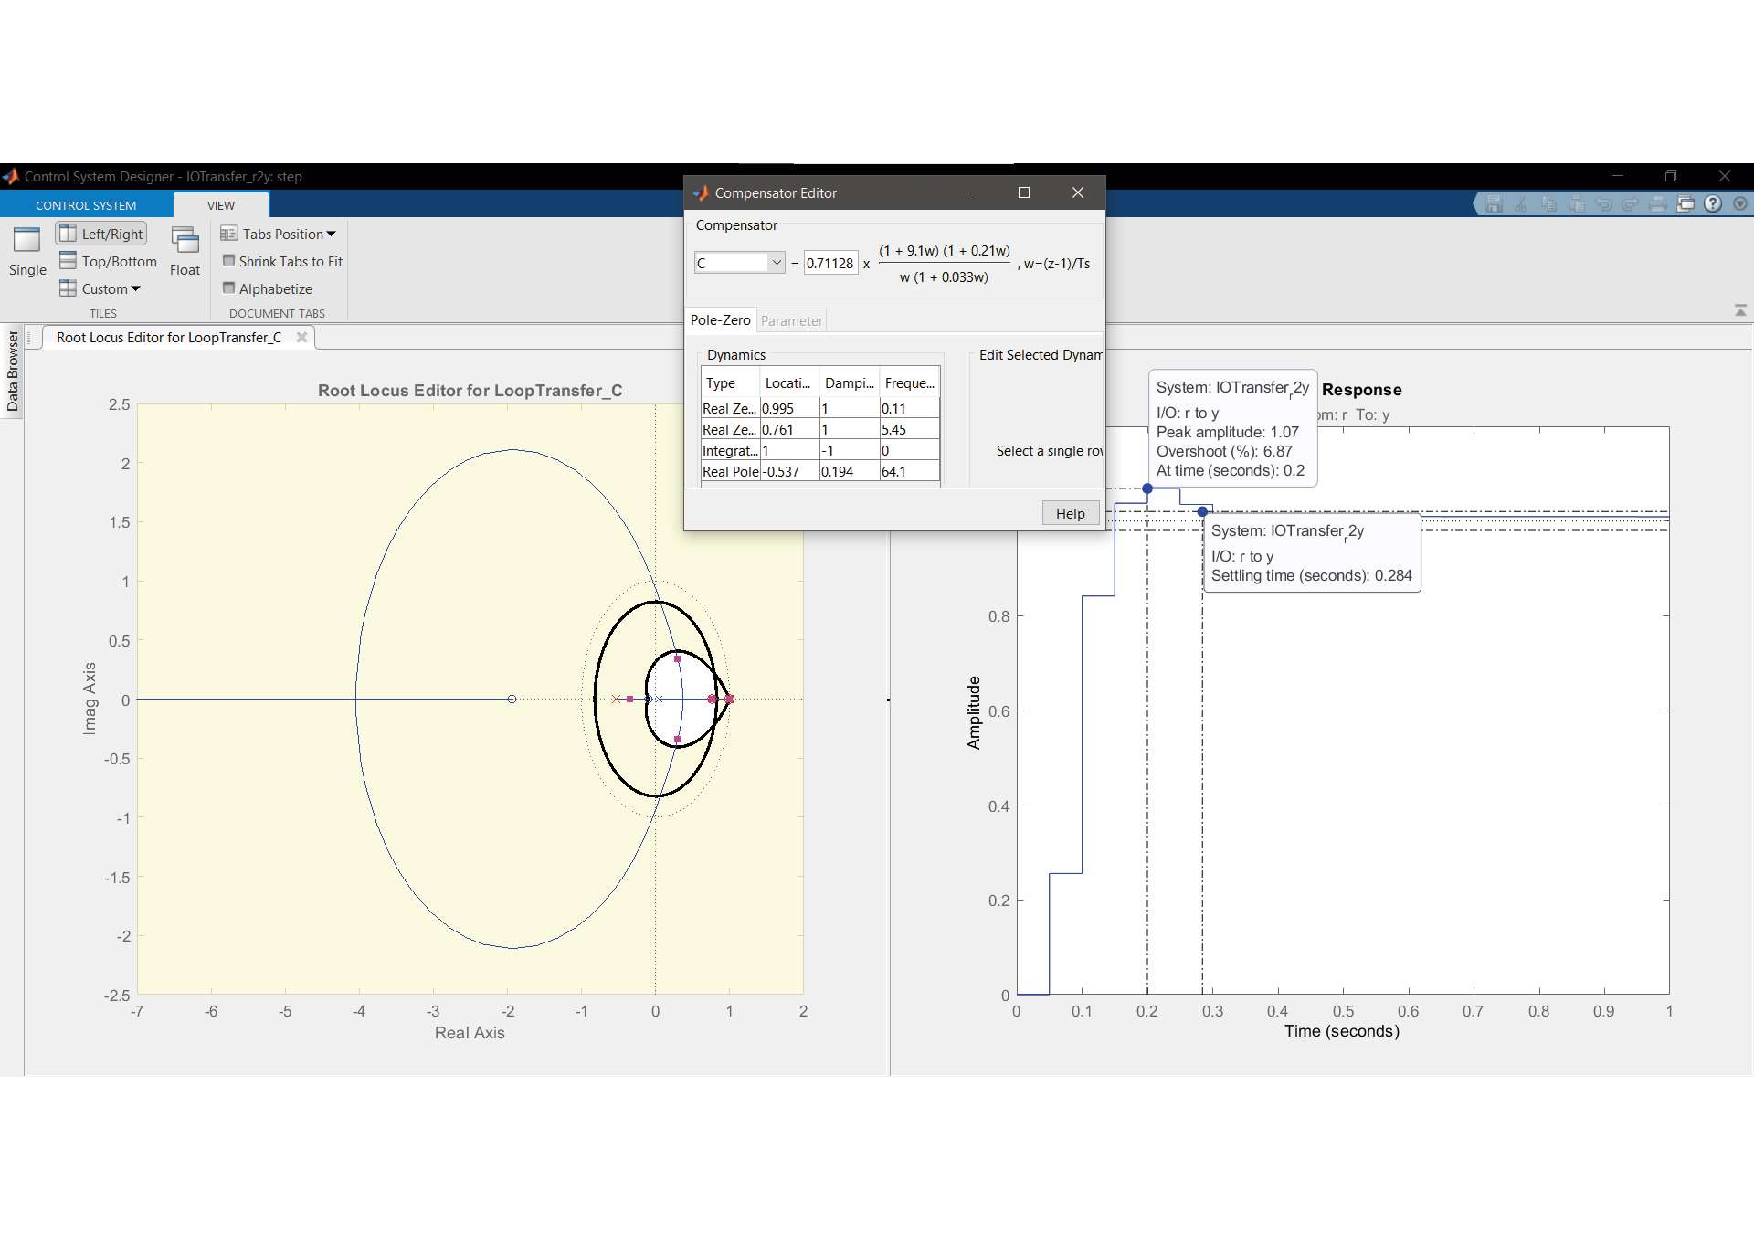
\includegraphics[clip, trim=0cm 2.5cm 0cm 2.5cm,
  scale=0.45]{images/figura 8.pdf}
  % izquierda,abajo,derecha,arriba
  \caption{Controlador PID.}
    \label{fig:figura 8}
\end{figure}
}
\vspace*{0.35em}
Mediante la herramienta \textsc{Export>Export tuned blocks.} podemos
enviar el controlador al espacio de trabajo.

$>>>$ PID\_10
\vspace*{0.35em}
\begin{tcolorbox}[sharp corners, colback = white]
    \color{gray}
\begin{verbatim}
PID_10 =
 
  41.625 (z-0.9945) (z-0.7613)
  ----------------------------
        (z-1) (z+0.5366)
 
Sample time: 0.05 seconds
Discrete-time zero/pole/gain model.
\end{verbatim}
  \end{tcolorbox}%
  \vspace*{0.5em}
\end{tcolorbox}%

\begin{tcolorbox}[sharp corners, colframe=bluebox, title= Respuesta
  del sistema en tiempo discreto con un controlador PID.]
  $>>>$ ltiview(\textcolor{blue}{`step'},kr*feedback(PID\_10*Gposicionz,kr))
  \vspace*{0.35em}
  \mkanscode{
\begin{figure}[H]
  \centering
  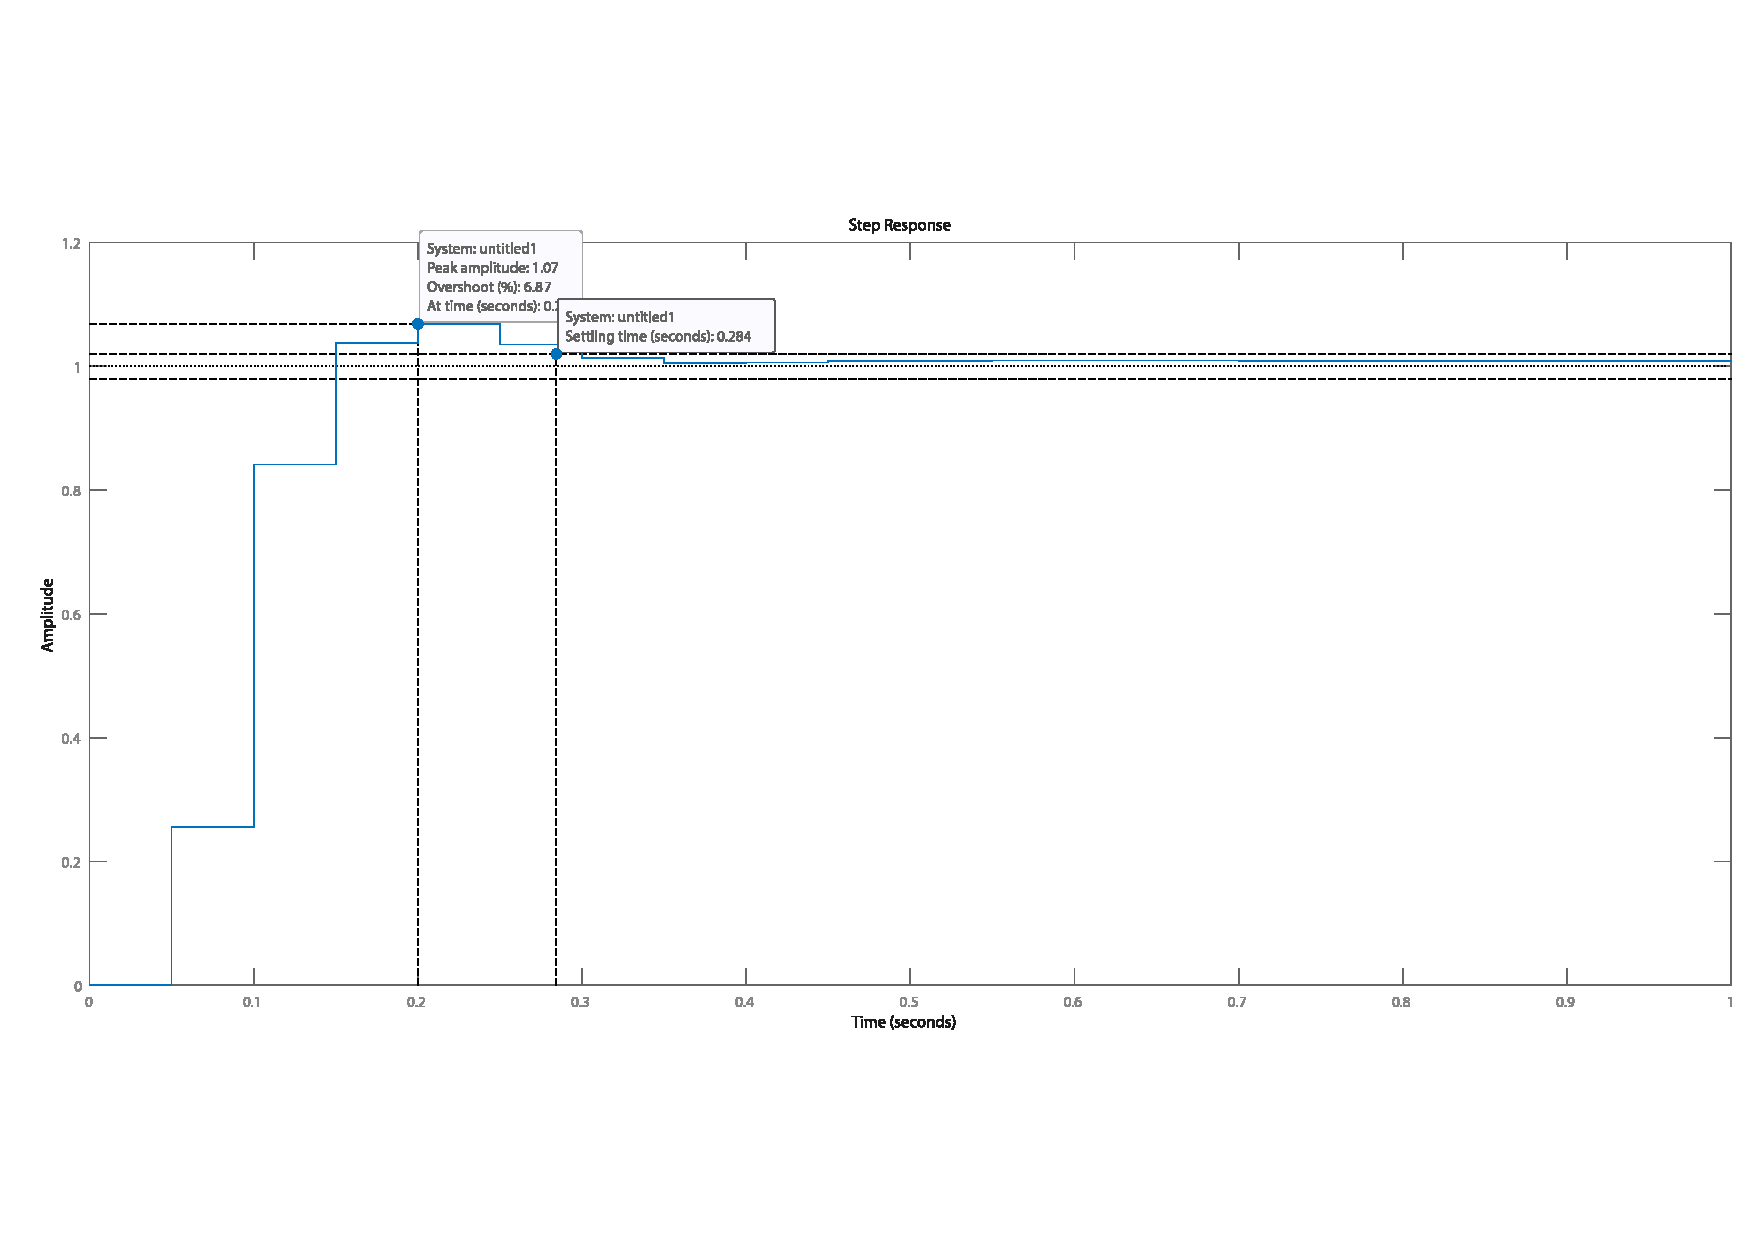
\includegraphics[clip, trim=0cm 3.6cm 0cm 3.4cm,scale=0.45]{images/figura 9.pdf}
  % izquierda,abajo,derecha,arriba
  \caption{Respuesa del sistema frente a un escalón con un controlador PID.}
    \label{fig:figura 9}
\end{figure}
}

\end{tcolorbox}%

\begin{tcolorbox}[sharp corners, colframe=bluebox, title= Respuesta
  del sistema en tiempo discreto con un controlador PID.]
  $>>>$ ltiview(\textcolor{blue}{`lsim'},kr*feedback(PID\_10*Gposicionz,kr))
  \vspace*{0.35em}
  \mkanscode{
\begin{figure}[H]
  \centering
  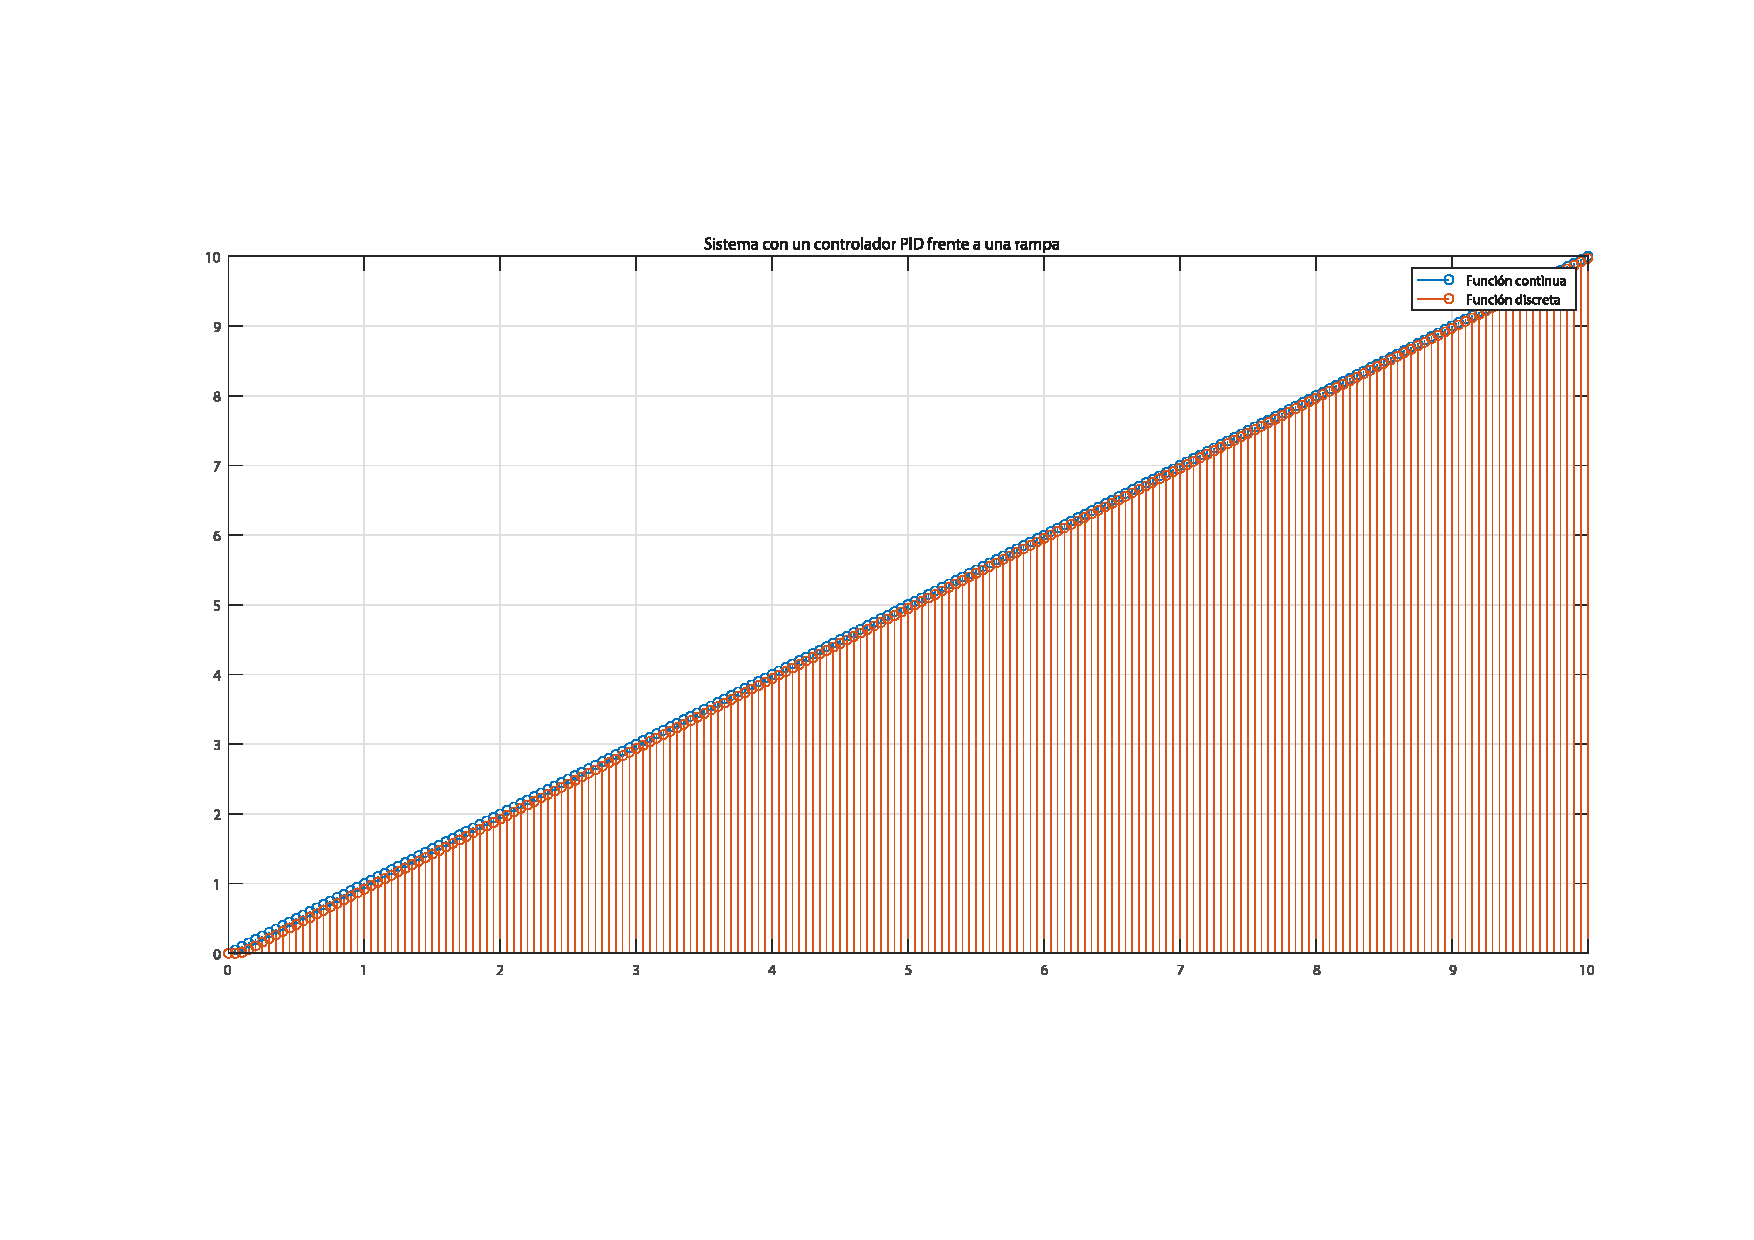
\includegraphics[clip, trim=2cm 3.6cm 1.4cm 3.4cm,scale=0.48]{images/figura 10.pdf}
  % izquierda,abajo,derecha,arriba
  \caption{Respuesa del sistema frente a una rampa con un controlador PID.}
    \label{fig:figura 10}
\end{figure}
}

\end{tcolorbox}%
\subsection{Actividad 11}
Simular en \textsc{SIMULINK} los sistemas de control PID
discreto de los apartados 9. y 10. usando los parámetros
correspondientes, añadiendo asimismo una limitación de salida del
controlador discreto a $(-15,+15)$ añadiendo en su caso el sistema
corrector anti-windup y ver la respuesta ante ángulo de consigna
escalón unitaria, graficando asimismo la señal de control.

\begin{tcolorbox}[sharp corners, colframe=bluebox, title= Simulink PD]
  \mkanscode{
\begin{figure}[H]
  \centering
  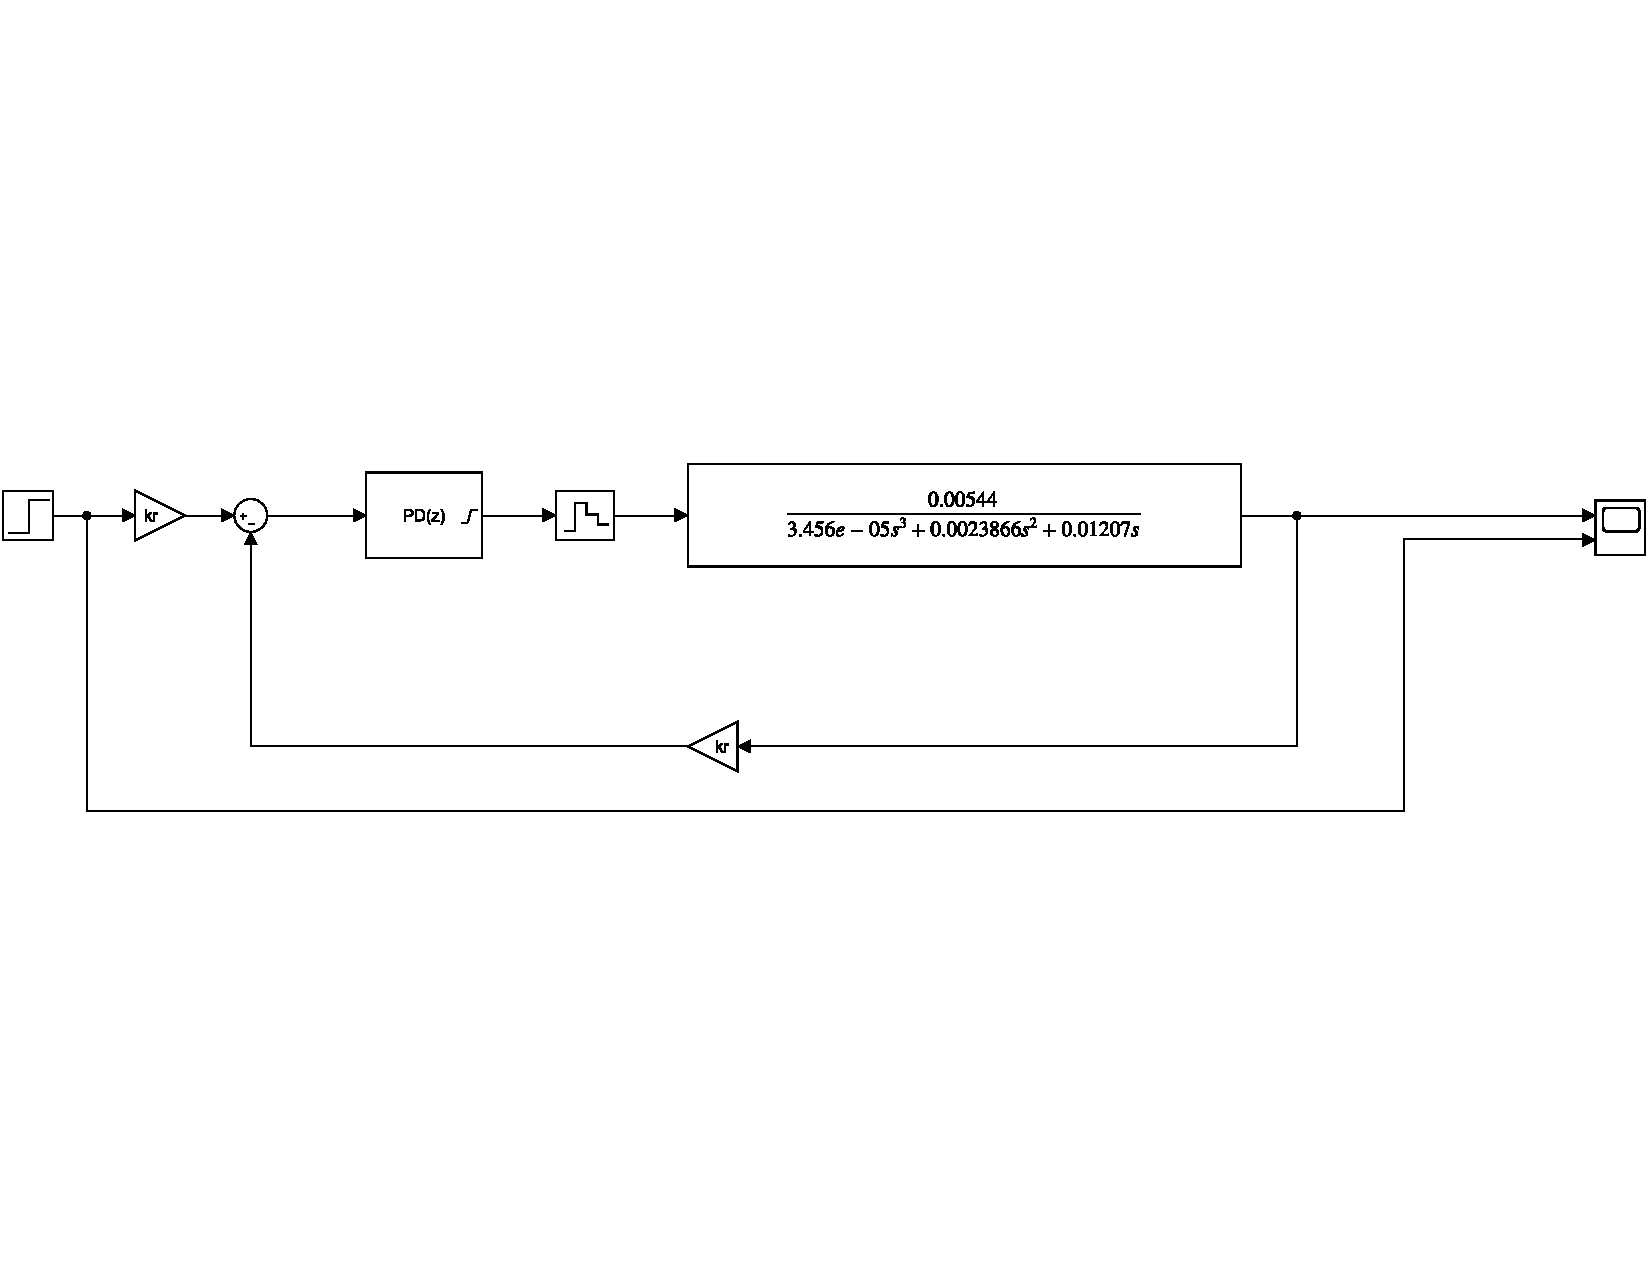
\includegraphics[clip, trim=0cm 6cm 0cm 6cm,scale=0.48]{images/figura 11.pdf}
  % izquierda,abajo,derecha,arriba
  \caption{Simulink - Diagrama de bloques.}
    \label{fig:figura 11}
\end{figure}
}

\begin{tcolorbox}[sharp corners, colback = white]
    \color{gray}
\begin{verbatim}
Use filtered derivative
    Filter coefficient (N): 45
Upper limit: 15
Lower limit: -15 
\end{verbatim}
  \end{tcolorbox}%
\vspace*{0.5em}
  \mkanscode{
\begin{figure}[H]
  \centering
  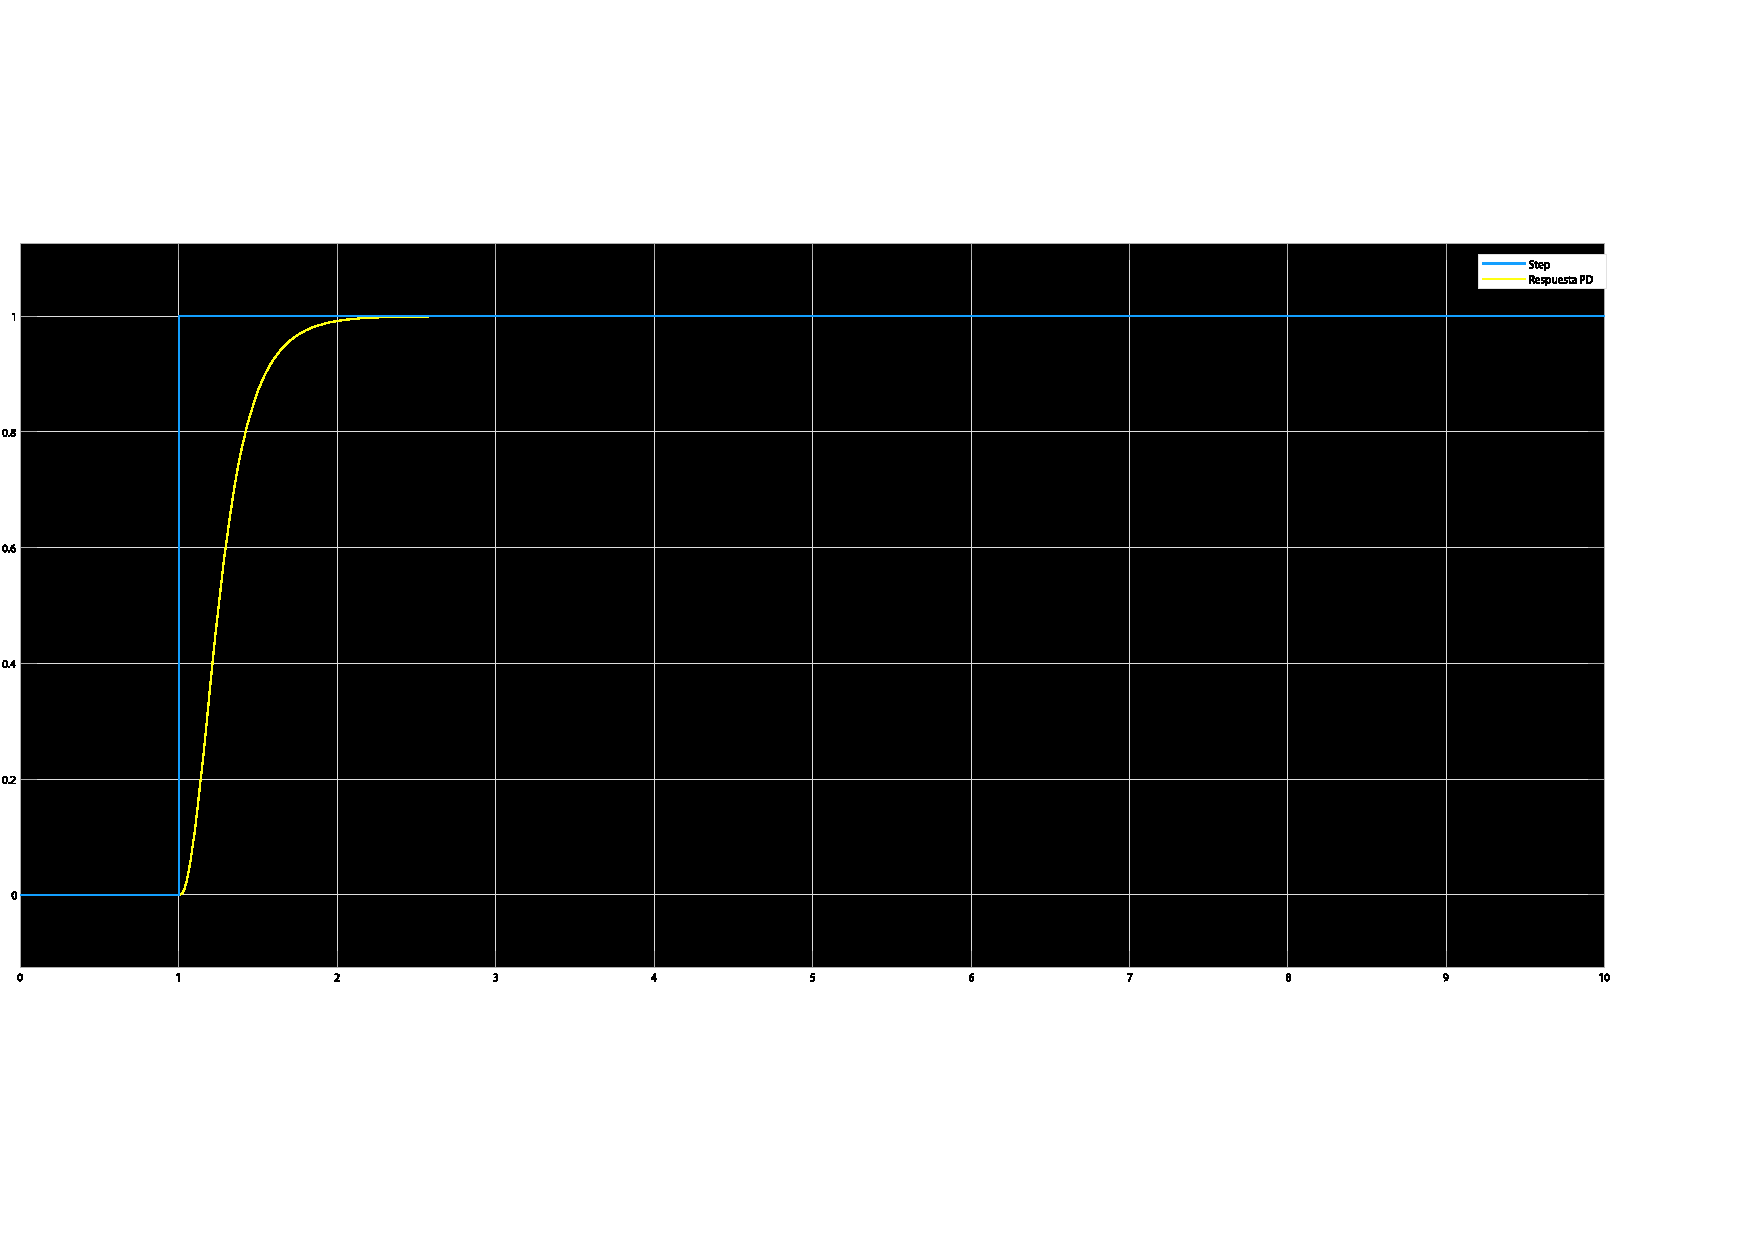
\includegraphics[clip, trim=0cm 4cm 0.90cm 4cm,scale=0.48]{images/figura 12.pdf}
  % izquierda,abajo,derecha,arriba
  \caption{Simulink - Respuesta a un escalón.}
    \label{fig:figura 12}
\end{figure}
  }
\end{tcolorbox}%

\begin{tcolorbox}[sharp corners, colframe=bluebox, title= Simulink PID,breakable=unlimited]
  \mkanscode{
\begin{figure}[H]
  \centering
  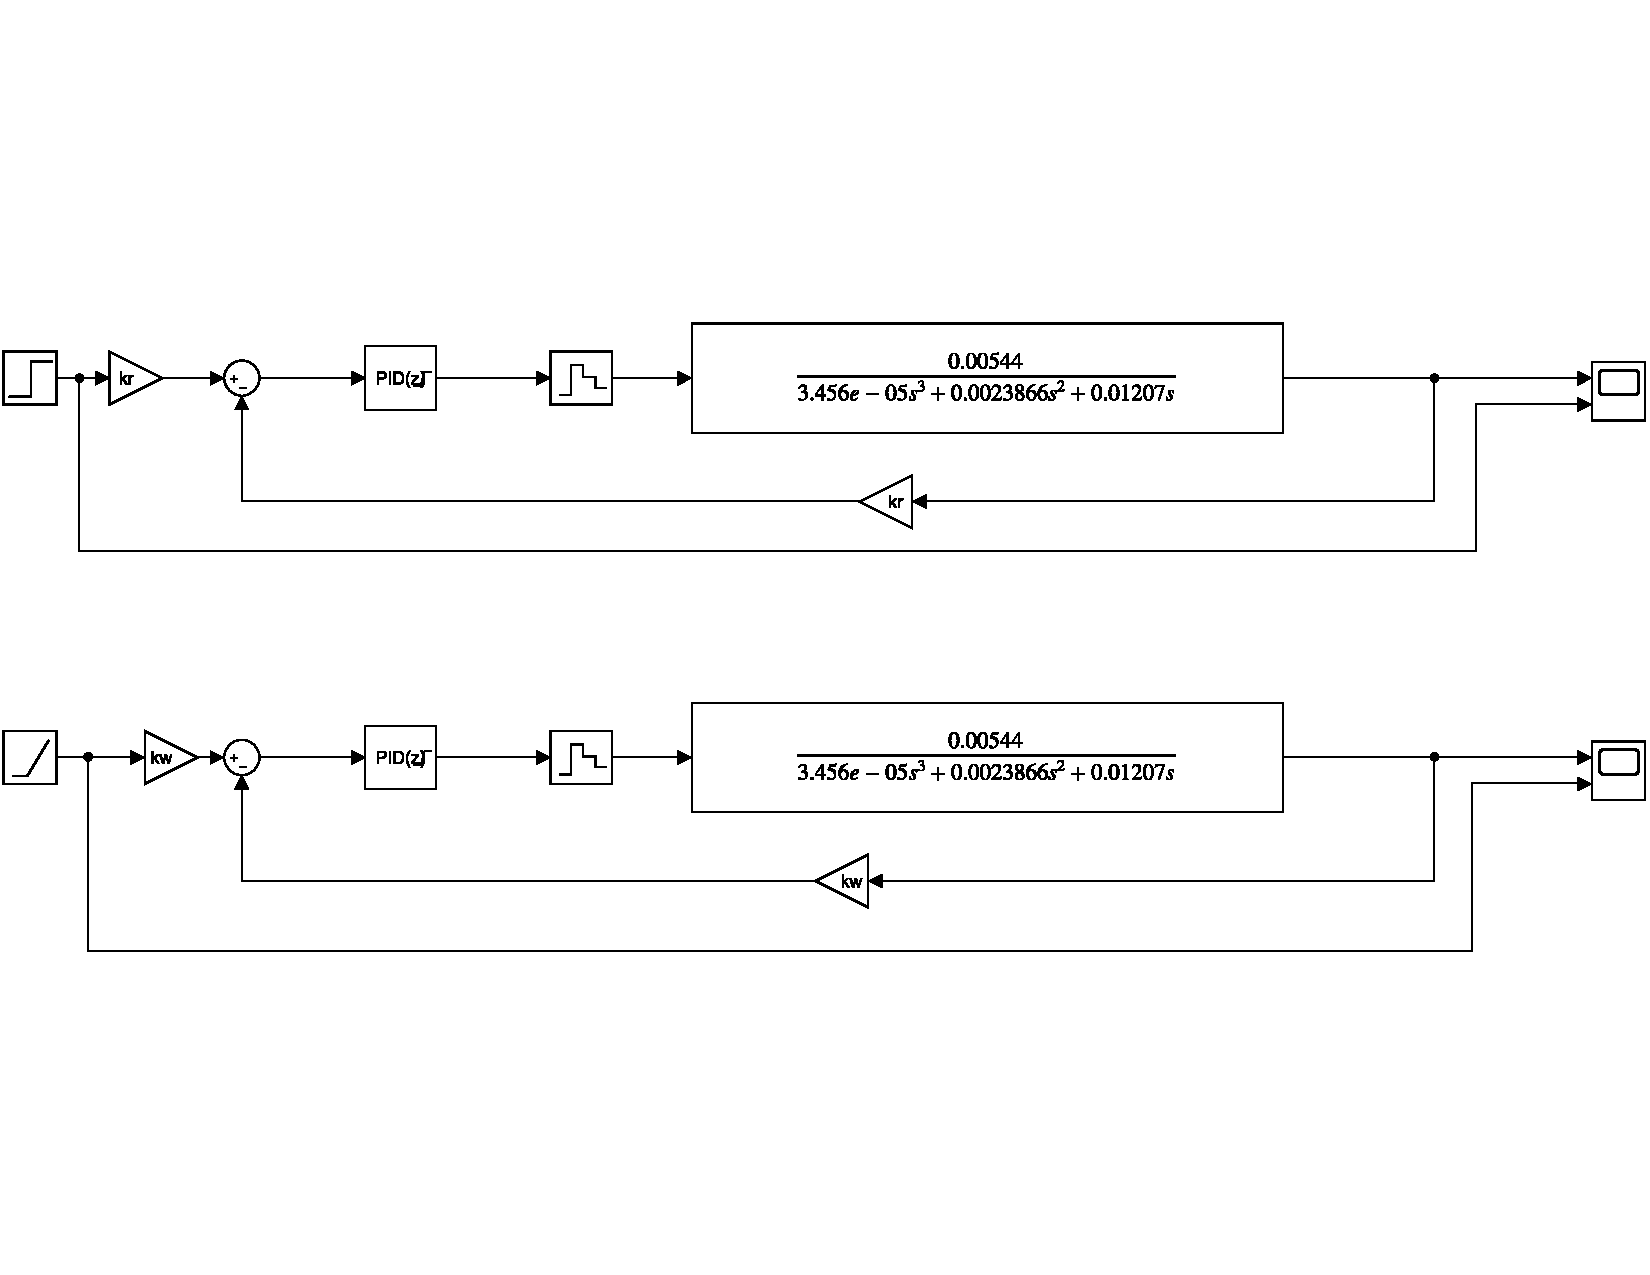
\includegraphics[clip, trim=0cm 5.35cm 0cm 5.34cm,scale=0.48]{images/figura 13.pdf}
  % izquierda,abajo,derecha,arriba
  \caption{Simulink - Diagrama de bloques.}
    \label{fig:figura 13}
\end{figure}
}

\begin{tcolorbox}[sharp corners, colback = white]
    \color{gray}
\begin{verbatim}
Use filtered derivative
    Filter coefficient (N): 45
Upper limit: 15
Lower limit: -15 
Anti-windup Method: Campling
\end{verbatim}
  \end{tcolorbox}%
\vspace*{0.5em}
  \mkanscode{
\begin{figure}[H]
  \centering
  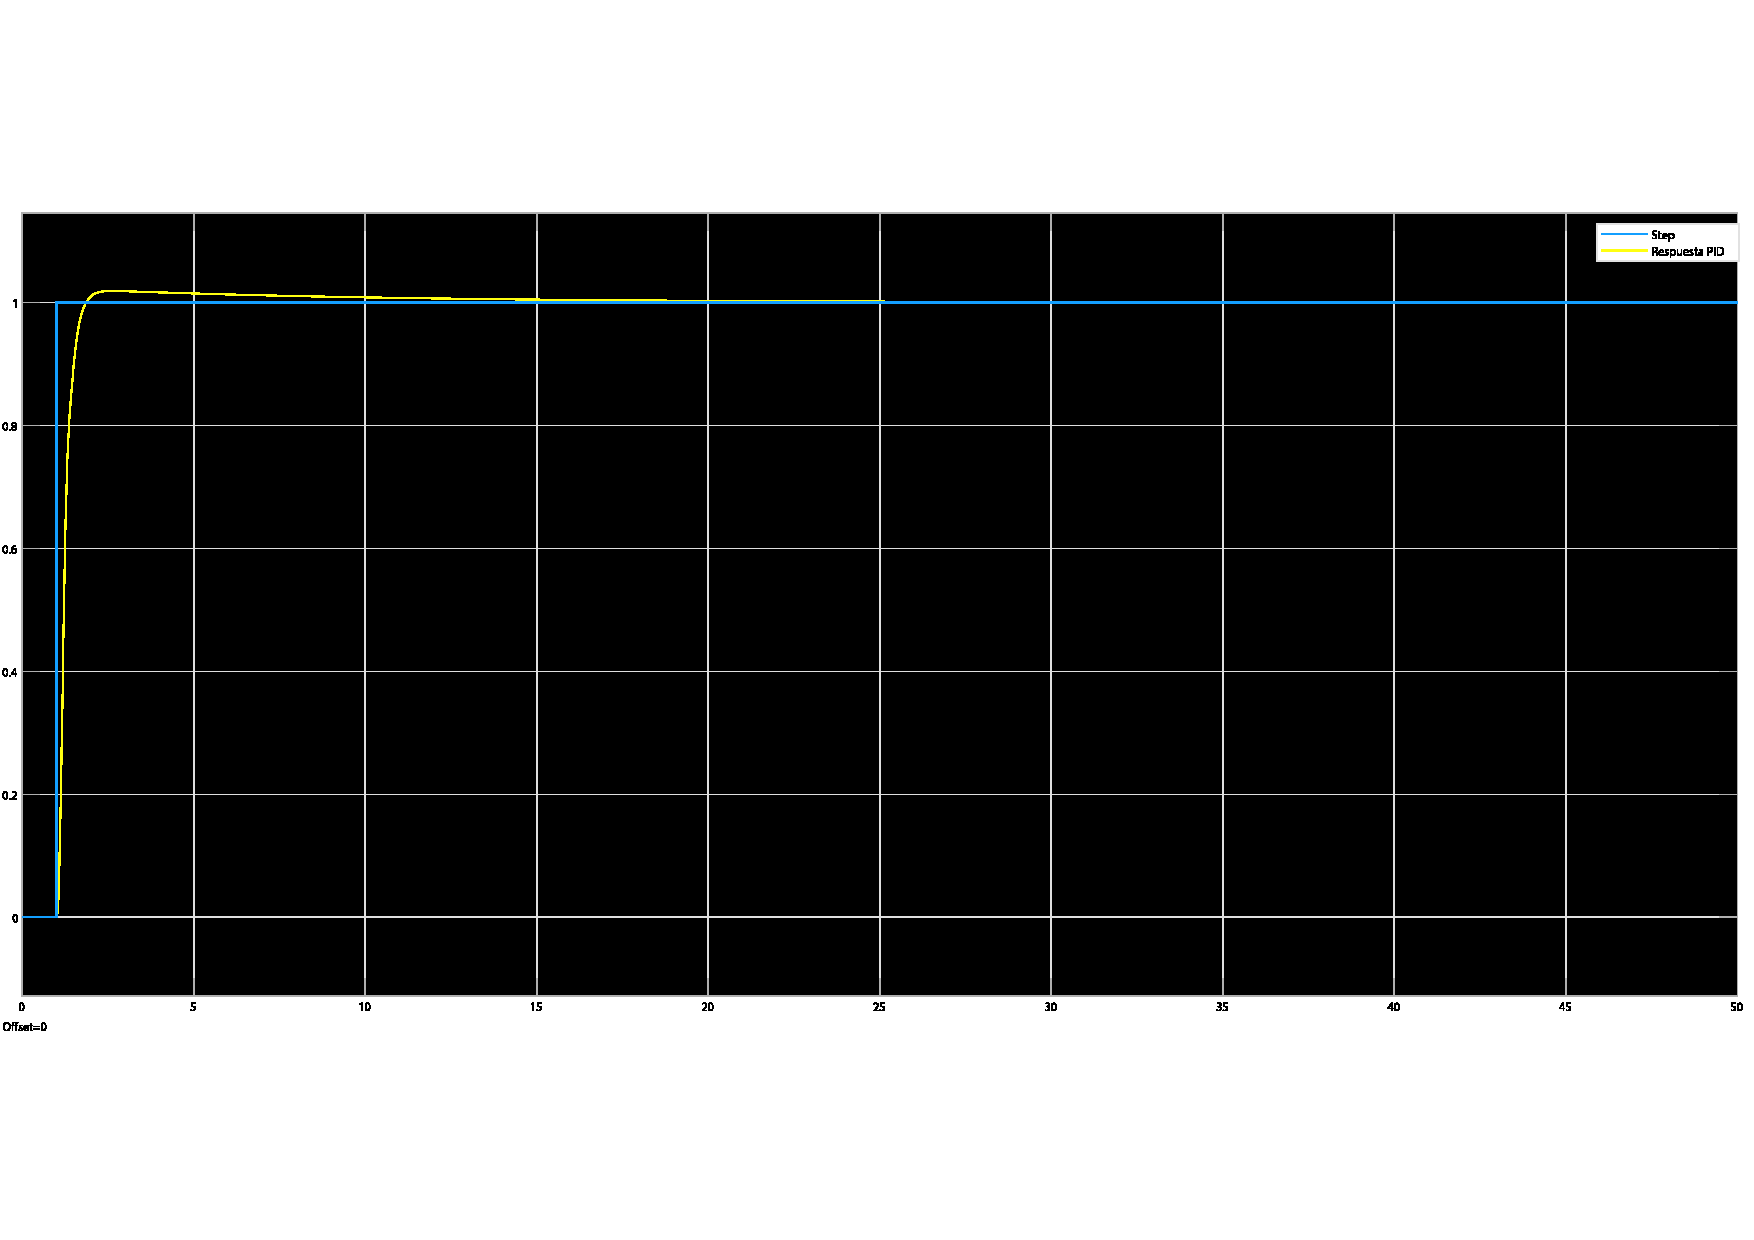
\includegraphics[clip, trim=0cm 3.7cm 0cm 3.7cm,scale=0.48]{images/figura 14.pdf}
  % izquierda,abajo,derecha,arriba
  \caption{Simulink - Respuesta a un escalón.}
    \label{fig:figura 14}
\end{figure}
}
\vspace*{0.5em}
  \mkanscode{
\begin{figure}[H]
  \centering
  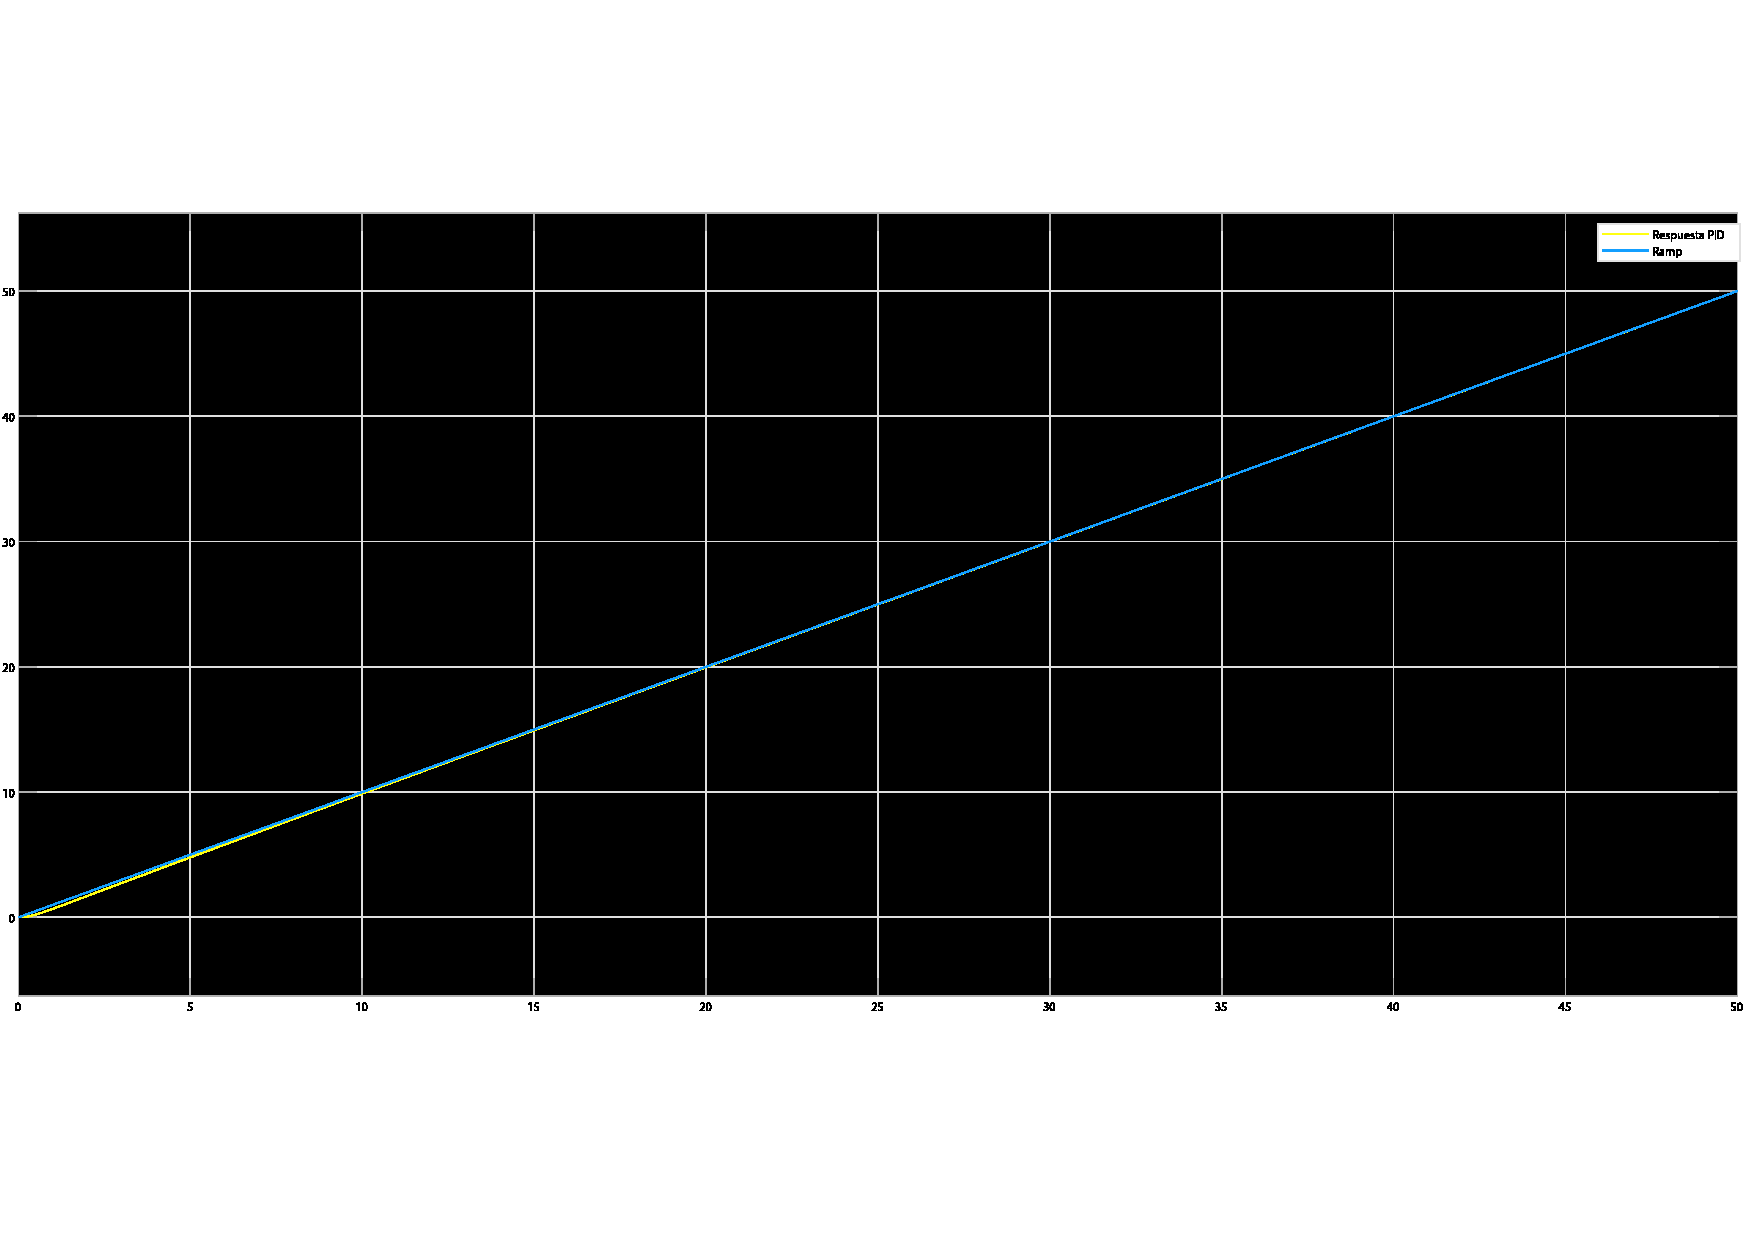
\includegraphics[clip, trim=0cm 3.7cm 0cm 3.7cm,scale=0.48]{images/figura 15.pdf}
  % izquierda,abajo,derecha,arriba
  \caption{Simulink - Respuesta a una rampa.}
    \label{fig:figura 15}
\end{figure}
  }
  \end{tcolorbox}%
\newpage
\subsection{Actividad 12}
Resintonizar el controlador digital respectivamente en
\textsc{SIMULINK} a través de las herramientas de diseño automático,
obteniendo una mejora en la respuesta posible ante seguimiento de
consigna ángulo de amplitud unitaria.

\begin{tcolorbox}[sharp corners, colframe=bluebox, title= Simulink]
  \mkanscode{
\begin{figure}[H]
  \centering
  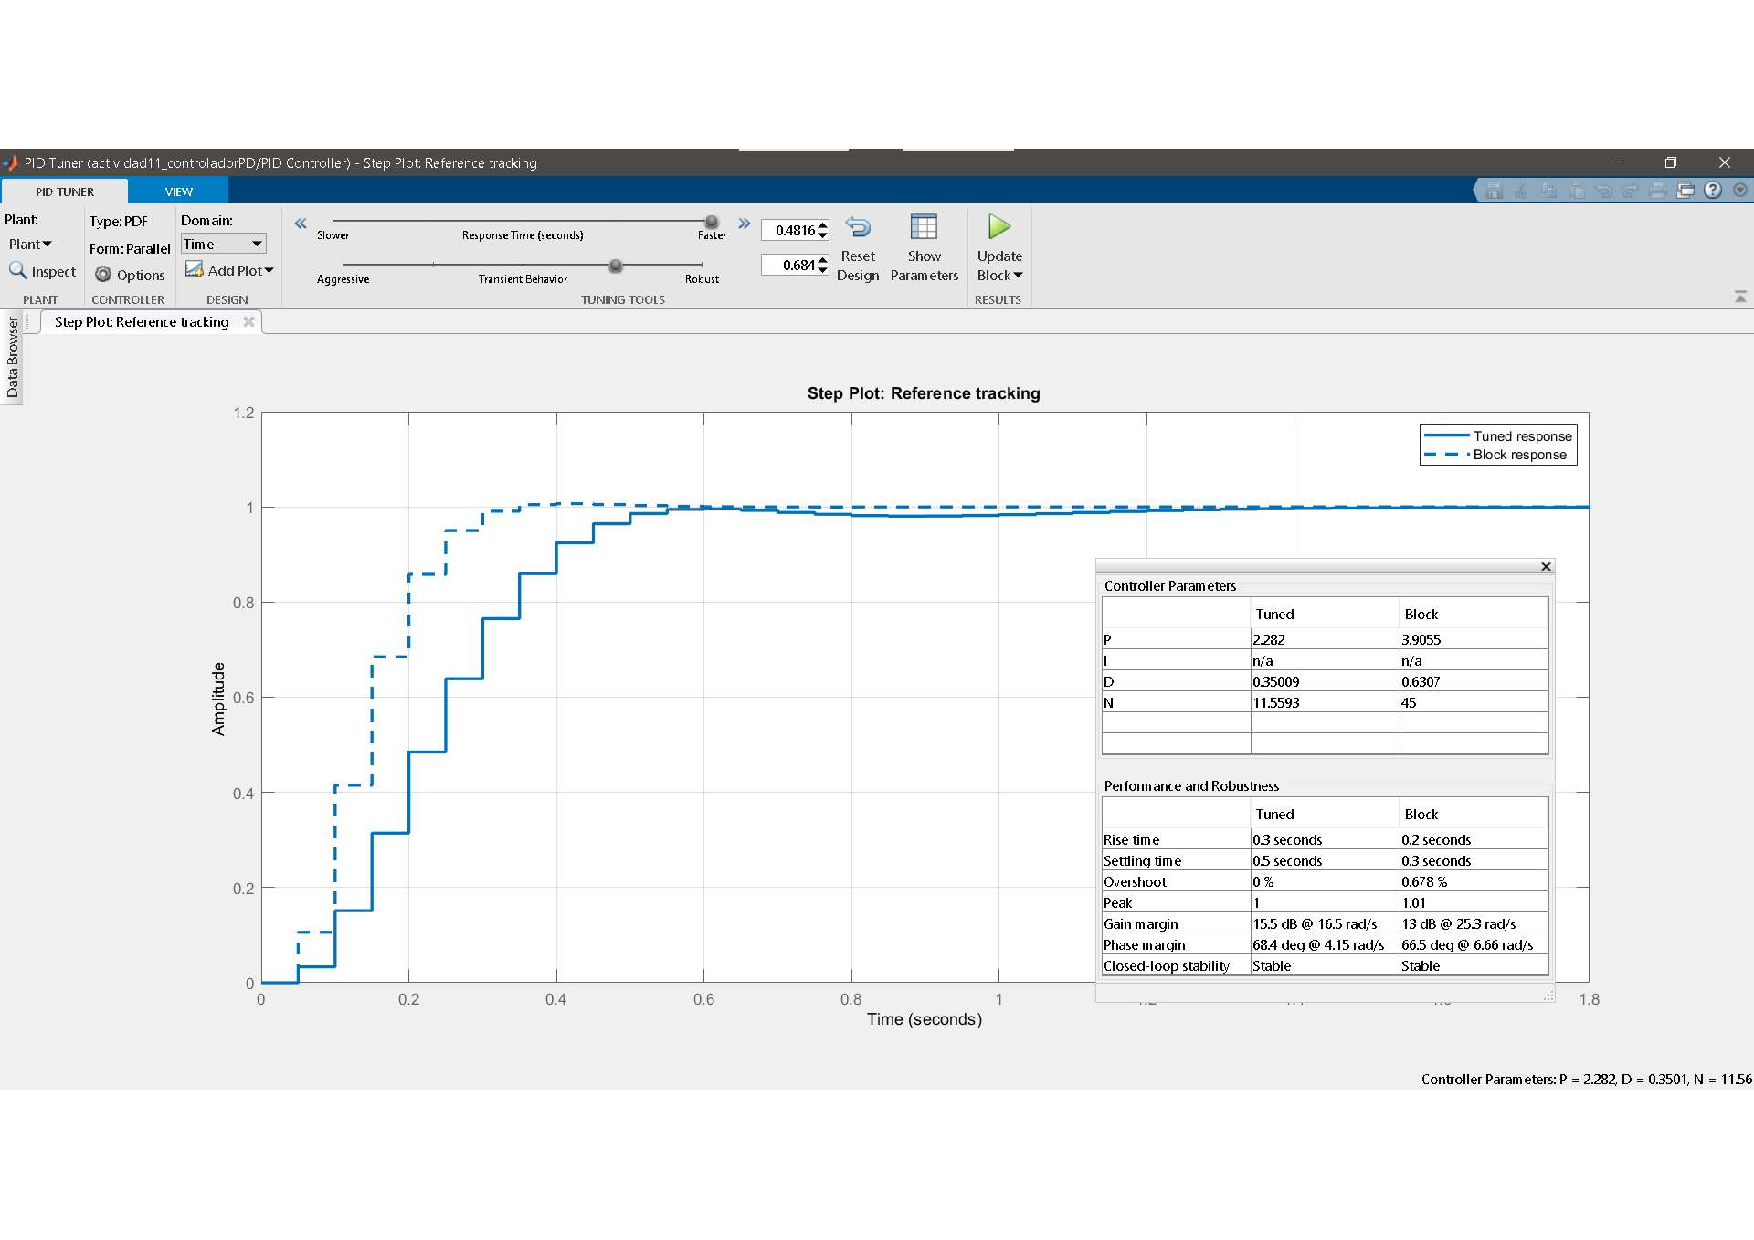
\includegraphics[clip, trim=0cm 2.5cm 0cm 2.5cm,scale=0.45]{images/figura 16.pdf}
  % izquierda,abajo,derecha,arriba
  \caption{Simulink Resintonización PD.}
    \label{fig:figura 16}
\end{figure}
}
\vspace*{0.5em}
  \mkanscode{
\begin{figure}[H]
  \centering
  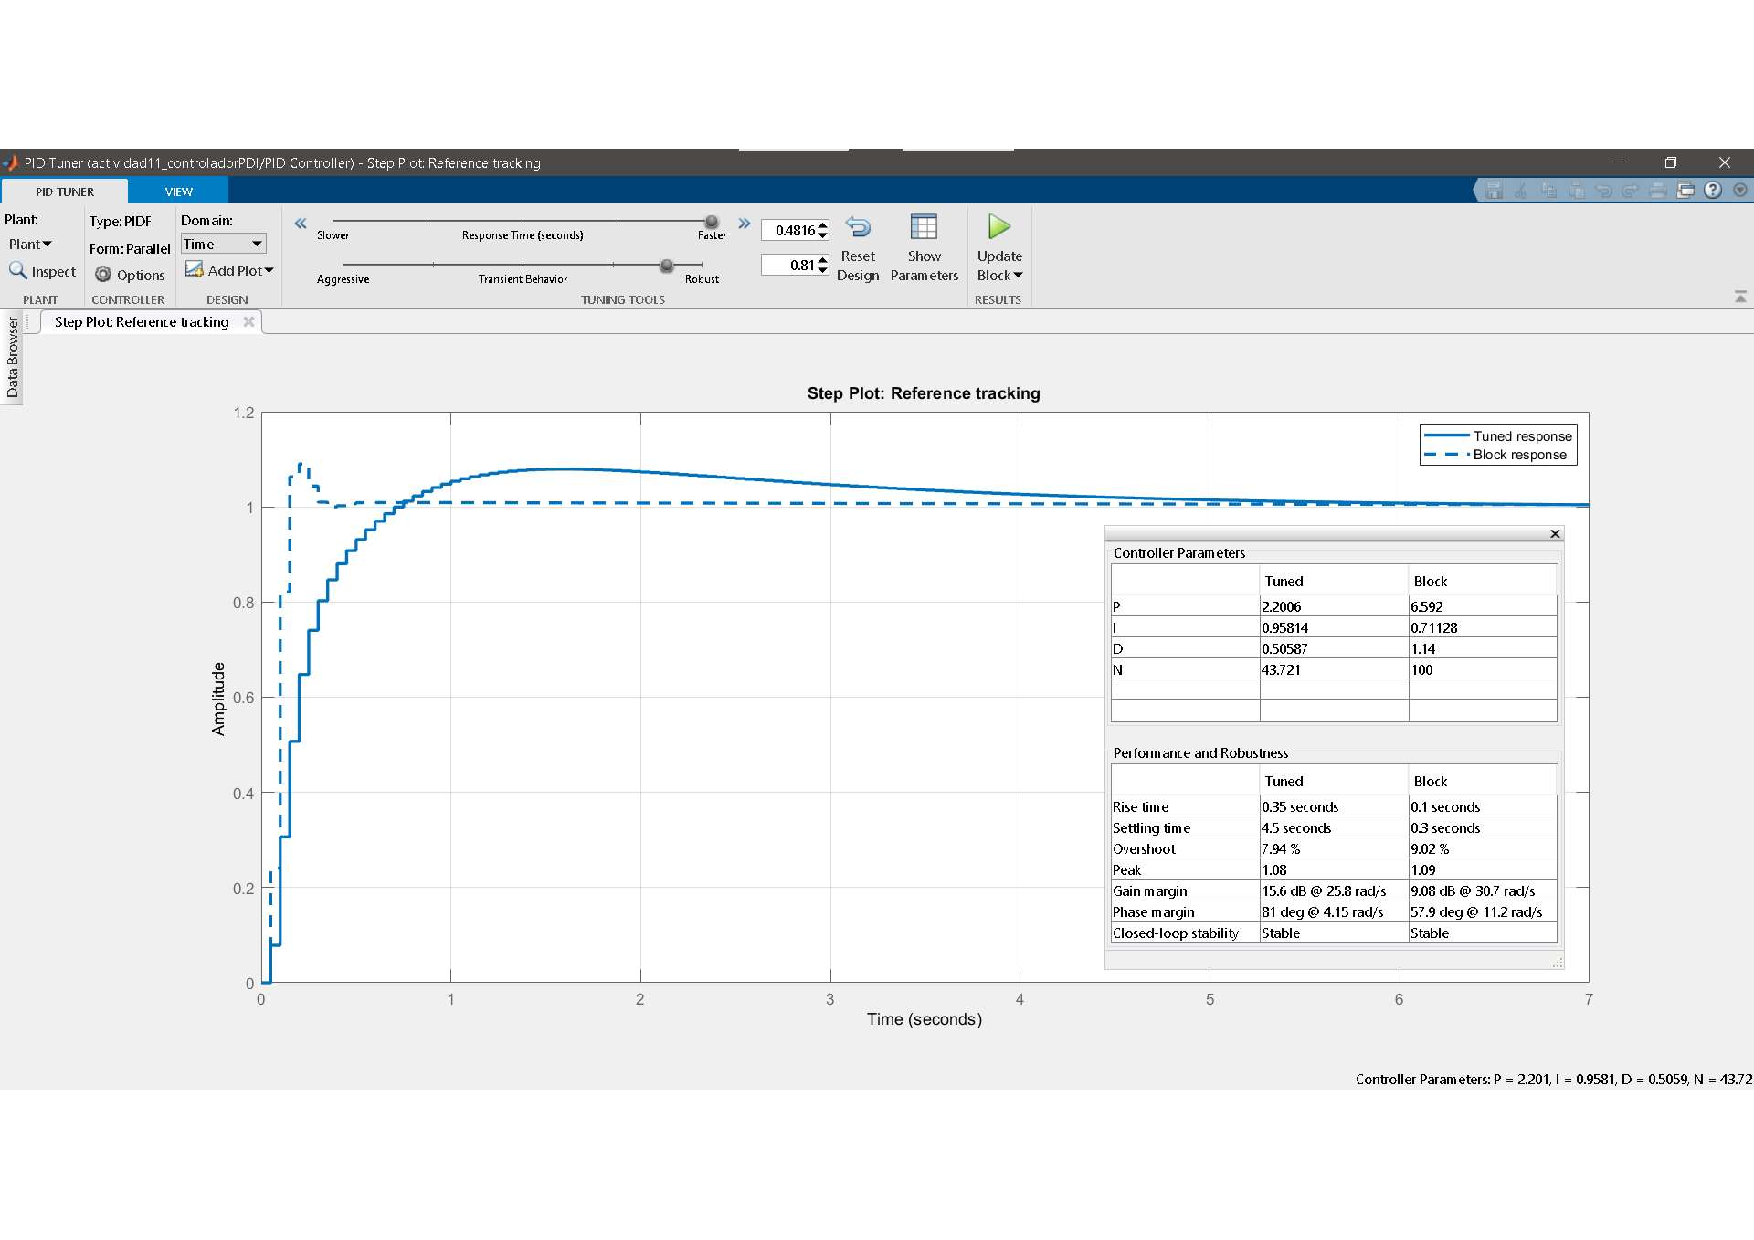
\includegraphics[clip, trim=0cm 2.5cm 0cm 2.5cm,scale=0.45]{images/figura 17.pdf}
  % izquierda,abajo,derecha,arriba
  \caption{Simulink Resintonización PID.}
    \label{fig:figura 17}
\end{figure}
  }
  \end{tcolorbox}%
\newpage
\subsection{Actividad 13}
Diseñar un controlador analógico tipo PID (PD, PI, PID) para el
sistema servomotor de posición por el \textsc{método de
Ziegler-Nichols} en abierto y cerrado (si son posibles) y realizar su
discretizacion con $T=0.05$ aplicando el método trapezoidal y graficar
la respuesta escalón unitaria del sistema de control en bucle cerrado
del servomotor de posición a través de la herramienta \textsc{rltool}.

Para implementar el método Ziegler-Nichols en bucle abierto,
necesitamos que la respuesta ante entrada escalón sea aproximadamente
la de un sistema de primer orden con retardo, por lo que no podemos
aplicar este método.  Por el contrario sí podemos implementar el
método Ziegler-Nichols en bucle cerrado.

\begin{tcolorbox}[sharp corners, colframe=bluebox, title= Método de
Ziegler-Nichols, breakable=unlimited]
 $>>>$ step(Gposicion)
  \vspace*{0.35em}
  \mkanscode{
\begin{figure}[H]
  \centering
  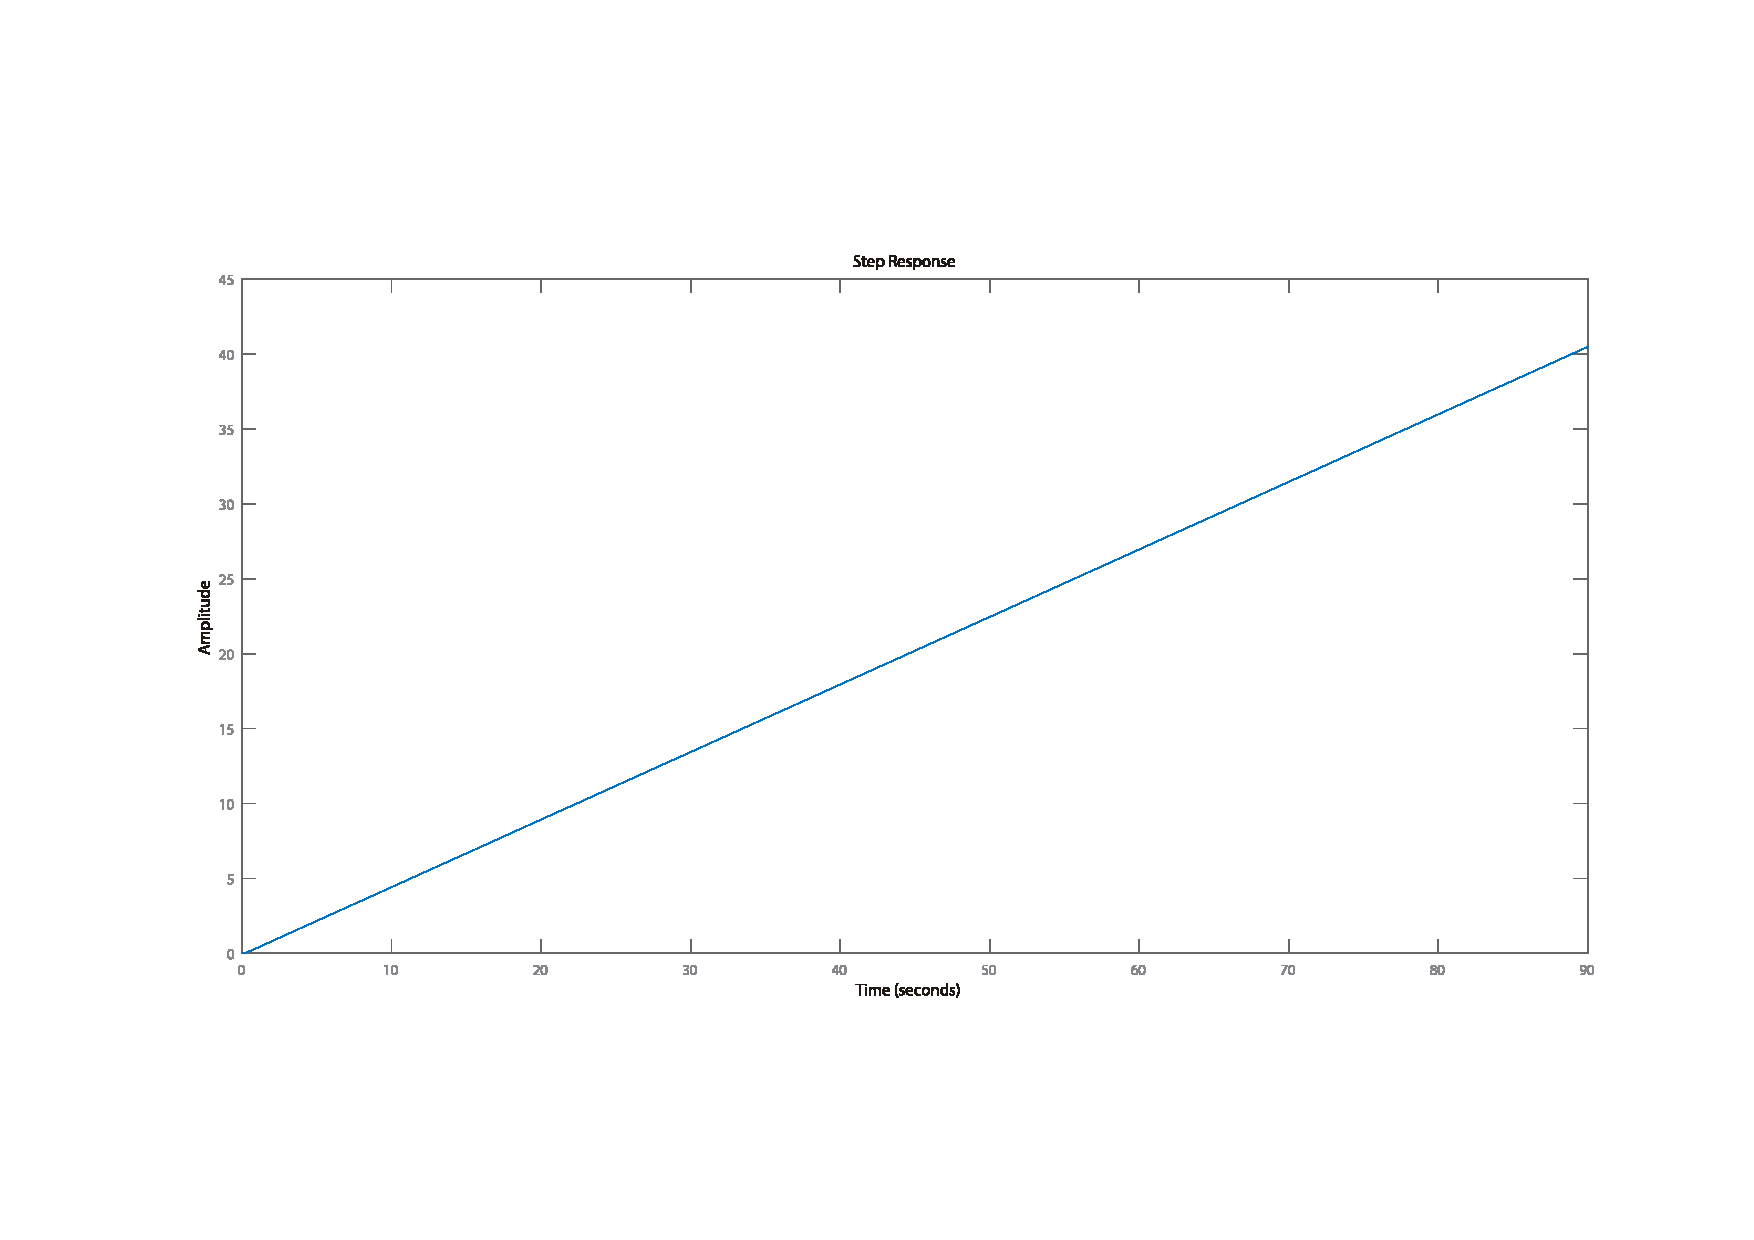
\includegraphics[clip, trim=2cm 3.6cm 1.4cm 3.4cm,scale=0.48]{images/figura 22.pdf}
  % izquierda,abajo,derecha,arriba
  \caption{Respuesta del sistema en bucle abierto frente a un escalón.}
    \label{fig:figura 22}
\end{figure}
}

Como es inestable no se puede hacer el PID Ziegler-Nichols en bucle
abierto, por lo tanto lo haremos en bucle cerrado.

$>>>$ [Kc,Pm,Wg]=margin(kr*Gposicion);\\
$>>>$ Tc = 2*pi/Wg;\\
$>>>$ Kp = 0.75*Kc;\\
$>>>$ Ti = Tc/1.6;\\
$>>>$ Ki = Kp/Ti;\\
$>>>$ Td = Tc/10;\\
$>>>$ Kd = Td*Kp;\\
$>>>$ tf = 0.01;\\
$>>>$ pidZN = pid(Kp,Ki,Kd,tf);\\
$>>>$ rltool(Gposicion,pidZN);\\
$>>>$ pidZNz = c2d(pidZN,T,'trapezoidal');\\
$>>>$ rltool(Gposicionz,pidZNz);\\

  \vspace*{0.35em}
  \mkanscode{
\begin{figure}[H]
  \centering
  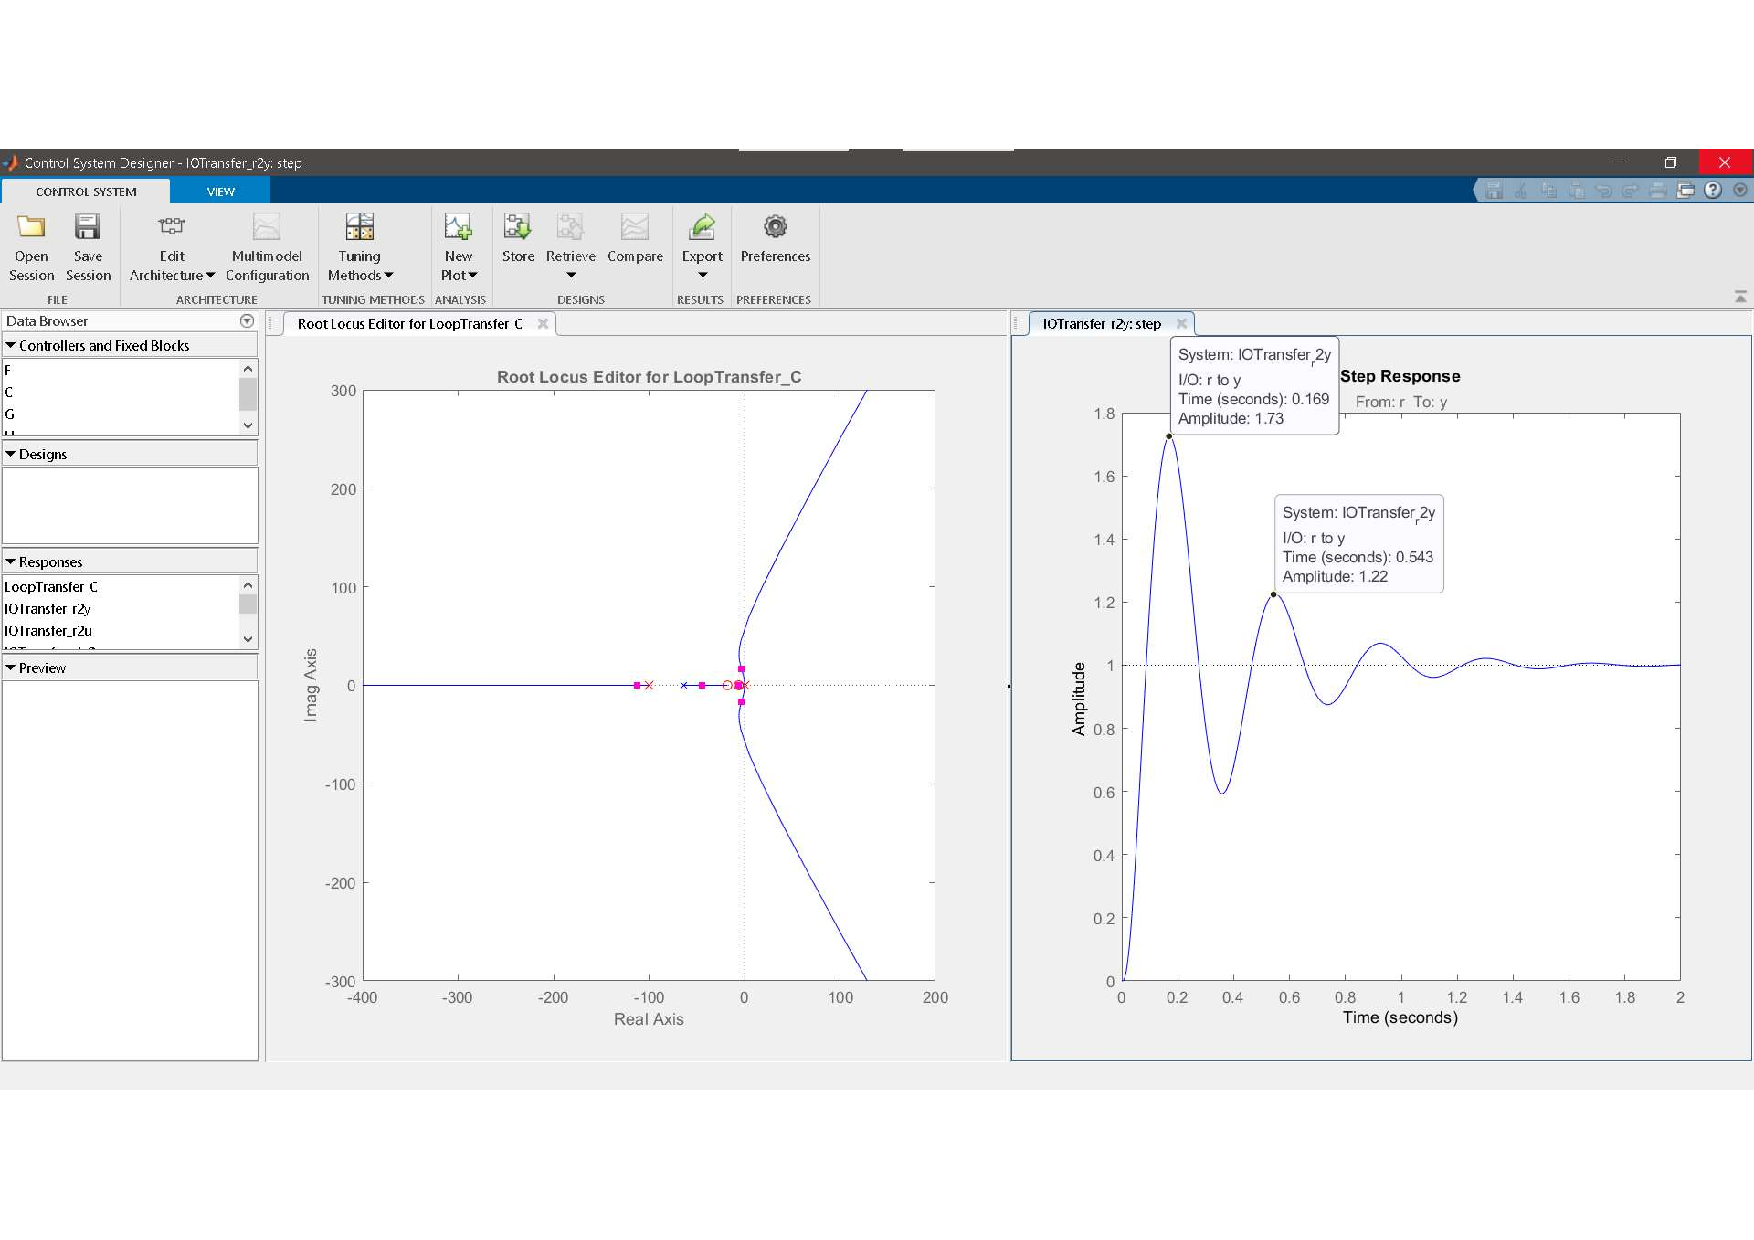
\includegraphics[clip, trim=0cm 3.5cm 0cm 2.8cm,scale=0.48]{images/figura 23.pdf}
  % izquierda,abajo,derecha,arriba
  \caption{Respuesta continua Ziegler-Nichols}
    \label{fig:figura 23}
\end{figure}
}
Calculamos la relación de sobreoscilación:\\
\begin{center}
  0.22/0.73 = 0.30 $\rightarrow$ 30\%
  \end{center}
  \vspace*{0.35em}
  \mkanscode{
\begin{figure}[H]
  \centering
  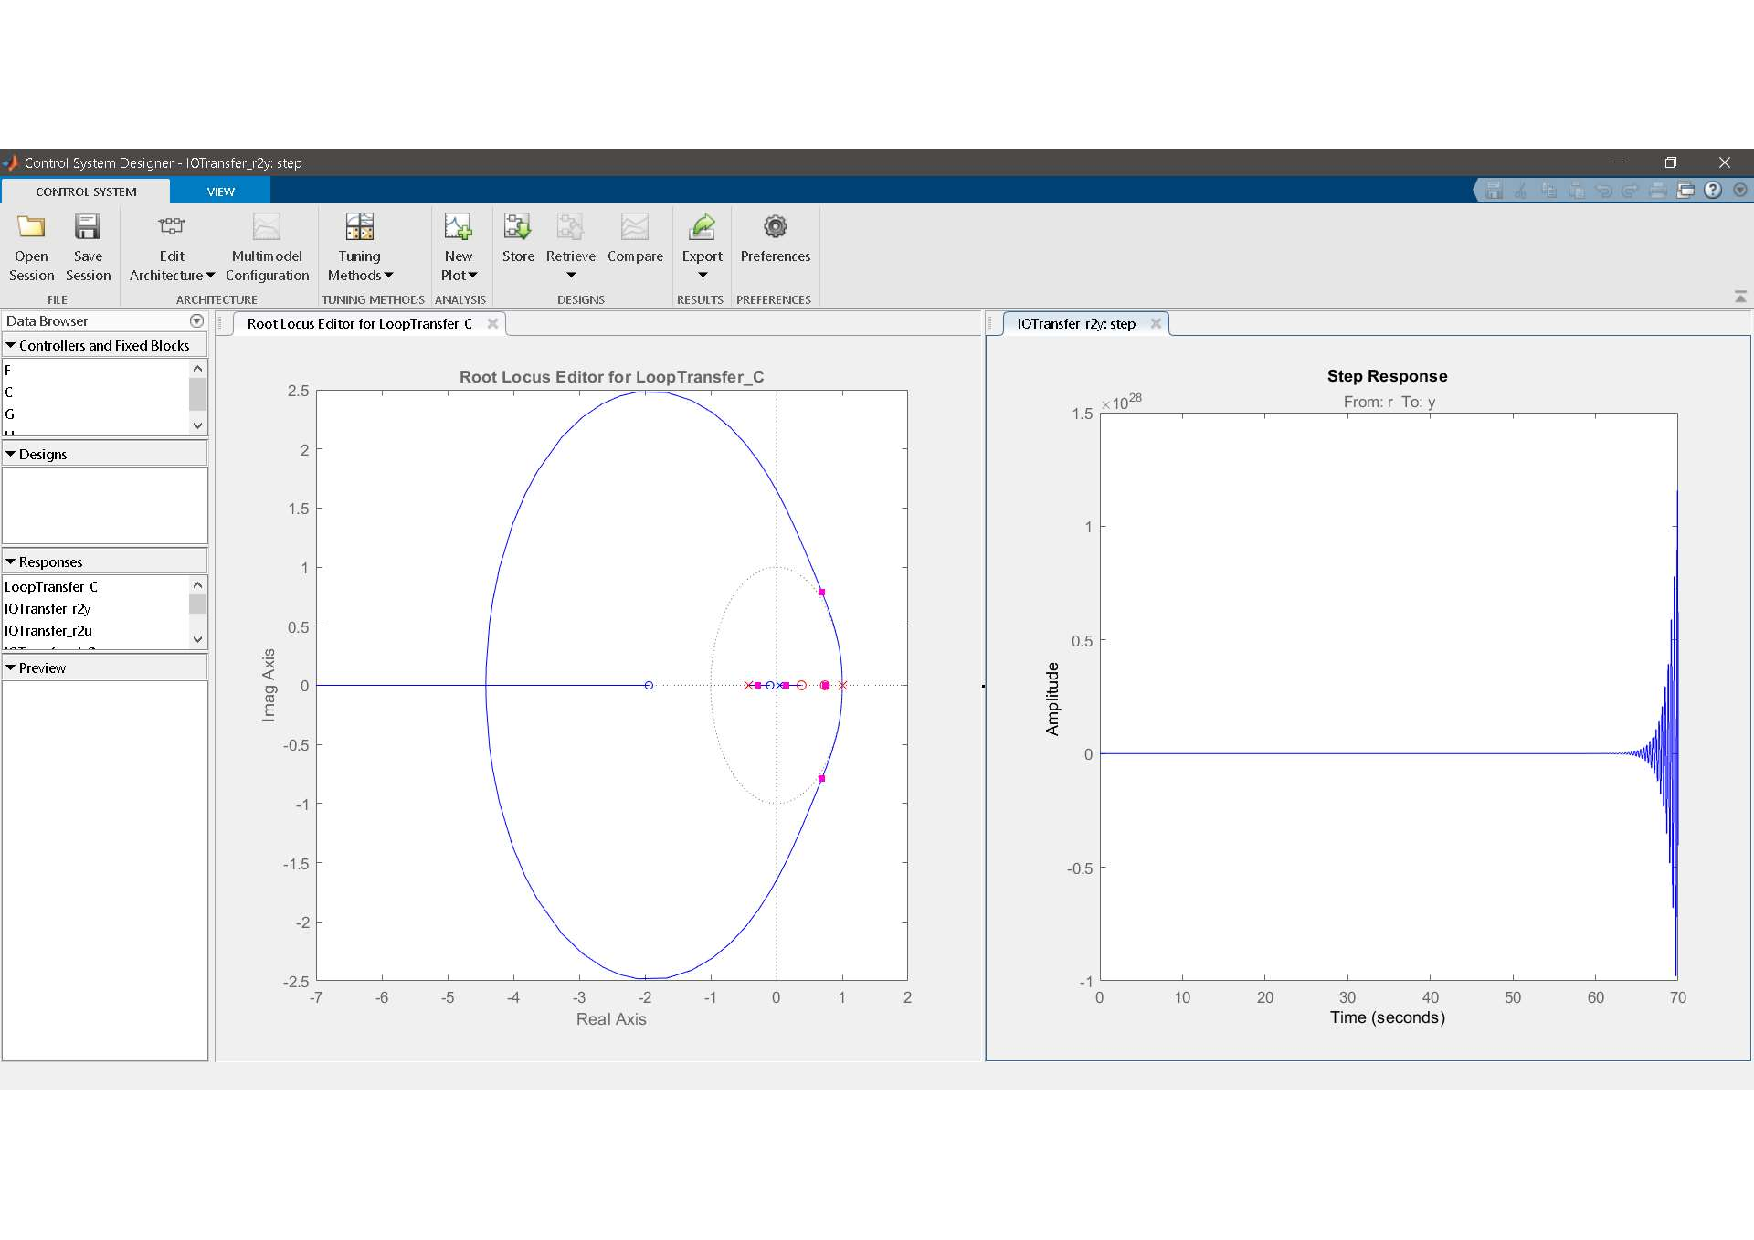
\includegraphics[clip, trim=0cm 3.5cm 0cm 2.8cm,scale=0.48]{images/figura 24.pdf}
  % izquierda,abajo,derecha,arriba
  \caption{Respuesta discretizada mediante el método Trapezoidal}
    \label{fig:figura 24}
\end{figure}
}
Mediante el método trapezoidal la discretización no es perfecta como
podemos observar, luego el método de discretización influye en la
respuesta lo que provoca que el sistema se vuelva inestable y que el
PID no cumpla su función.
  \end{tcolorbox}%
\newpage
\subsection{Actividad 14}
Diseñar un controlador analógico tipo PID (PD, PI, PID) para el
sistema servomotor de velocidad por el \textsc{método de Ziegler-Nichols} en
abierto y cerrado (si son posibles) y realizar su discretizacion con
$T=0.05$ aplicando el método trapezoidal y graficar la respuesta escalon
de posición unitario del sistema de control en bucle cerrado del
servomotor de velocidad a través de la herramienta \textsc{rltool}.

Para implementar el método Ziegler-Nichols en bucle abierto,
necesitamos que la respuesta ante entrada escalón sea la respuesta
aproximada de un sistema de primer orden con retardo y que cumpla
$0.15<d/tau<0.6$. Tras calcular los parámetros de nuestro sistema
obtenemos $d/tau = 3 > 0.6$ por lo que no es válido aplicar este
método. En caso de implementar el método de Ziegler-Nichols en bucle
cerrado, no se puede implementar debido a que nuestra planta es
estable independientemente del valor de la ganancia, imposibilitando
el calculo de los parámetros en el límite de la estabilidad, ya que
nunca se alcanza.

\begin{tcolorbox}[sharp corners, colframe=bluebox, title= Método de Ziegler-Nichols,breakable=unlimited]
$>>>$ [Kc,Pm,Wcg] = margin(Gvelocidad)\\
$>>>$ velocidadz = c2d(Gvelocidad,0.05,'zoh')\\
$>>>$ step(Gvelocidadz)\\
$>>>$ T1 = 0.2;\\
$>>>$ T2 = 0.1;\\
$>>>$ d = (3*(T1-T2))/2;\\
$>>>$ tau = T1-d;\\
$>>>$ d/tau\\

  \begin{tcolorbox}[sharp corners, colback = white]
    \color{gray}
\begin{verbatim}
Kc =
   Inf

Pm =
   Inf

Wcg =
   Inf

ans =
3.0000
\end{verbatim}
  \end{tcolorbox}%

 \end{tcolorbox}%



\newpage
\subsection{Actividad 15}
Diseñar un controlador analógico tipo PID (PD, PI, PID) para el
sistema servomotor de velocidad por el \textsc{método de Rivera-Morari} y de
síntesis directa y realizar su discretizacion con $T=0.05$ aplicando el
método de emparejaiento polos-ceros y graficar la respuesta escalón
unitaria del sistema de control en bucle cerrado del servomotor de
velocidad a través de la herramienta \textsc{rltool}.

\begin{tcolorbox}[sharp corners, colframe=bluebox, title= Controlador
  síntesis directa, breakable=unlimited]
Primero comprobamos si se puede controlar a través de este método. Para ello, 
el sistema debe ser estable en bucle abierto.

 $>>>$ step(Gvelocidad)
  \mkanscode{
\begin{figure}[H]
  \centering
  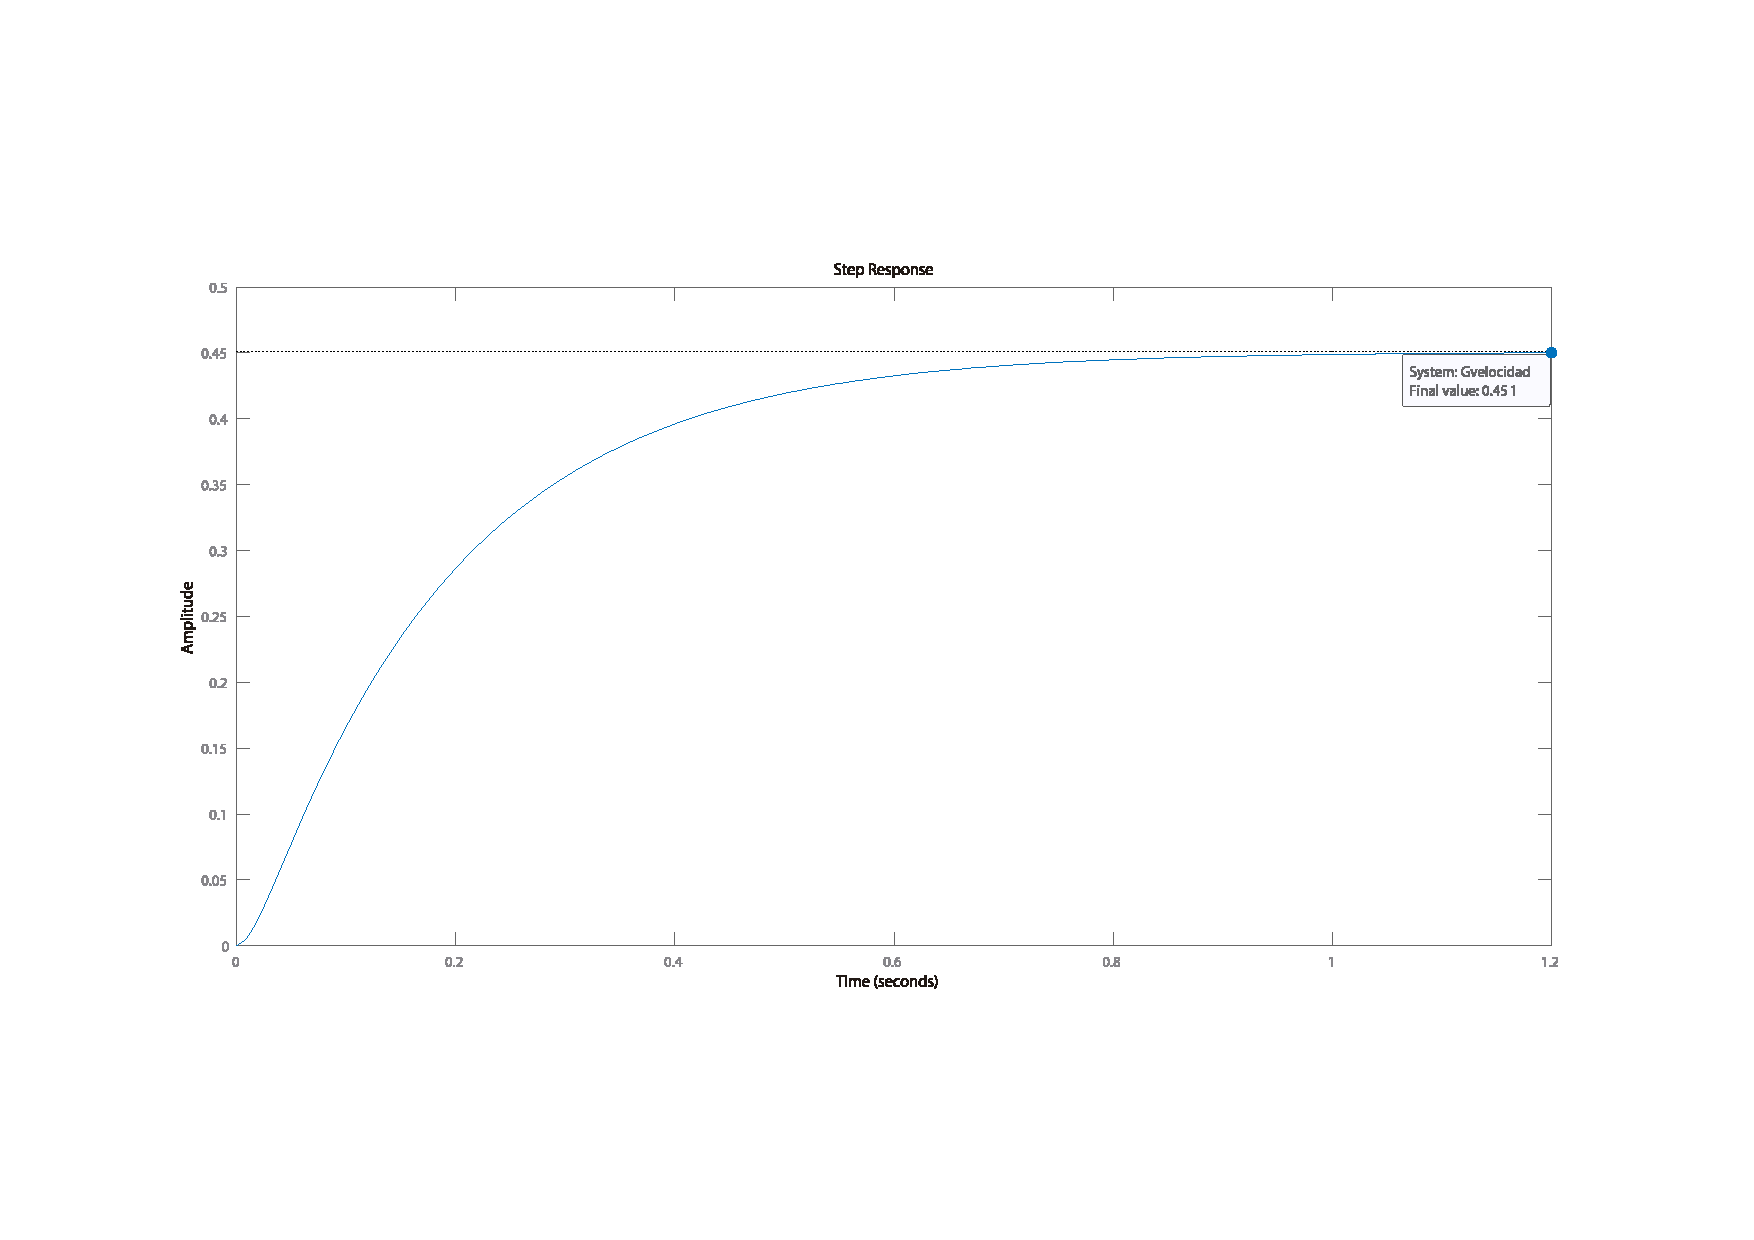
\includegraphics[clip, trim=4cm 4.5cm 3cm 4.5cm,scale=0.48]{images/figura 20.pdf}
  % izquierda,abajo,derecha,arriba
  \caption{Respuesta del sistema abierto frente a un escalón.}
    \label{fig:figura 20}
\end{figure}
  }
Según la respuesta del sistema en bucle abierto, es estable por lo que 
se puede aplicar. Nuestra planta es una planta de segundo orden
sobreamortiguada.

Calculamos los polos del sistema en bucle abierto

$>>>$ [polo1,polo2]= pole(Gvelocidad);

Se calculan los parámetros:\\
$k$ Es el valor final en bucle abierto, por lo tanto, $k = 0.451$.\\
$>>>$ tau\_1 =  1/63.5465\\
$>>>$ tau\_2 =  1/5.4951\\

Nuestra lamda debe ser mayor que $0.2*\tau_{max} = 0.2 *\tau_2 = 5.4951$.\\
Vamos a tomar\\
$>>>$ lambda = 6\\
$>>>$ k = 0.451;kp=(tau\_1+tau\_2)/(k*lamda);\\
$>>>$ ti = tau\_1 + tau\_2;\\
$>>>$ td = (tau\_1*tau\_2)/(tau\_1+tau\_2);\\
$>>>$ PID = pidstd(kp,ti,td)\\

  \vspace*{0.5em}
  \begin{tcolorbox}[sharp corners, colback = white]
    \color{gray}
\begin{verbatim}

PID =
 
             1      1          
  Kp * (1 + ---- * --- + Td * s)
             Ti     s          

  with Kp = 0.0731, Ti = 0.198, Td = 0.0145
 
Continuous-time PID controller in standard form
\end{verbatim}
  \end{tcolorbox}%
  \vspace*{0.5em}

$>>>$ C = c2d(PID,0.05,'matched')

    \vspace*{0.5em}
  \begin{tcolorbox}[sharp corners, colback = white]
    \color{gray}
\begin{verbatim}
C =
 
             1       Ts            z-1 
  Kp * (1 + ---- * ------ + Td * ------)
             Ti      z-1           Ts  

  with Kp = 0.0961, Ti = 0.26, Td = 0.0417, Ts = 0.05
 
Sample time: 0.05 seconds
Discrete-time PID controller in standard form
\end{verbatim}
  \end{tcolorbox}%
  $>>>$  step(kw*feedback(Gvelocidadz*C,kw))
      \vspace*{0.5em}
    \mkanscode{
\begin{figure}[H]
  \centering
  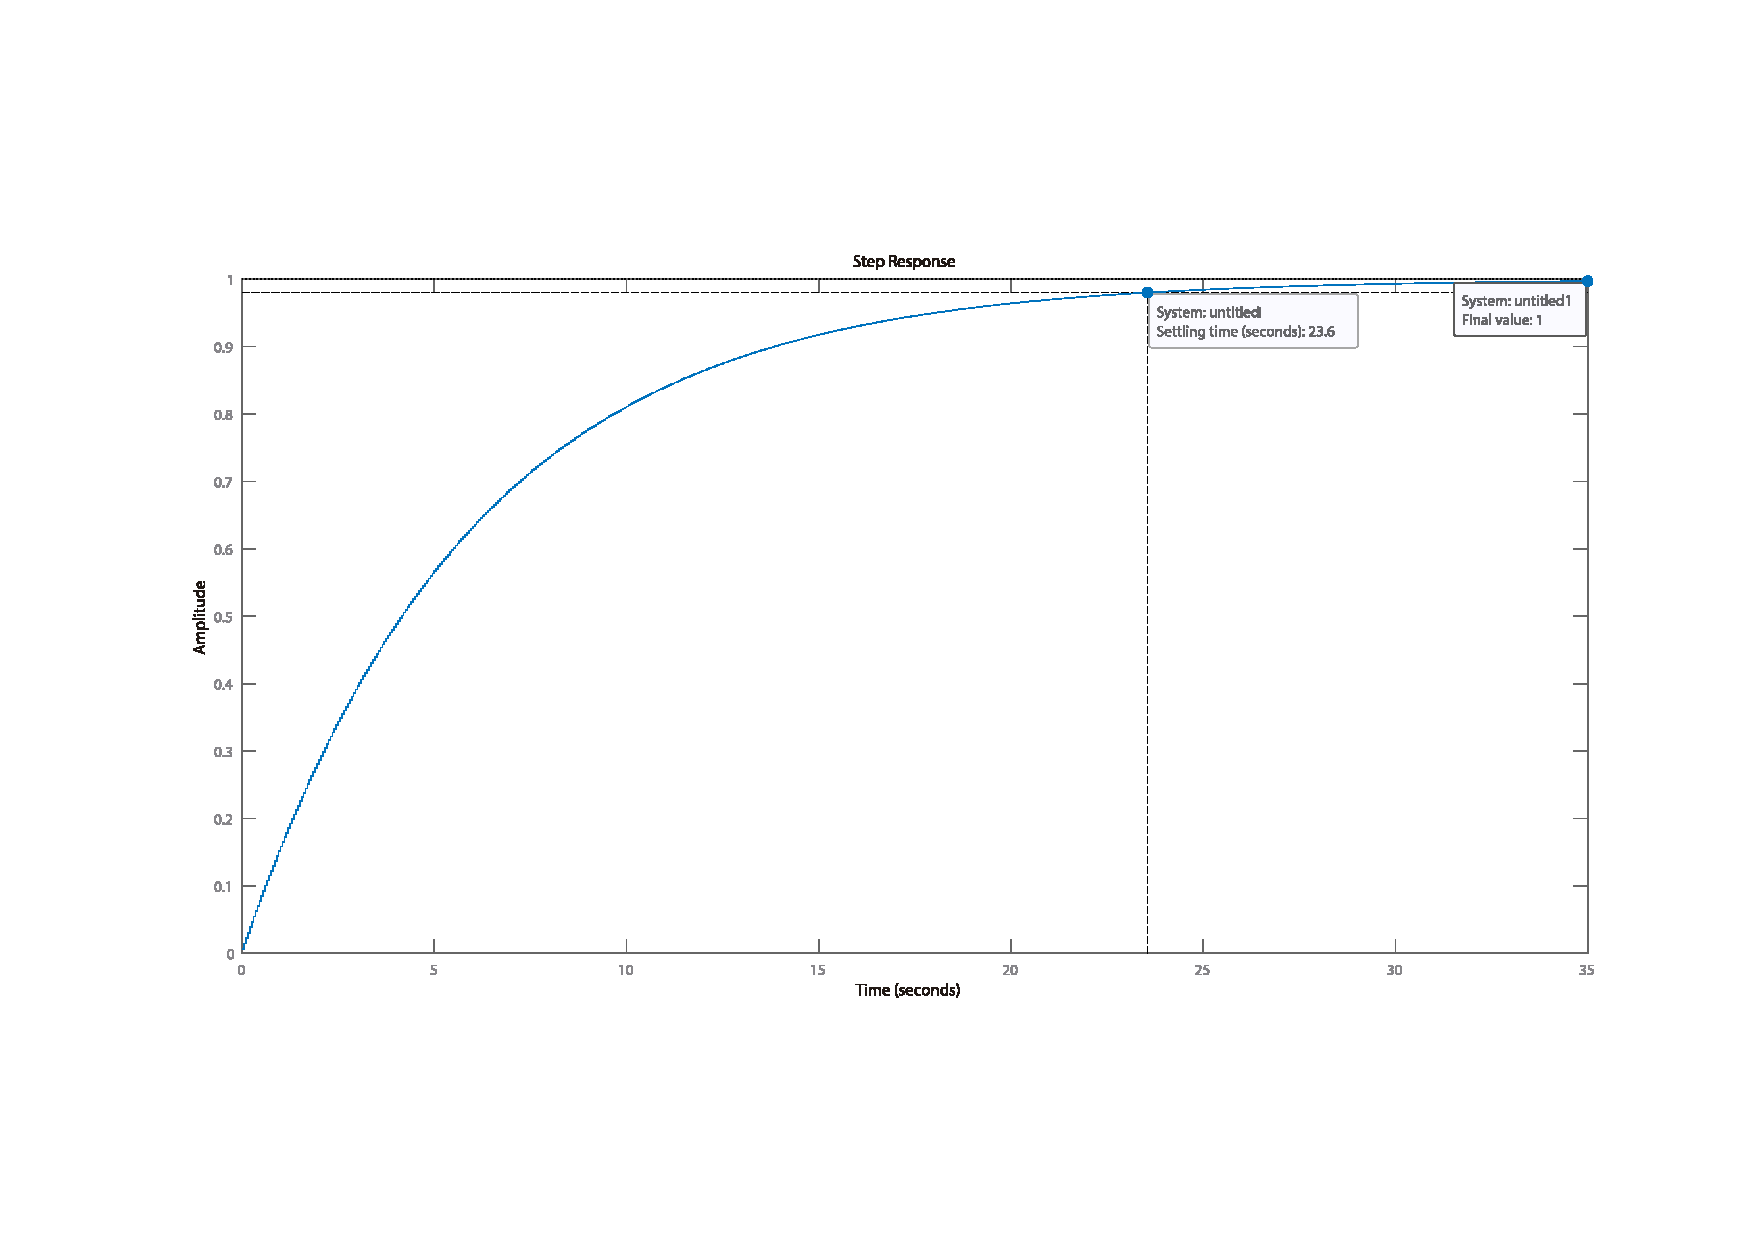
\includegraphics[clip, trim=2.5cm 3.5cm 2.8cm 4.5cm,scale=0.48]{images/figura 21.pdf}
  % izquierda,abajo,derecha,arriba
  \caption{Respuesta del sistema cerrado frente a un escalón.}
    \label{fig:figura 21}
\end{figure}
  }
\end{tcolorbox}%

\begin{tcolorbox}[sharp corners, colframe=bluebox, title= Controlador Rivera-Morari, breakable=unlimited]
Primero comprobamos si se puede controlar a través de este método. Para ello, 
el sistema debe ser estable en bucle abierto.

 $>>>$ step(Gvelocidad)
  \mkanscode{
\begin{figure}[H]
  \centering
  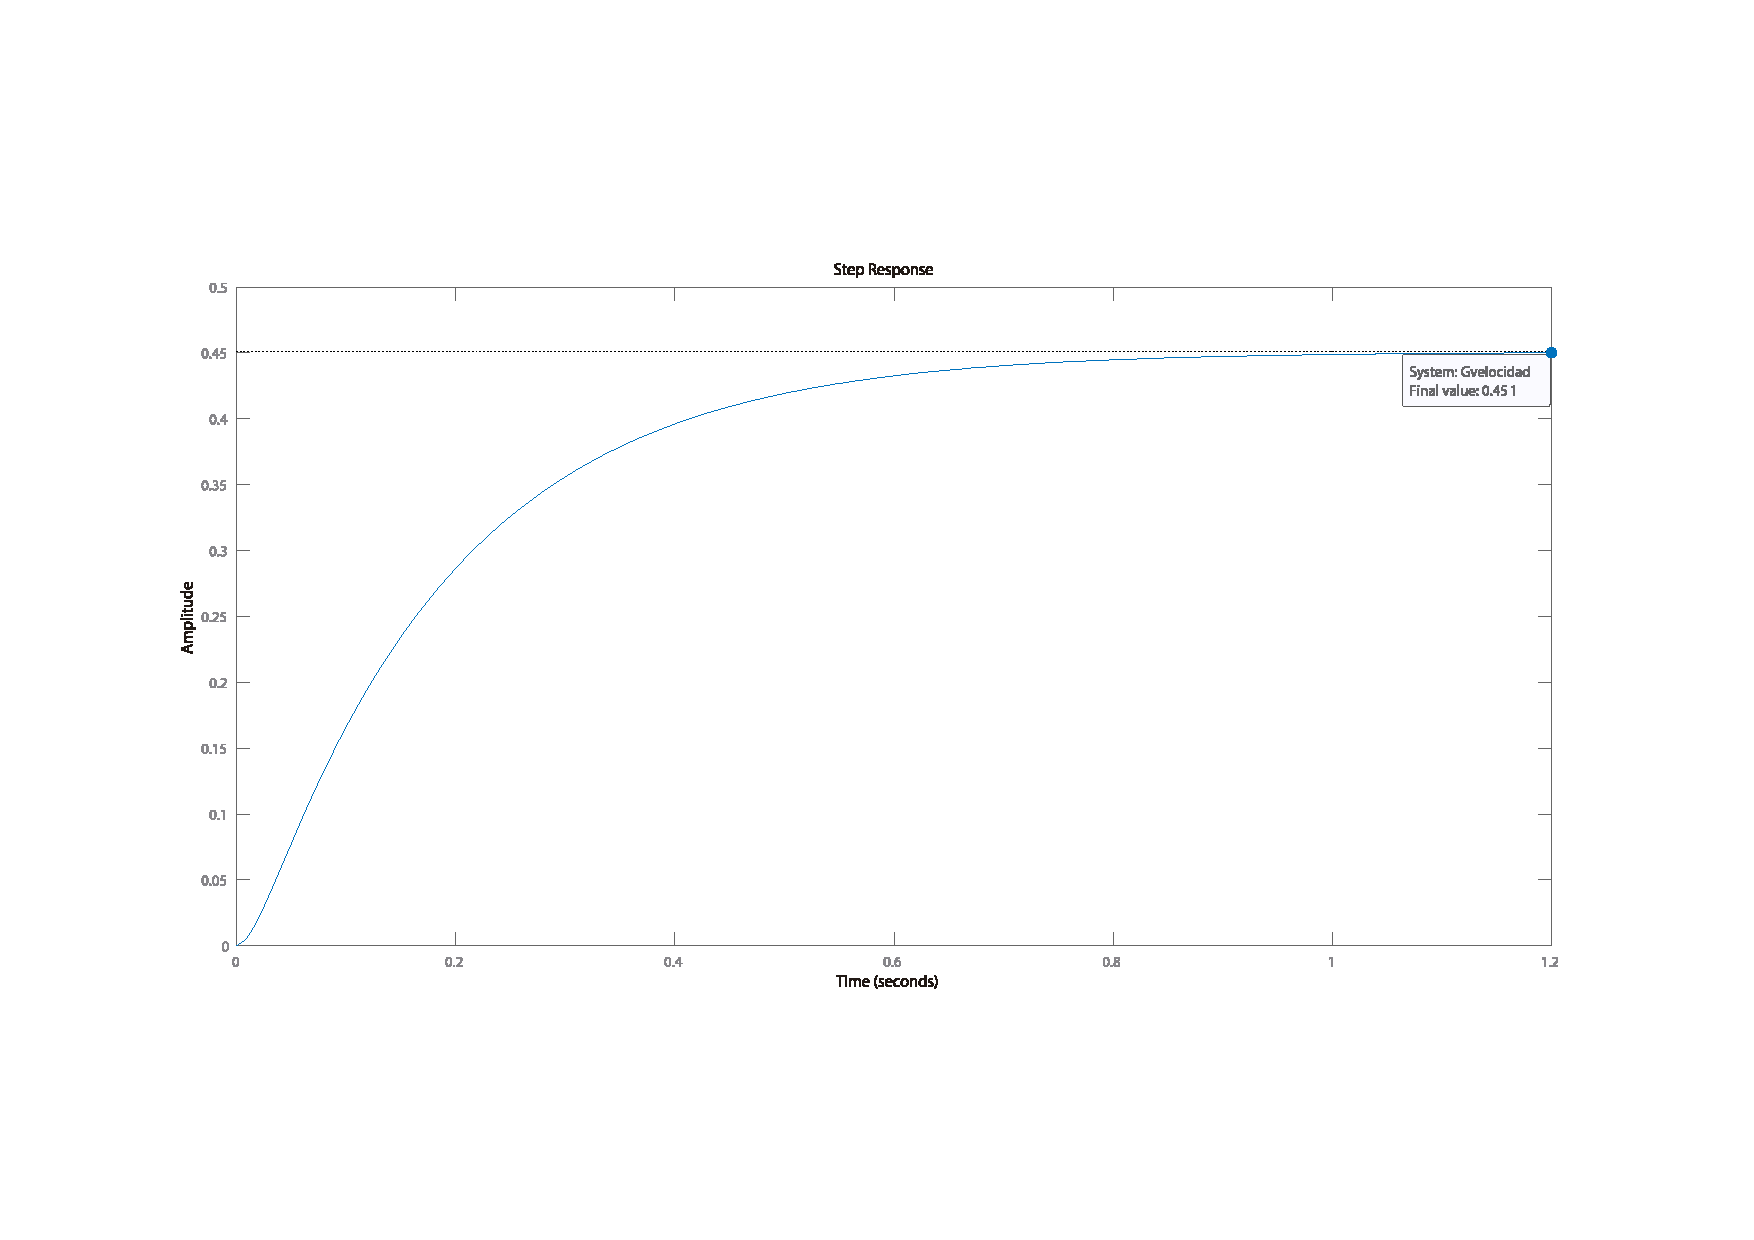
\includegraphics[clip, trim=4cm 4.5cm 3cm 4.5cm,scale=0.48]{images/figura 20.pdf}
  % izquierda,abajo,derecha,arriba
  \caption{Respuesta del sistema abierto frente a un escalón.}
    \label{fig:figura 20}
\end{figure}
}
A partir de la respuesta de nuestro sistema obtenemos:\\
$>>>$ k = 0.451\\
$>>>$ t632=0.119;t283=0.0773;\\

Obtenemos los parámetros para calcular nuestro PID:\\
$>>>$ d=3*(t632-t283)/2;tau=t632-d;\\
Es recomendable que $\lambda > 0.2*\tau=0.0113$\\
Y que cumpla que $\lambda/d > 1.7$, es decir, $\lambda > d*1.7 = 0.1063$\\
Elegiremos nuestro lamda\\
$>>>$ lamda = 1;\\
Llendo a la tabla de PI\\
$>>>$ kp = tau/(k*lamda);ti=tau;

Nuestro PI es:\\
$>>>$ PI = pidstd(kp,ti)
  \vspace*{0.5em}
  \begin{tcolorbox}[sharp corners, colback = white]
    \color{gray}
\begin{verbatim}
PI =
 
             1      1 
  Kp * (1 + ---- * ---)
             Ti     s 

  with Kp = 0.125, Ti = 0.0565
 
Continuous-time PI controller in standard form
\end{verbatim}
  \end{tcolorbox}%
  \vspace*{0.5em}

$>>>$ C = c2d(PID,0.05,'matched')

    \vspace*{0.5em}
  \begin{tcolorbox}[sharp corners, colback = white]
    \color{gray}
\begin{verbatim}
C =
 
             1       Ts  
  Kp * (1 + ---- * ------)
             Ti      z-1 

  with Kp = 0.189, Ti = 0.0851, Ts = 0.05
 
Sample time: 0.05 seconds
Discrete-time PI controller in standard form

\end{verbatim}
  \end{tcolorbox}%
  $>>>$  step(kw*feedback(Gvelocidadz*C,kw))
      \vspace*{0.5em}
    \mkanscode{
\begin{figure}[H]
  \centering
  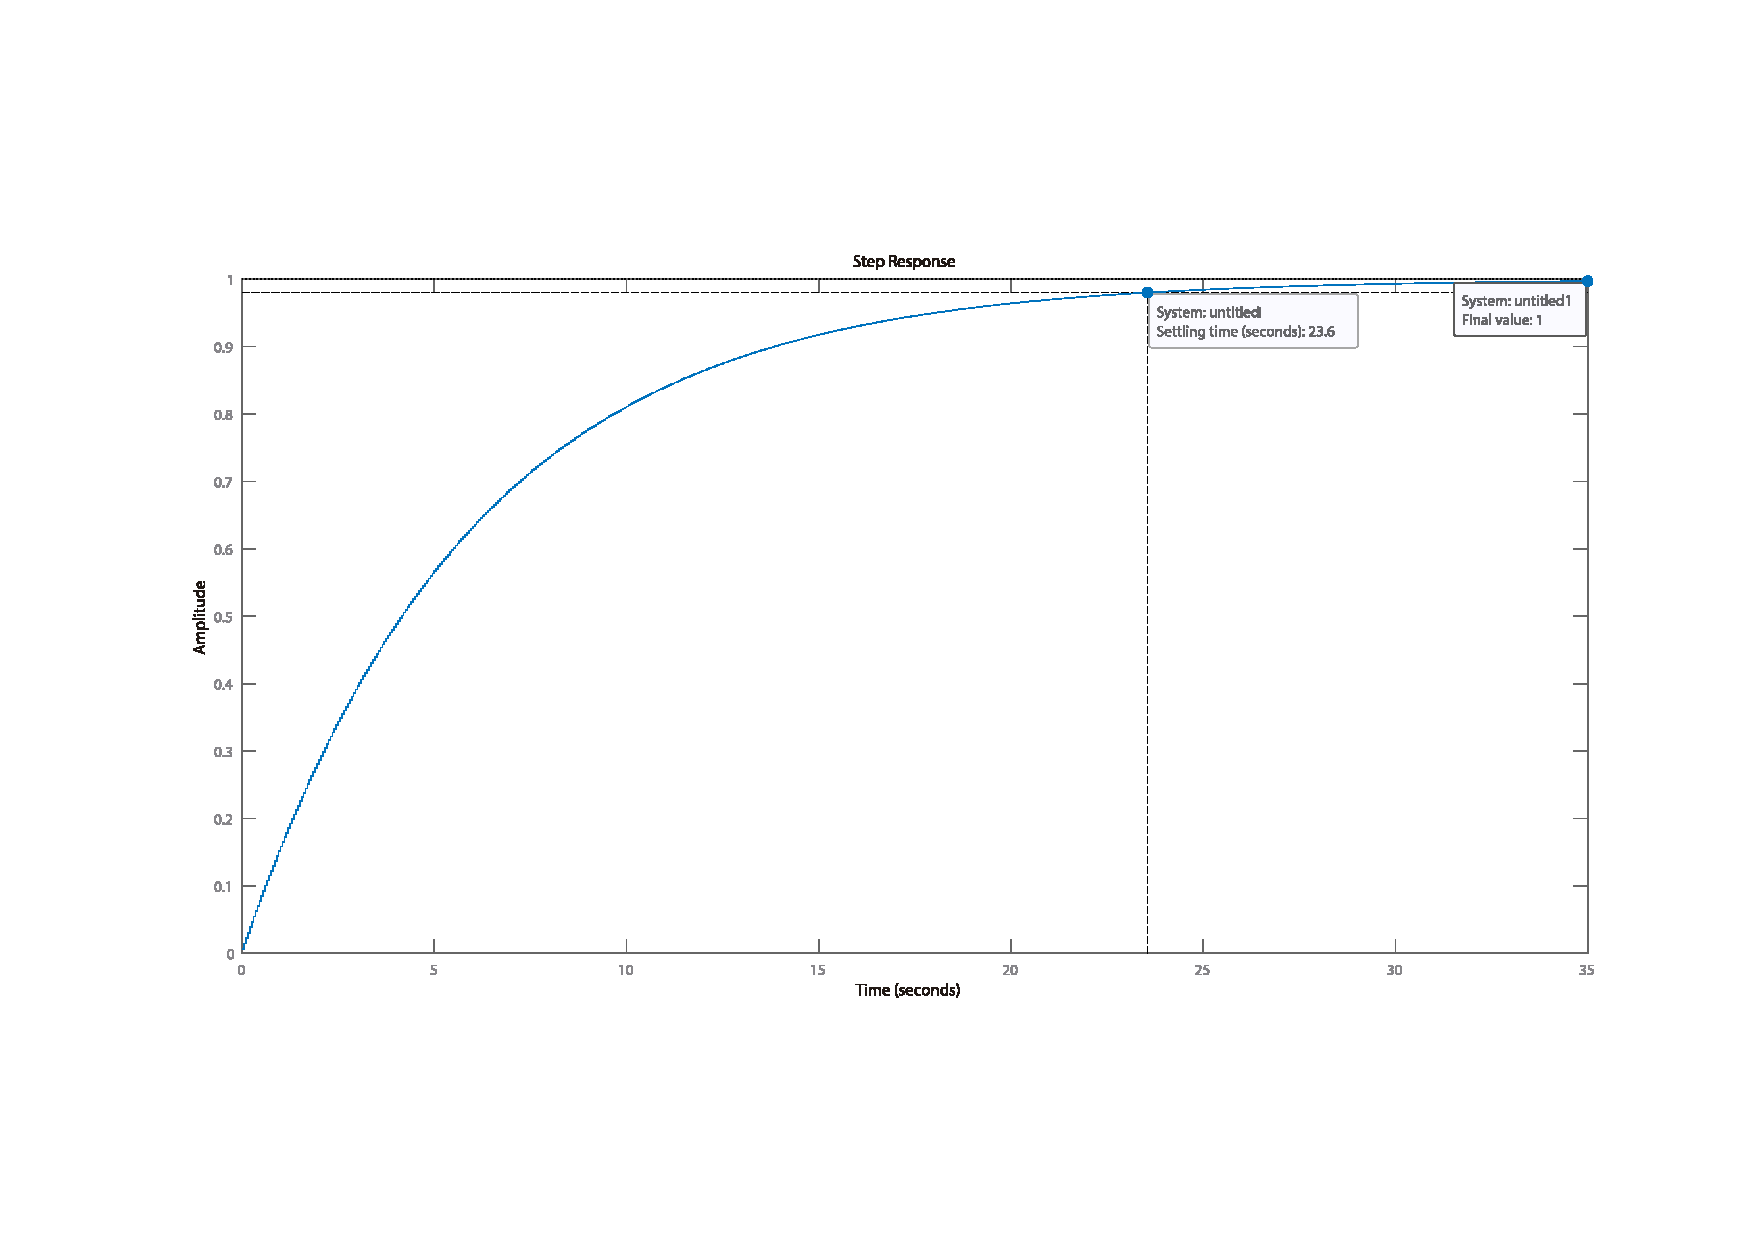
\includegraphics[clip, trim=2.5cm 3.5cm 2.5cm 4.5cm,scale=0.48]{images/figura 21.pdf}
  % izquierda,abajo,derecha,arriba
  \caption{Respuesta del sistema cerrado frente a un escalón.}
    \label{fig:figura 21}
\end{figure}
  }
  \end{tcolorbox}%
\newpage
\subsection{Actividad 16}
Diseñar un controlador vector de ganancias en espacio de estado
continuo para que el sistema en bucle cerrado en velocidad presente un
par de polos deseados con comportamiento críticamente amortiguado y
exhiba una frecuencia natural de $\omega_n$ de 10, asegurando error nulo ante
consigna velocidad con amplitud unitaria, partiendo de condiciones
iniciales nulas y especificando el resto de polos deseados a
suficiente distancia de los anteriores. Asumir que el estado es
observable. Posteriormente, graficar la respuesta del sistema de
control en velocidad en \textsc{MATLAB}.

Aunque \textsc{MATLAB} nos proporciona un modelo en el espacio de
estados para el sistema de velocidad hemos preferido hacerlo a mano
para seleccionar un vector de estado lógico (respecto a las variables
físicas que queremos controlar).

\begin{equation}
  \begin{split}
    \dfrac{V_s(s)}{V_e(s)} &= \dfrac{0.00544}{3.456\cdot10^{-5}s^2+0.002386s+0.01207}\\
    0.00544V_e(s) &= 3.456\cdot10^{-5}V_s(s)s^2+0.002386V_s(s)s+0.01207V_s(s)\\
    0.00544V_e(t) &=
    3.456\cdot10^{-5}V_s''(t)+0.002386V_s'(t)+0.01207V_s(t)\\
  \end{split}
\end{equation}
Seleccionamos como vectores de estado la velocidad y la
aceleración.
\begin{equation}
  \begin{split}
    x_1 &= V_s \ \ \ \ \ \ \ \ \dot x_1 = V_s' = x_2\\
    x_2 &= V_s' \ \ \ \ \ \ \ \ \dot x_2 = V_s''
    \end{split}
  \end{equation}
\begin{equation}
  \begin{split}
0.00544 u &=  3.456 \cdot 10^{-5} \dot x_2 + 0.002386 x_2 + 0.01207 x_1\\
\dot x_2 &= 157.4074 u - 69.0394x_2-349.2477x_1\\
\end{split}
\end{equation}

\begin{equation}
  \begin{bmatrix}
    \dot x_1 \\
    \dot x_2
\end{bmatrix} =
\begin{bmatrix}
  0 & 1\\
  -349.2477 & -69.0394
\end{bmatrix}
\begin{bmatrix}
  x_1\\
  x_2
\end{bmatrix}
+
\begin{bmatrix}
  0\\
  157.4074
\end{bmatrix}
\begin{bmatrix}
  u
\end{bmatrix}
\end{equation}

\begin{equation}
  y = 
  \begin{bmatrix}
1 & 0
\end{bmatrix}
\begin{bmatrix}
  x_1\\
  x_2
\end{bmatrix} 
\end{equation}

\newpage
\lstinputlisting[language=MATLAB]{./codes/actividad16.m}
\begin{tcolorbox}[sharp corners, colframe=bluebox, title= Respuesta
  del sistema en tiempo continuo]
 % $>>>$ ltiview(\textcolor{blue}{`lsim'},kr*feedback(PDI\_10*Gposicionz,kr))
  \vspace*{0.35em}
  \mkanscode{
\begin{figure}[H]
  \centering
  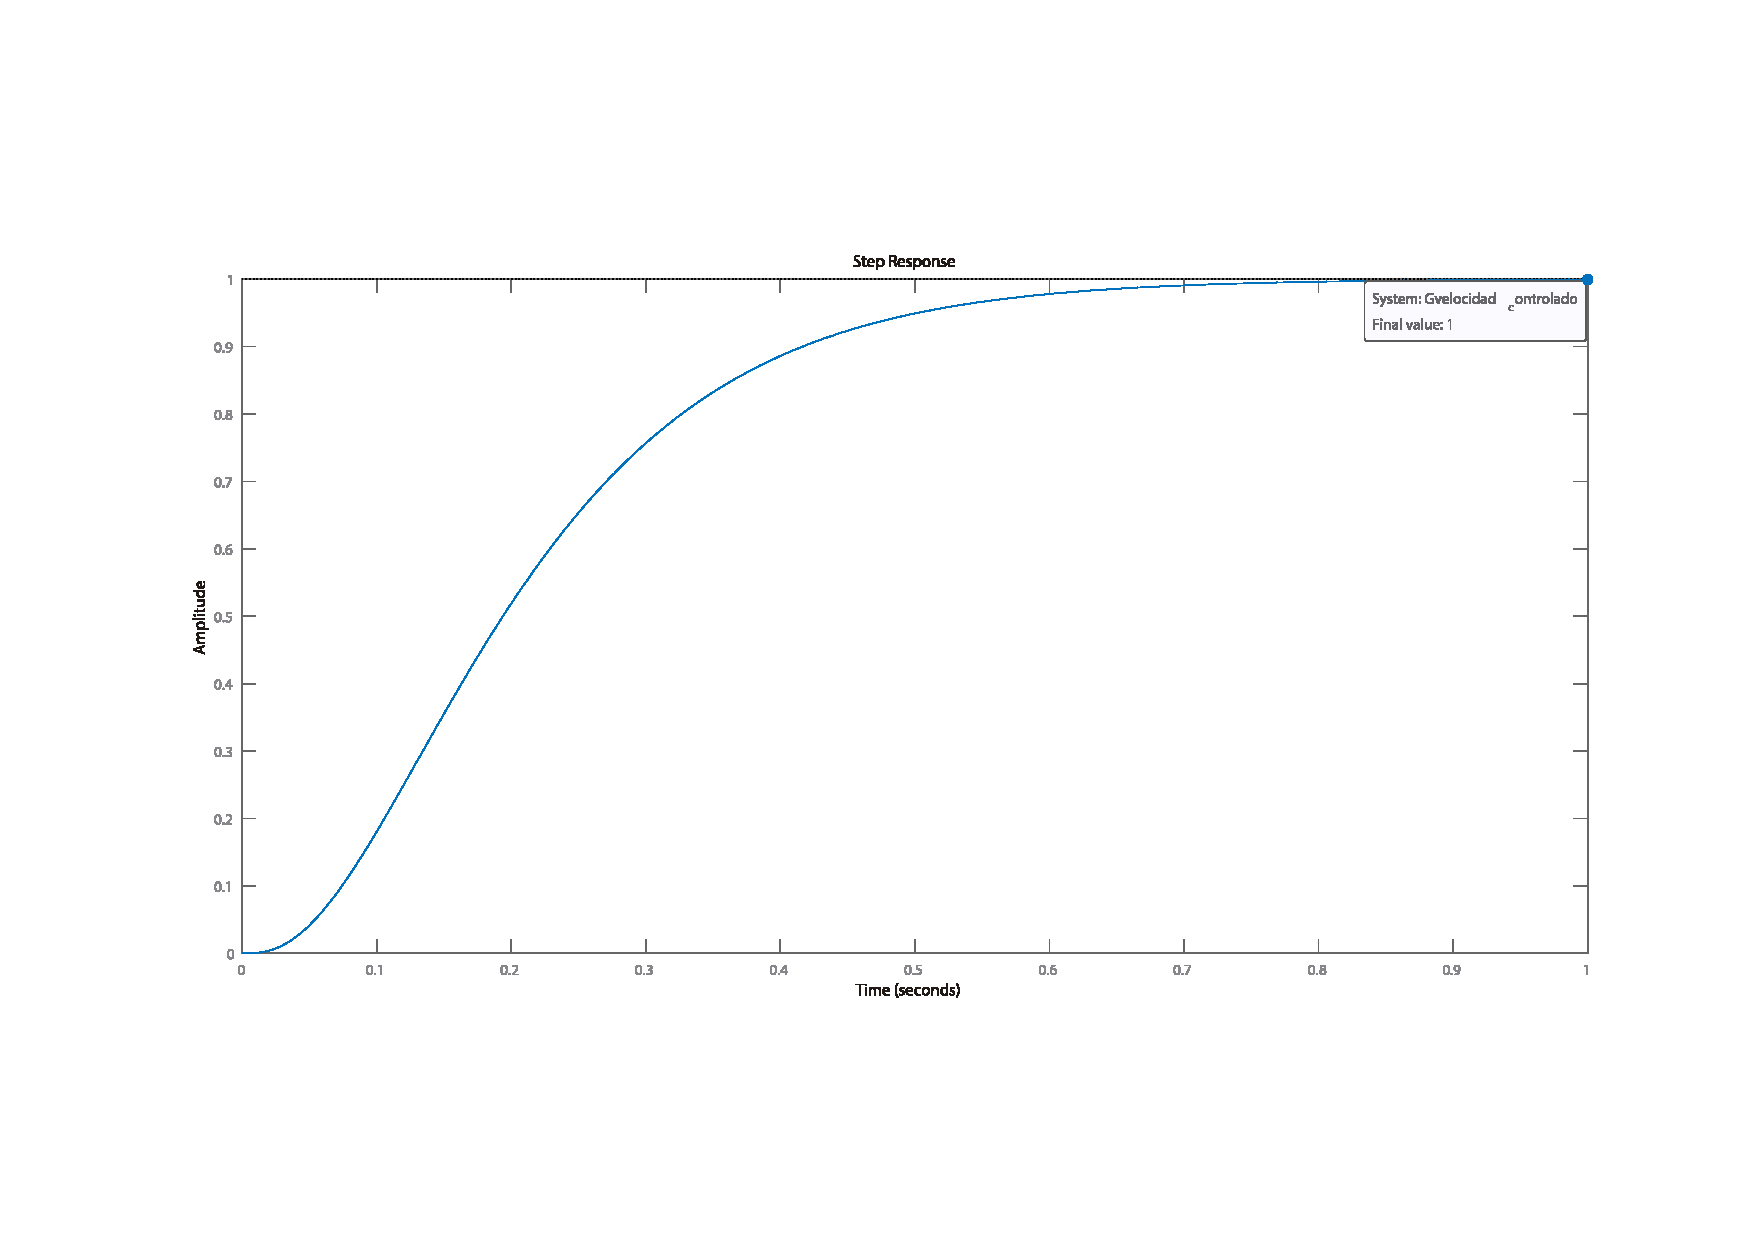
\includegraphics[clip, trim=2.5cm 4.5cm 2.5cm 4.25cm,
  scale=0.5]{images/figura 18.pdf}
  % izquierda,abajo,derecha,arriba
  \caption{Respuesta del sistema con error nulo.}
    \label{fig:figura 18}
\end{figure}
}
\vspace*{0.35em}
  \end{tcolorbox}%
\newpage
\subsection{Actividad 17}
Repetir el diseño en formato digital asumiendo un $T=0.05$,
partiendo de la función de transferencia discretizada del sistema y
polos deseados obtenidos a partir de la relación $z=e^{sT}$.

\lstinputlisting[language=MATLAB]{./codes/actividad17.m}

\begin{tcolorbox}[sharp corners, colframe=bluebox, title= Respuesta
  del sistema en tiempo discreto]
 % $>>>$ ltiview(\textcolor{blue}{`lsim'},kr*feedback(PDI\_10*Gposicionz,kr))
  \vspace*{0.35em}
  \mkanscode{
\begin{figure}[H]
  \centering
  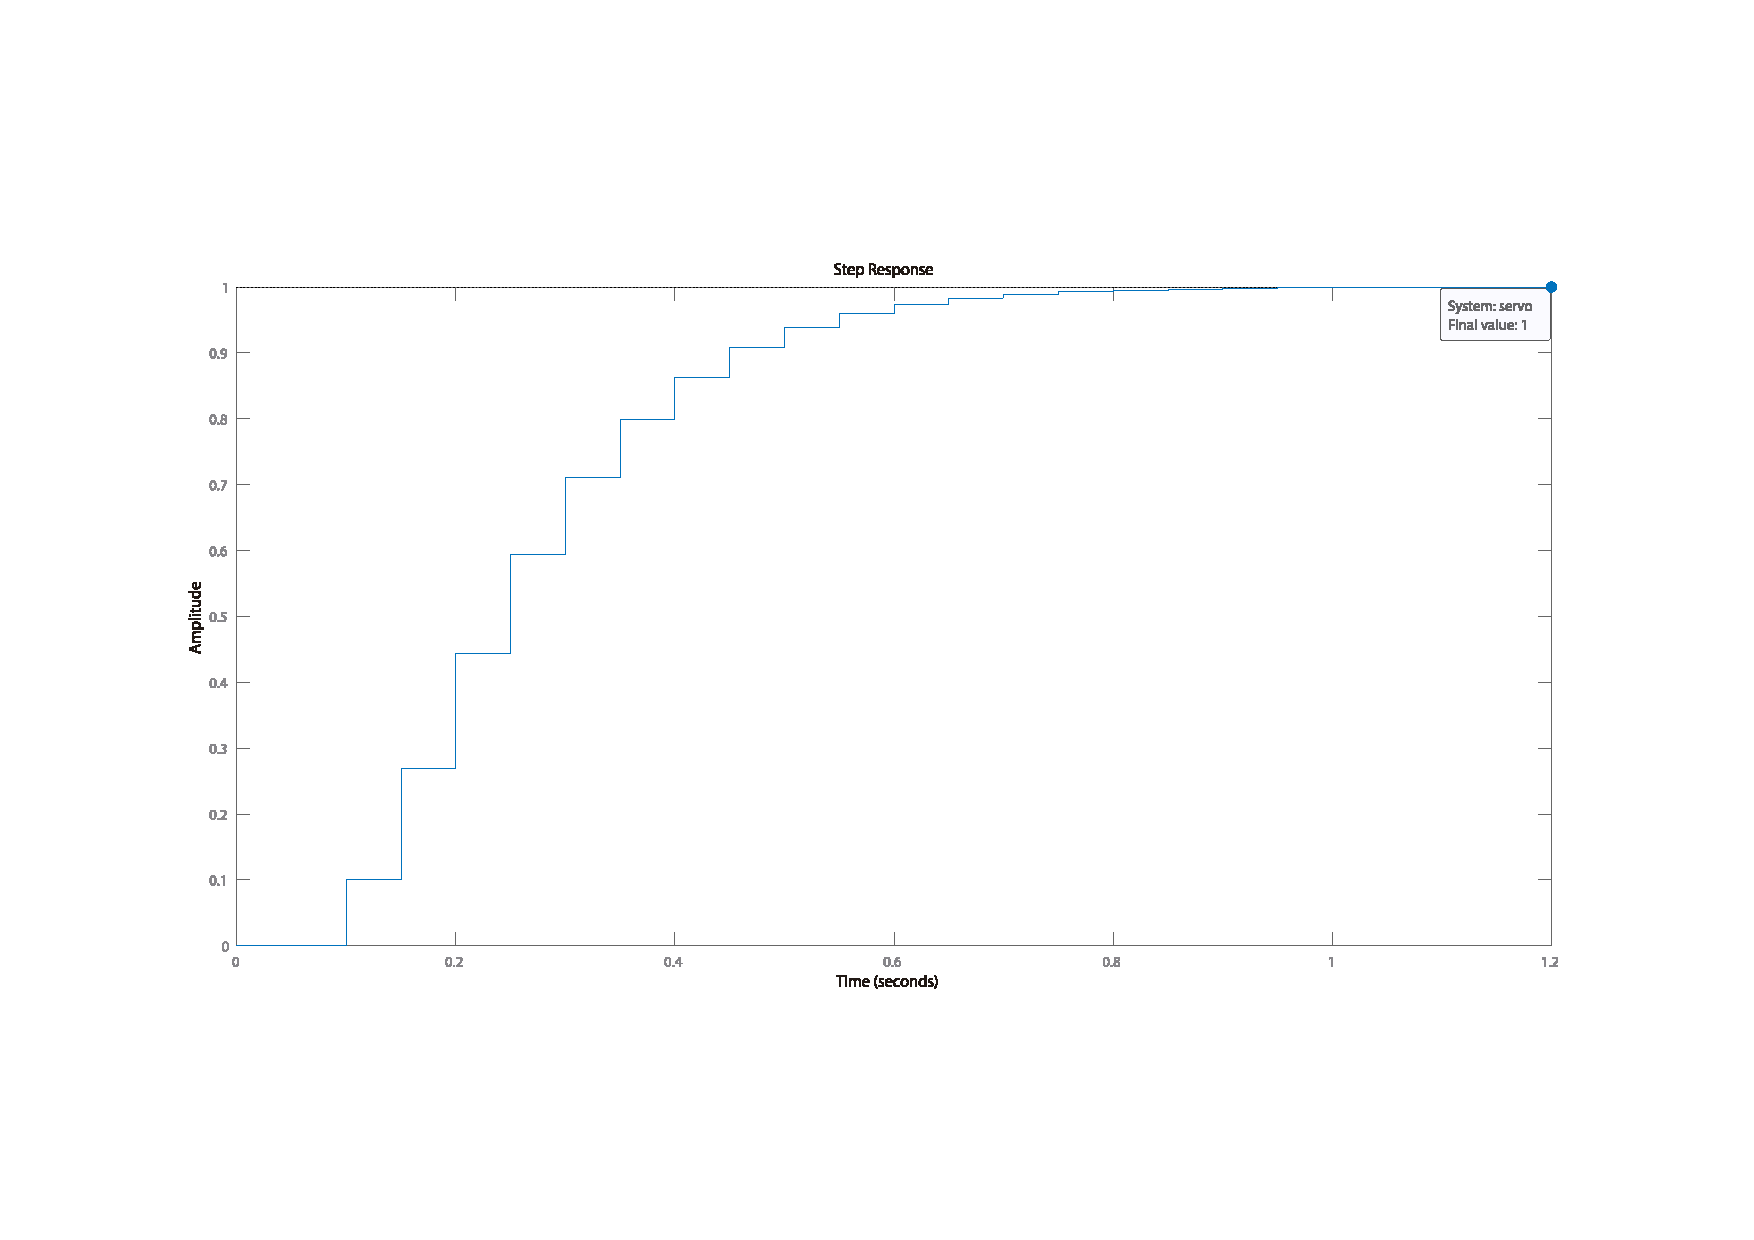
\includegraphics[clip, trim=2.5cm 4.5cm 2.5cm 4.25cm,
  scale=0.5]{images/figura 19.pdf}
  % izquierda,abajo,derecha,arriba
  \caption{Respuesta del sistema con error nulo.}
    \label{fig:figura 18}
\end{figure}
}
\vspace*{0.35em}
  \end{tcolorbox}%
\newpage
\section{Código \tiny{escrito en \textbf{MATLAB}}}
\UseRawInputEncoding
\lstinputlisting[language=MATLAB]{./codes/trabajo_cpc.m}

